\documentclass[12pt,a4paper,twoside]{report}
\usepackage{graphicx} % Required for inserting images
\usepackage[utf8]{inputenc}
\usepackage{natbib}
%\usepackage[english]{babel}
\usepackage[portuges]{babel} %
\usepackage[margin=2.5cm]{geometry}
%\usepackage[toc,page]{appendix}
\usepackage{fancyhdr}
\usepackage{graphicx} 
\usepackage{float}
\usepackage{wrapfig}
\usepackage{indentfirst}
\usepackage{multirow}
\usepackage{amsmath}
\usepackage{wrapfig}
\usepackage{placeins}
\usepackage{subcaption} 
\usepackage{booktabs}
\usepackage{tabularx}
\usepackage{pdfpages}
\usepackage{parskip}
\usepackage{url}
\usepackage[acronym]{glossaries}
\usepackage{afterpage}
\usepackage{booktabs,tabularx}
\usepackage{lscape}
\renewcommand{\tabularxcolumn}{m}
\makeglossaries


\usepackage{fancyhdr,lipsum}

\usepackage{listings}
\renewcommand{\lstlistingname}{Listagem}
%\renewcommand*{\lstlistlistingname}{Lista de Listagens}
\lstset{
 xleftmargin = 1cm,
 basicstyle=\footnotesize, 
 numbers=left, 
 captionpos=b,
 columns=fullflexible,
 breaklines=true,
 frame=single
}

\begin{document}
%%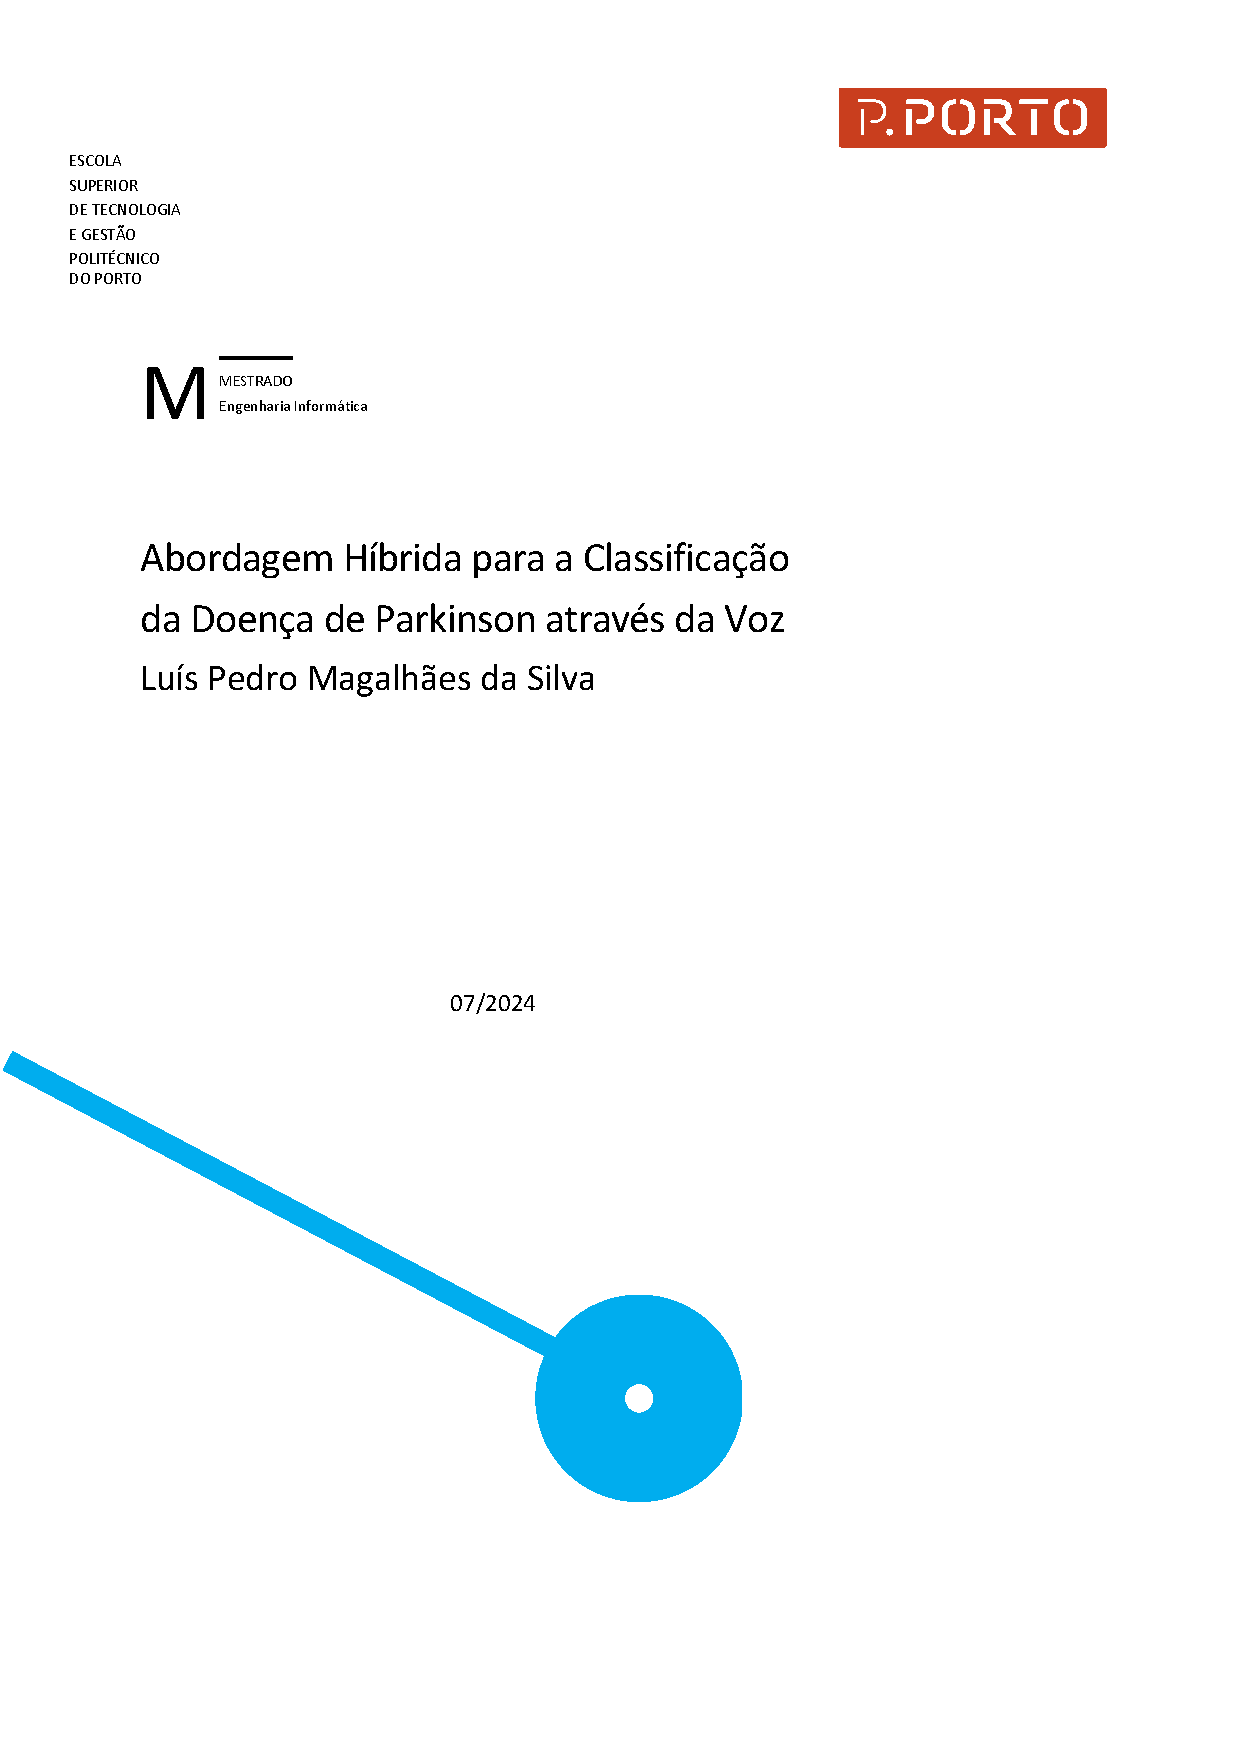
\includepdf[landscape=true,pages=1]{capas/ESTG-CAPA Mestrado-Final Version English_2 capa.pdf}
%%<\includepdf[landscape=true,pages=2]{capas/ESTG-CAPA Mestrado-Final Version English_2 capa.pdf}
\pagenumbering{roman}
%%%% colocar aqui acrónimos
\newacronym{AUC}{AUC}{Valor da área sob a curva ROC}
\newacronym{AdaBoost}{AdaBoost}{\textit{Adaptative Boosting}}
\newacronym{ANOVA}{ANOVA}{\textit{Analysis of Variance}}
\newacronym{BT}{BT}{\textit{Bagged Tree}}
\newacronym{CRISP-DM}{CRISP-DM}{\textit{Cross Industry Standard Process
for Data Mining}}
\newacronym{DBS}{DBS}{\textit{Deep Brain Stimulation}}
\newacronym{DP}{DP}{Doença de \textit{Parkinson}}
\newacronym{DT}{DT}{\textit{Decision Tree}}
\newacronym{ECFS}{ECFS}{\textit{Eigenvector Centrality Feature Selection}}
\newacronym{EMG}{EMG}{Eletromiografia}
\newacronym{estg}{ESTG}{Escola Superior de Tecnlogia e Gestão}
\newacronym{FN}{FN}{Falso Negativo}
\newacronym{FP}{FP}{Falso Positivo}
\newacronym{GB}{GB}{\textit{Gradient Boosting}}
\newacronym{GUI}{GUI}{\textit{Graphical User Interface}}
\newacronym{IA}{IA}{Inteligência Artificial}
\newacronym{LD}{LD}{\textit{Linear Descriminant}}
\newacronym{L-Dopa}{L-Dopa}{\textit{Levodopa}}
\newacronym{LR}{LR}{\textit{Logistic Regression}}
\newacronym{LOSO}{LOSO}{\textit{Leave one subject out}}
\newacronym{MAE}{MAE}{\textit{Mean Average Error}}
\newacronym{MAMa}{MAMa}{\textit{Minimum Average maximum Tree}}
\newacronym{ML}{ML}{\textit{Machine Learning}}
\newacronym{MLP}{MLP}{\textit{Multilayer Perceptron}}
\newacronym{MRI}{MRI}{\textit{Magnetic resonance imaging}}
\newacronym{mRMR}{mRMR}{\textit{Minimum Redundancy-maximum relevance}}
\newacronym{MSE}{MSE}{\textit{Mean Squared Error}}
\newacronym{NB}{NB}{\textit{Naive Bayes}}
\newacronym{NN}{NN}{\textit{K-Nearest Neighbors}}
\newacronym{PCA}{PCA}{\textit{Principal Component Analysis}}
\newacronym{RBF}{RBF}{\textit{Radial Based Function}}
\newacronym{RF}{RF}{\textit{Random Forest}}
\newacronym{RFE}{RFE}{\textit{Recursive Feature Elimination}}
\newacronym{RL}{RL}{\textit{Reinforcement Learning}}
\newacronym{RMSE}{RMSE}{\textit{Root Mean Squared Error}}
\newacronym{ROC}{ROC}{\textit{Receiver Operating Characteristics}}
\newacronym{SL}{SL}{\textit{Supervised Learning}}
\newacronym{SMOTE}{SMOTE}{\textit{Synthetic Minority Oversampling Technique}}
\newacronym{SVD}{SVD}{\textit{Singular Value Decomposition}}
\newacronym{SVM}{SVM}{\textit{Support Vector Machine}}
\newacronym{TAC}{TAC}{Tomografia Computorizada}
\newacronym{TQWT}{TQWT}{\textit{Tunable wavelet transform approach}}
\newacronym{UL}{UL}{\textit{Unsupervised Learning}}
\newacronym{VIF}{VIF}{Variância Inflacionária de Fator}
\newacronym{VN}{VN}{Verdadeiro Negativo}
\newacronym{VP}{VP}{Verdadeiro Positivo}
\newacronym{XGBoost}{XGBoost}{\textit{Extreme Gradient Boost}}



\chapter*{Declaração de Integridade}

Eu, Luís Pedro Magalhães da Silva, estudante nº 8220025, do Mestrado de Engenharia Informática, da Escola Superior de Tecnologia e Gestão do Instituto Politécnico do Porto, declaro que não fiz plágio nem auto-plágio, pelo que o trabalho intitulado “Abordagem Híbrida para a Classificação da Doença de Parkinson através da voz” é original e da minha autoria, não tendo sido usado previamente para qualquer outro fim. Mais declaro que todas as fontes usadas estão citadas, no texto e na bibliografia final, segundo as regras de referenciação adotadas na instituição.

\chapter*{Agradecimentos}
%Opcional, capítulo pode ser comentado
Como nota da felicidade por mim expressa, quero deixar umas notas de agradecimento às diversas pessoas que me ajudaram ao longo de todo o meu percurso académico, nomeadamente Professores e Colegas.

Primeiramente, quero agradecer de forma mais específica, ao Professor Doutor João Ricardo Martins Ramos pela sua inestimável assistência no fornecimento de \textit{insights}, nomeadamente na escolha do tema, bem como em conselhos durante a fase de revisão literatura, bem como no fornecimento de \textit{feedback} durante o desenvolvimento, bem como na descrição dos passos a realizar.

De seguida, gostaria também de deixar um agradecimento especial aos meus colegas de Mestrado e amigos com os quais tive a oportunidade de partilhar experiências realizadas nesta dissertação, bem como através dos quais foi possível obter bastante conhecimento.

Por fim, gostaria de expressar a minha mais profunda gratidão a todos aqueles que me ajudaram a manter-me motivado e inspirado durante esta dissertação, sendo que nem sempre é um processo fácil, sendo exaustivo e desafiante.

Esta dissertação é dedicada aos Familiares mais próximos, dos quais destaco os meus pais e irmão, cujo apoio, incentivo e
o amor será para sempre minha força, resiliência e abrigo para tudo o que conquisto e poderei conquistar na vida.

\chapter*{Resumo}

A \gls{DP} é  a segunda doença Neurodegenerativa mais presente, apenas superada pela Doença de \textit{Alzheimer}, e atualmente estima-se que apresente uma incidência entre as 7 a 10 milhões de pessoas, sendo presentes em pessoas com uma idade mais avançada (raramente acontece antes dos 50 anos). 

À medida que a população mundial envelhece,  a sua prevalência aumenta de forma diretamente proporcional. Sabe-se que não existe nenhuma forma efetiva de realizar o diagnóstico da doença de \textit{Parkinson}, sendo que o presente estudo representa a possibilidade de ser feito um diagnóstico prévio, através de algoritmos de \gls{ML}  baseados num conjunto de dados da voz. 

Como o Conjunto de dados adquirido é desbalanceado e apresenta um problema de elevada dimensão (conjunto de features bastante numeroso), estudou-se o conjunto de dados em 3 vertentes distintas: \textit{Dataset} Completo, \textit{Dataset} dividido por género e \textit{Dataset} dividido por conjunto de \textit{features}.

Nas 3 divisões do conjunto de dados, estudaram-se diversos algoritmos de forma individual e também se utilizou um Ensemble, com a utilização dos diversos classificadores, de forma a tornar o modelo mais robusto. 

Nos resultados, obteve-se os melhores resultados, no estudo com o \textit{Dataset} completo, em que se promoveu um Sistema Híbrido de Classificação com a utilização de \gls{SMOTE}, algoritmos de Seleção de features para a redução da dimensionalidade e métodos \textit{Ensemble}.

Os resultados indicam que a utilização de técnicas de \gls{ML}  baseadas num conjunto de dados da voz, pode ser uma boa possibilidade para a deteção prévia da \gls{DP}, permitindo desta forma, um tratamento mais especializado e eficaz para o paciente.


\textbf{Palavras-chaves:} \textit{Parkinson}, \textit{Machine Learning}, \textit{SMOTE}, \textit{Feature Selection}, \textit{ENSEMBLE}, \textit{Classification}.


\chapter*{\textit{Abstract}}

\textit{Parkinson's Disease (PD) is the second most common neurodegenerative disease,
second only to Alzheimer's and is estimated to have an incidence of between
7 to 10 million people, and is present in people at a more advanced age
(it rarely occurs before the age of 50).
As the world's population ages, its prevalence increases di- proportionally.
proportionally. It is known that there is no effective way of making the
diagnosis of Parkinson's disease, so this study represents the ability to diagnose Parkinson's disease.
perform a preliminary diagnosis using Machine Learning algorithms based on a set of voice data.
As the acquired data set is unbalanced and presents a high-dimensional problem, it has to be analyzed.
problem, we propose the study of various algorithms with different pre-processing stages.
data processing, namely the proposal for a Hybrid Classification System.
with the use of SMOTE, feature selection algorithms to reduce dimensionality and Ensemble methods.}

\textbf{\textit{Keywords}:} \textit{Parkinson}, \textit{Machine Learning}, \textit{SMOTE}, \textit{Feature Selection}, \textit{ENSEMBLE}, \textit{Classification



\cleardoublepage

\tableofcontents % Gera índice

\listoffigures % Gera índice de figuras

\listoftables % Gera índice de tabelas



%\lstlistoflistings % Gera índice de listagens

\printglossary[type=\acronymtype,title=Acrónimos] % Gera índice de acrónimos

\pagenumbering{arabic}

\chapter{Introdução}

O Primeiro Capítulo apresenta um breve enquadramento do tema em estudo, ou seja, uma contextualização e posterior enquadramento, onde se apresentam os diversos tópicos fundamentais para a compreensão do trabalho proposto, bem como a motivação para o estudo, os objetivos delineados e a metodologia de investigação aplicada. O capítulo descreve posteriormente a estrutura da dissertação e fornece uma visão geral capítulo por capítulo da preparação da dissertação.

\section{Contextualização}

A aplicação da \Gls{IA} na área da saúde tem demonstrado um impacto significativo, uma vez que permite uma cooperação entre a saúde e a tecnologia para uma finalidade comum, demonstrando-se através de diversos avanços, tais como em sistemas de tratamento de diagnósticos, sistema de registos de pacientes, sistemas de gestão de ficheiros, sistemas de libertação de Fármacos, Genética, Imagem Médica, entre outros \cite{iasaude} \cite{Jiang230}. Na Figura \ref{fig:iasaude}, apresenta-se um esquema de possíveis aplicações da \gls{IA} na área da saúde, mais concretamente em aplicações ligadas a Medicina.

\begin{figure}[H]
    \centering
    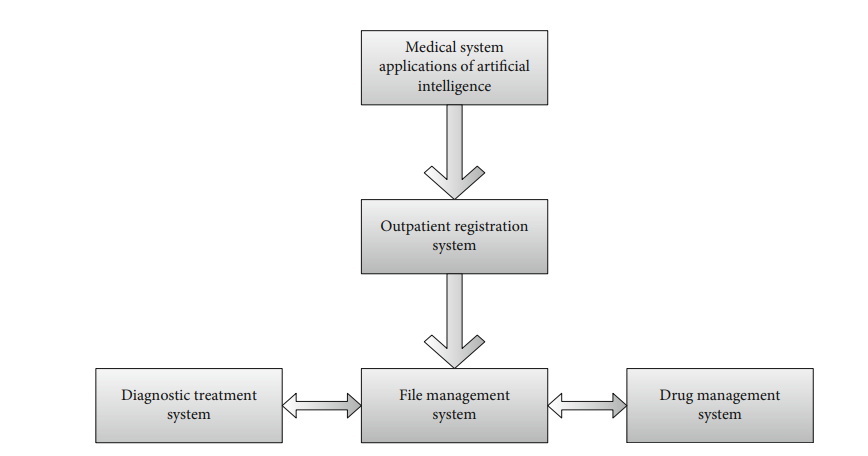
\includegraphics[width=1\textwidth]{imagens/iaSaúde.png}
    \caption{Aplicações da Inteligência Artificial na Saúde \cite{iasaude}.}
    \label{fig:iasaude}
\end{figure}

No contexto do presente trabalho, destaca-se a utilização de algoritmos de \gls{ML} para a realização de diagnósticos prévios de doenças, tais como através da interpretação de imagens médicas, tais como exames de \gls{MRI}, de \Gls{TAC}, radiografias, dados provenientes de Medições quotidianas dos pacientes, dados fisiológicos, bem como de dados elétricos provenientes do funcionamento vital do organismo.

Os estudos ao nível da \gls{IA} na saúde têm evoluído bastante, sendo que através de dados provenientes da última década (2013, 2014, 2015 e 2016) retirado do \textit{PubMed}, se verifica uma evolução ao nível de estudo de Diagnóstico e Terapêutica de diversas doenças (Figura \ref{fig:iasaudedoenças}).

\begin{figure}[H]
    \centering
    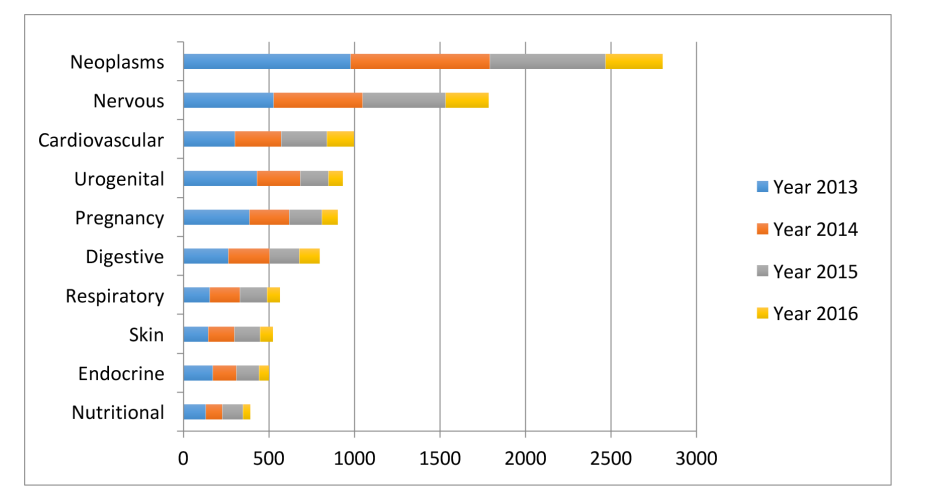
\includegraphics[width=0.8\textwidth]{imagens/iaSaúdeDoenças.png}
    \caption{Quantidade de estudos por Doença na Saúde através da aplicação de \gls{IA} \cite{Jiang230}.}
    \label{fig:iasaudedoenças}
\end{figure}

Da Figura \ref{fig:iasaudedoenças}, verifica-se que o Estudo do sistema nervoso é bastante frequente, sendo que, no presente trabalho o estudo é relativo a uma doença neurodegenerativa (Doença de Parkinson), pertencente ao Sistema Nervoso.

A \gls{DP} é a segunda doença neurodegenerativa mais presente, apenas sendo superada pela doença de \textit{Alzheimer}, e sendo esta doença com uma maior incidência em pessoas com uma idade mais avançada (raramente acontece antes dos 50 anos), à medida que a população mundial envelhece a sua prevalência aumenta de forma diretamente proporcional. Atualmente, verifica-se que a estimativa de existência de pessoas diagnosticadas com a Doença de \textit{Parkinson} é de um valor de entre os 7 a 10 milhões de pessoas \cite{ferreiraPortugal}. No contexto nacional, a Doença também se tem prosperado, sendo que em Portugal, num estudo publicado no ano de 2017, se estima uma existência dr 180 casos em cada 100 mil habitantes, resultando numa estimativa total de 18 a 20 mil pessoas \cite{spn2024}.

Apesar de a sua causa ainda continuar desconhecida, variados estudo têm sido feito acerca dos efeitos do Sistema Nervoso central \cite{Cabreira_Massano_2019}. Na sua origem está uma perturbação crónica do Sistema Nervoso Central, onde os neurónios dopaminérgicos, que apresentam a função de realizar a produção de dopamina são afetados, sendo a dopamina um neurotransmissor associados a funções de movimento e memória. Trata-se de uma Doença progressiva, que não apresenta cura onde o indivíduo acaba por atingir um estado de dependência dos demais, uma vez que apresenta diversas consequências motoras, tais como perda da função muscular que resulta em bradicinesia (lentidão
movimento), rigidez dos membros, postura prejudicada e problemas de marcha e equilíbrio. Contudo. também existem sintomas não-motores que se podem manifestar nas diversas etapas da Doença, tais como depressão, ansiedade e demência \cite{Cabreira_Massano_2019} \cite{silviadeldin}.


Apesar de não existir uma cura para a Doença de \textit{Parkinson}, e esta se encontrar longe de ser uma possibilidade, vários esforços têm sido realizados ao nível da Indústria Farmacêutica, bem como ao nível de Cirurgias, com a intenção de reduzir os seus sintomas, promovendo um melhor estilo de vida.
No que concerne ao tratamento da Doença de \textit{Parkinson}, não existe um método que possa ser extrapolado e generalizado em todos os portadores da doença. Desta forma, geralmente o tratamento varia de indivíduo para indivíduo, sendo diferente, personalizado e característico de cada utente, bem como diferente para os vários estágios da doença. Apesar deste pressuposto, um frequente primeiro contexto da prática do tratamento é a utilização de um Medicamento \gls{L-Dopa}, que tem por objetivo o retardamento da progressão dos efeitos motores que envolve a doença, através da redução rápida de sintomas como Tremores e rigidez muscular.


Atualmente, o Diagnóstico mais utilizado é a visualização do desempenho motor do paciente, contudo, acredita-se sempre que um diagnóstico mais prévio da Doença de \textit{Parkinson} permita uma maior previsão do tratamento eficaz, bem como uma melhor capacidade de tratamento do utente. Posto isto, torna-se necessário o investimento em sistema que permitam um diagnóstico prévio da Doença de \textit{Parkinson}.

Contudo para este processo de diagnóstico de doença ser efetivo é necessário um processo de \textit{Machine Learning} intenso, uma vez que os dados na área de medicina são frequentemente poucos e bastante desbalanceados.


\section{Motivação e objetivos principais}

Em 2015, estudos reportaram que cerca de 177000 pessoas morreram com a doença de \textit{Parkinson}, devido a uma diminuição de diagnóstico prévios efetivos, sendo esta a segunda doença neurodegenerativa que causa mais complicações \cite{20161545}. Tendo isto em conta, o diagnóstico e prognóstico da doença nas suas fases mais prévias é de tremenda importâncias, uma vez que permite um melhor tratamento da mesma.

Através da Literatura, verifica-se que cerca de 90\% dos pacientes apresentar alteração ao nível da fala nas fases mais prévias da Doença de \textit{Parkinson}, sendo assim um dos principais sintomas que pode ser utilizado como diagnóstico.

Sabe-se que não existe nenhuma forma efetiva de realizar o diagnóstico da doença de \textit{Parkinson}, contudo através de diversas pesquisar feitas por investigadores, têm-se realizado diversas abordagens com o intuito de promover este diagnóstico.  Algoritmos de \textit{Machine Learning} tem sido bastante utilizados por investigadores na Área da Medicina e de Biomédica, como alternativa ou como método de apoio ao diagnóstico e tratamento de doenças, uma vez que este podem ser utilizados para a classificação do doenças e apresentam resultados precisos e confiáveis.

Posto isto e tendo em conta os pressupostos definidos nos parágrafos prévios, a principal motivação da presente dissertação passa pelo estudo da possibilidade da realização de um diagnóstico prévio da Doença de Parkinson através de um conjunto de dados da fala, recorrendo a algoritmos de \textit{Machine Learning}. No que concerne ao processo em si, tem-se como objetivo a realização do levantamento do estado de arte relativo a projetos em que se utilizou o mesmo dataset com o mesmo objetivo, bem como o processo em si e os algoritmos utilizados. Ainda neste sentido pretende-se a elaboração de um processo que englobe a análise dos dados existentes, avaliação dos dados e do desbalanceamento existe, pré-processamento dos dados, bem como o processo da seleção das melhores \textit{features}. Espera-se ainda a utilização de diversos Modelos de \textit{Machine learning}, bem como a respetiva otimização.


\section{Metodologia de Investigação}

Durante o processo de desenvolvimento do presente trabalho, optou-se por uma estrutura de trabalho denominada por \gls{CRISP-DM}.

Este tipo de metodologia, é usualmente utilizada em contexto profissional, sendo vista como a abordagem mais comum aos diversos problemas, que podem ser resolvidos através de \emph{Data Mining}.

Neste sentido, o \gls{CRISP-DM} assenta em 6 fases, das quais se destacam:

\begin{itemize} 
\itemsep-0.5em 
    \item Business Understanding; 
    \item Data Understanding;
    \item Data Preparation;
    \item Modeling; 
    \item Evaluation;
    \item Deployment.
\end{itemize}

\section{Estrutura do Documento}

A estrutura do presente Documento assenta na utilização de 5 diferentes capítulos, sendo estes capítulos denominados como "Introdução", "A Doença de \textit{Parkinson}", "\textit{Machine Learning}", "O Caso de estudo" e "Conclusão e Trabalho Futuro", respetivamente.

O presente capítulo é a Introdução, onde se faz uma contextualização do problema que se estuda ao longo do projeto, bem como apresenta os contextos da motivação e a metodologia utilizada.

No segundo capítulo, "A Doença de \textit{Parkinson}", apresenta-se uma explicação do estudo efetuado desta doença, nomeadamente os seus fundamentos, causas, principais sintomas, bem como meios de diagnóstico e tratamento. Ainda neste capítulo apresenta-se uma revisão Bibliográfica da Doença, mais concretamente acerca de trabalhos em que se utilizou fundamentos de \gls{ML} para o diagnóstico da \gls{DP}, mais concretamente em Métodos estatísticos e de \gls{ML} utilizados no conjunto de dados utilizado no presente trabalho.

No Terceiro Capítulo contextualiza-se fundamentos Teóricos de \textit{Machine Learning}, dando-se um contexto dos diferentes tipos de Aprendizagem diferentes, bem como as suas principais aplicações. Ainda neste capítulo, estrutura-se as diferentes fases de um processo de \textit{Machine Learning}, bem como o que se realiza em cada uma destas fases. Por último, apresentam-se fundamentos teóricos e explicações acerca dos diferentes métodos e técnicas de Preparação dos dados, bem como o seu intuito. Procede-se com o mesmo para os Algoritmos e Métricas de Aprendizagem Supervisionada.

No Quarto capítulo, denominada como "O Caso de Estudo", apresenta-se e descreve-se o caso de estudo, os dados utilizados e onde se faz uma análise aos resultados obtidos dos diferentes métodos utilizados: conjunto de dados completo e conjunto de dados dividido por género. Ainda neste capítulo faz-se a análise a diversos algoritmos e a diversos métodos de seleção de \textit{features}.

No último capítulo, procede-se com as conclusões finais desta dissertação, a apresentação de limitações do trabalho desenvolvido, mas também se apresentou sugestões de melhorias futuras ao presente trabalho.



\chapter{A Doença de \textit{Parkinson}}

Este capítulo é uma introdução à doença de \textit{Parkinson}, bem como as suas causas, sintomas e possíveis tratamentos associados.

\section{Fundamentos da Doença de \textit{Parkinson}}

A Doença de \textit{Parkinson} foi descrita pela primeira vez no ano de 1817 por um Cirurgião Inglês de seu nome \textit{James Parkinson}, no seu estudo denominado por "\textit{An Essay on the Shaking Palsy}". Neste estudo, descreve a doença como uma espécie de paralisia agitante \cite{Donaldson2015}. Devido à importância deste estudo, Jean-Martin Charcot, um neurologista Francês, em homenagem ao estudo supramencionado, deu o seu nome à Doença \cite{Parent2018}.

Atualmente, A Doença de \textit{Parkinson} é a segunda doença neurodegenerativa mais comum, sendo que apenas é superada pela Doença de \textit{Alzheimer} \cite{Cabreira_Massano_2019}. Além de ser uma doença neurodegenerativa crónica, também é uma doença progressiva que piora ao longo do tempo de vida, que afeta principalmente o sistema motor. Esta doença é caracterizada por tremores, rigidez muscular, lentidão de movimentos e instabilidade postural.  

No que concerne á Epidemiologia associada à Doença, verifica-se que esta apresenta alterações consoantes a localização geográfica. Estima-se que no Continente Europeu exista entre 257 e 1400 casos por cada 100 mil habitantes, enquanto que no conceito nacional, verifica-se que em Portugal, numa amostra populacional com indivíduos acima dos 50 anos de idade, existe uma prevalência da Doença de \textit{Parkinson} de 180/100000 habitantes, onde existe uma pico por voltas dos 70 anos com uma proporção mais prevalentes nos homens em relação ás mulheres (3:2) \cite{Cabreira_Massano_2019}.

Como a doença de \textit{Parkinson} é progressiva e crónica, o que significa que os sintomas tendem a piorar ao longo do tempo e sem cura, torna-se necessário a existência de tratamentos que possam aliviar significativamente os sintomas e melhorar a qualidade de vida dos pacientes.

\section{Causa}

A causa exata da Doença de \textit{Parkinson} ainda não é compreendida na sua totalidade, mas acredita-se que seja uma combinação de fatores genéticos e fatores ligados ao ambiente. Contudo, na sua maioria, os casos de doença de \textit{Parkinson} existentes ocorrem de forma esporádica, isto é, não estão diretamente ligados a fatores genéticos ou ambientais conclusivos.

Aliado ao fator genético, verifica-se que a doença de \textit{Parkinson} tem uma prevalência maior em adultos acima dos 50 anos e que geralmente é mais comum em homens do que em mulheres e que a progressão da doença pode ser mais lenta nas mulheres, comparativamente com os homens.  \cite{GILLIES2014370}.

Apesar da sua origem ainda ser incerta, a fisiopatologia da doença de \textit{Parkinson} tem sido bastante estudada e é uma doença que integra o grupo das sinucleinopatias, associada com a acumulação da proteína alfa-sinucleína de forma anómala no tecido neuronal, o que resulta num complexo denominado pro "\textit{Lewy Bodies}", que está associado aos sinais neuro-imagiológicos do processo de Morte neuronal, isto é, das células nervosas. Este processo de morte neuronal compreende a degeneração progressiva de células nervosas na parte do cérebro que controla o movimento, conhecida como substância negra. A Substância negra liberta Dopamina, que atua como mensageira entre partes do sistema nervoso e o cérebro para coordenar os movimentos e a regulação do humor. A quantidade de Dopamina no cérebro diminui se essas células nervosas morrem. Isto indica que a região do cérebro que controla o movimento não está funcionando tão bem como deveria, resultando em movimentos lentos e irregulares \cite{Dopamina}. A Substância Negra, bem como o seu efeito, pode ser visualizado na Figura \ref{fig:Substância Negra}.

\begin{figure}[H]
    \centering
    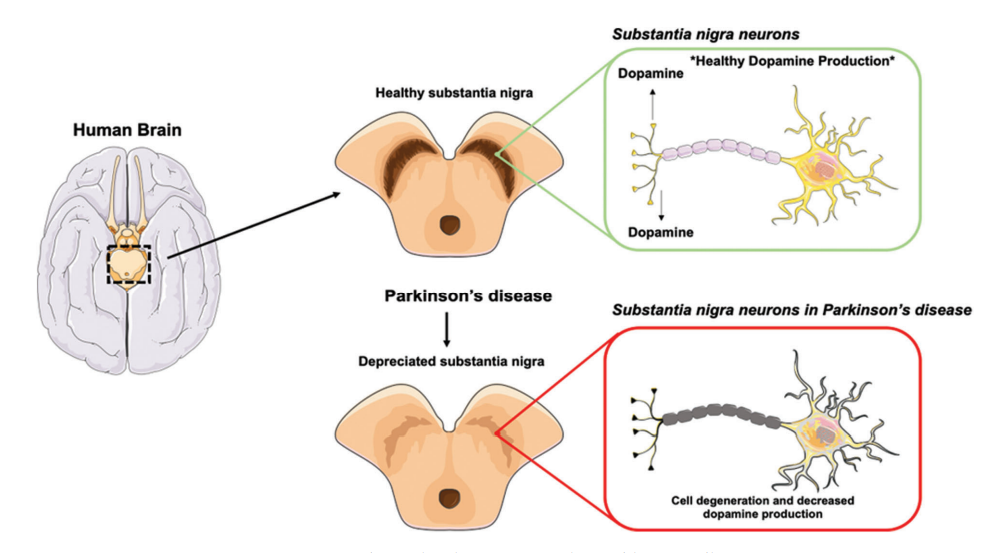
\includegraphics[width=0.8\textwidth]{imagens/Substância Negra.png}
    \caption{Substância Negra \cite{Dopamina}.}
    \label{fig:Substância Negra}
\end{figure}

Tendo em conta que esta doença é progressiva e que a sua causa exata ainda é uma incógnita, torna-se necessário os estudos de várias formas de possível diagnóstico, com o intuito de se realizar um tratamento mais eficaz, possibilitando a prevenção e retardamento do progresso da doença.

\section{Sintomas}

Apesar de a Doença de \textit{Parkinson} ser muito associado com manifestações motoras, estes não são os únicos sintomas, bem como as únicas consequências desta doença, uma vez que existem consequências não motoras \cite{Jankovic368}. Usualmente, tremores em repouso, bradicinesia (movimentos lentos), rigidez e perda de reflexos ao nível de postura são geralmente considerados os sinais mais característico da Doença de \textit{Parkinson}, e os mais associados com as manifestações da Doença, contudo a identificação de Sintomas não motores permite também uma melhoria nos cuidados clínicos prestados, monitorização da doença bem como uma melhor compreensão do seu estado evolutivo \cite{Cabreira_Massano_2019}.

Os sintomas da doença de \textit{Parkinson} podem variar de pessoa para pessoa e podem se manifestar de maneira gradual. Eles geralmente começam de forma leve e pioram com o tempo à medida que a degeneração das células nervosas no cérebro progride. Os principais sintomas estão presentes na Tabela \ref{tab:numeros}, onde se faz uma distinção entre Sintomas Motores e Sintomas Não Motores.

\begin{table}[h]
\small
\caption{Sintomas da Doença de \textit{Parkinson}}
\label{tab:numeros}
\centering
\begin{tabular}{c c}
\hline
\textbf{Sintomas Motores} & \textbf{Sintomas Não Motores} \\ 
\hline
Tremores & Distúrbios do Sono \\ 
Rigidez Muscular  &  Depressão e Ansiedade \\ 
Bradicinesia  &   Diminuição da Capacidade Cognitiva\\ 
Instabilidade Postural  & Psicose\\ 
Dificuldade na Marcha   & Apatia\\ 
Alterações na Coordenação Motora & Fadiga    \\
Alterações na fala    \\
\end{tabular}
\end{table}

Os Sintomas Motores e Não Motores são descritos nos próximos parágrafos:

\begin{description}
  \item[Tremores:] Tremores involuntários, geralmente começando em uma das mãos quando está em repouso é o sintoma mais comum e mais facilmente reconhecível. Estes tremores são unilaterais, involuntários, rítmicos e geralmente ocorrem a uma frequência entre 4 e 6 Hz \cite{Cabreira_Massano_2019}.
  \item[Rigidez Muscular:] A Rigidez Muscular verifica-se pelo aumento da resistência durante o movimentos dos membros e do pescoço, associados a um fenómenos de dor, levando a desconforto e dificuldade de movimento. Este sintoma, normalmente é avaliado pelos médicos através do movimento passivo dos membros dos pacientes.
  \item[Bradicinesia:] Refere-se à progressiva lentidão de movimentos e redução da amplitude de movimentos alternados e repetitivos (abrir e fechar da mão, oponência do polegar e indicador, pronação-supinação das mãos ou mesmo o bater repetitivo do calcanhar no chão) \cite{Cabreira_Massano_2019}. Pode tornar as atividades diárias, como se vestir ou comer, mais demoradas.
  \item[Instabilidade Postural:] Este sintoma é um dos mais tardios a ser manifestado, e  apresenta-se como a dificuldade em manter o equilíbrio e a postura, o que pode aumentar o risco de quedas.
  \item[Dificuldade na Marcha:] Pode ocorrer um padrão de caminhar arrastado, com passos curtos e uma postura inclinada para frente.
  \item[Alterações na Coordenação Motora:] Dificuldade em realizar movimentos coordenados e precisos. Em indivíduos com Doença de \textit{Parkinson} a postura é um pouco fletida \cite{Cabreira_Massano_2019}.
  \item[Alterações na fala:] A fala pode tornar-se mais lenta e menos articulada. Caracterizada por uma voz rouca, de volume reduzido, variabilidade de tom restrita (monótono), articulação imprecisa (fala arrastada) e taxa de fala instável.
  \item[Alterações do Sono:] Pessoas com \textit{Parkinson} podem ter dificuldades em conciliar o sono, apresentar movimentos involuntários durante o sono ou experienciar sonhos vividos.
  \item[Depressão e Ansiedade:] Estes sintomas podem variar bastante de acordo com a gravidade dos sintomas.
  \item[Diminuição da Capacidade Cognitiva:] Este fenómeno verifica-se particularmente em casos em que a Doença de \textit{Parkinson} se encontra mais avançadas ou mesmo no caso de pessoas mais idosas. Neste sintoma, verifica-se a limitação ao nível de pensamento, bem como de encontrar as palavras ou o pensamento correto. 
\end{description}

É importante notar que nem todas as pessoas com \textit{Parkinson} experimentam todos esses sintomas, e a gravidade dos sintomas pode variar. Além disso, outros sintomas não relacionados ao movimento podem ocorrer, como alterações cognitivas, depressão, ansiedade e problemas de olfato.


\section{Diagnóstico e Tratamento}
Apesar de atualmente não existir um teste ou biomarcador definitivo na Doença de \textit{Parkinson}, este pode ser de forma obtido de forma confiável através da examinação de um Neurologista que esteja treinado no diagnóstico e tratamento de Doenças Neurológicas

O diagnóstico da doença de \textit{Parkinson} é geralmente feito com base na avaliação clínica dos sintomas pelo médico, através de um questionários ao paciente, bem como uma observação neurológica detalhada.

O tratamento visa aliviar os sintomas e melhorar a qualidade de vida do paciente, muitas vezes envolvendo medicamentos, terapia física e ocupacional, e, em alguns casos, cirurgias como a estimulação cerebral profunda.

No que diz respeito ao tratamento da Doença de \textit{Parkinson}, a utilização de medicamentos dopaminérgicos são a base da
terapia sintomática para sintomas motores na doença de \textit{Parkinson} \cite{Kobylecki393}.

Após a sua descoberta, a levodopa foi o primeiro tratamento sintomático para a doença de \textit{Parkinson}, seguida pela utilização de agonistas da dopamina e inibidores da monoamina oxidase B \cite{Kobylecki393}. A utilização de agonistas da dopamina, que atuam nos receptores de dopamina no corpo estriado, inibidores da monoamina oxidase B e/ou inibidores da catecol-o-metil-transferase têm como intuito a prevenção da degradação periférica da levodopa \cite{Kobylecki393}.

A levodopa, também conhecida como  L-DOPA, é um precursor natural da dopamina, ou seja, a dopamina é produzida a partir da levodopa no cérebro, um neurotransmissor no cérebro que desempenha um papel fundamental no controlo do movimento, na tentativa de reverter a diminuição da produção de dopamina consequente da doença de \textit{Parkinson}. Para a obtenção de dopamina, a levodopa, após a passagem da barreira hematoencefálica, entra no cérebro, onde é convertida em dopamina \cite{Kobylecki393}\cite{https://doi.org/10.1111/joim.13541}.

Por outro lado, "\textit{Deep brain stimulation}" é um tipo de terapia mais invasiva, terapia sintomática neuro-cirúrgica segura para pacientes elegíveis com doença avançada, especialmente em casos em que os sintomas não respondem adequadamente aos medicamentos dopaminérgicos ou quando os efeitos colaterais dos medicamentos tornam-se problemáticos. \cite{https://doi.org/10.1111/joim.13541}.

A \gls{DBS} consiste na implantação de elétrodos extremamente finos em áreas específicas do cérebro, elétrodos estes que são conectados a um neuro-estimulador, que é colocado sob a pele na região do peito ou na parede abdominal. Este dispositivo gera impulsos elétricos que ajudam a modular a atividade neural nas áreas-alvo, proporcionando alívio dos sintomas motores associados à doença de \textit{Parkinson} \cite{https://doi.org/10.1111/joim.13541}. A título de exemplo, na Figura \ref{fig:dbs}, mostra-se a zona específica da colocação dos elétrodos.

\begin{figure}[H]
    \centering
    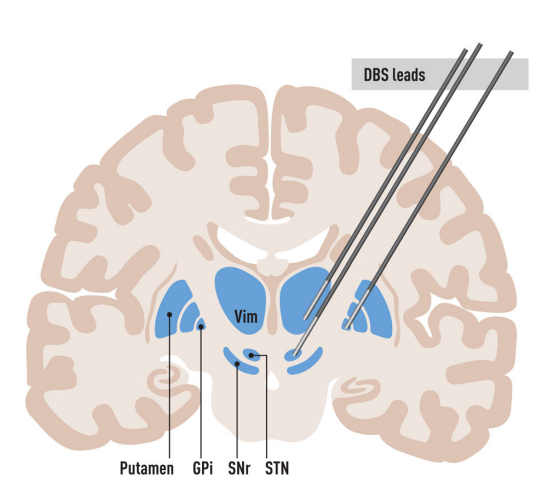
\includegraphics[width=0.6\textwidth]{imagens/DeepBrainStimulation.png}
    \caption{Colocação dos Elétrodos na \gls{DBS}.}
    \label{fig:dbs}
\end{figure}


\section{Estudos Prévios}

O diagnóstico automático da \gls{DP} tem despertado o interesse de muitos como uma forma de permitir um diagnóstico mais preciso e eficiente da \gls{DP}, ao mesmo tempo que reduz a carga de trabalho dos profissionais médicos. Neste sentido, diversos domínios de deteção têm sido utilizados de forma a tentar realizar uma deteção prévia, tais como a deteção a partir de postura/movimento através do uso de \textit{wearable systems}, sistemas de deteção a partir da voz, desenho e escrita, bem como através de sistemas de processsamento de imagem médica.

Estudos recentes demonstraram que existem anormalidades na fala, que podem ser utilizadas como um indicador quantificável para o Diagnóstico automático e precoce da Doença de \textit{Parkinson}. Nos estágios iniciais da \gls{DP}, a maioria das pessoas apresenta problemas vocais. Os sinais de voz são sinais oscilatórios não lineares e não estacionários. Como cerca de 90\% dos pacientes apresentam anomalias vocais no início da progressão da doença, esses sintomas podem ser úteis na deteção da doença \cite{diagnostics12123000}.

Mostafa et al.\cite{MOSTAFA201990} utilizaram um sistema multiagente para selecionar 11 recursos dos 23 recursos, no seu conjunto de dados. Uma vez realizada a etapa de processamento de dados, utilizaram diversos algoritmo para o treino e teste: \gls{DT}, \gls{NB}, \gls{MLP}, \Gls{RF} e \Gls{SVM}, antes e após a aplicação do sistema multiagente de seleção de recursos. Na etapa de testes utilizou-se um \textit{Cross-Validation} com 10 \textit{folds}. A nível de resultados mostraram que a utilização do Sistema multiagente para seleção de \textit{features} melhorou a performance dos modelos, uma vez que permitiu uma melhor seleção do conjunto de \textit{features}. No conjunto de dados final, ou seja, após a seleção das \textit{features}, obtiveram-se valores acima de 89\% de \textit{accuracy} em todos os modelos, sendo que este valor em média foi cerca de 10\% superior quando comparado com o conjunto de dados inicial, tal como pode ser verificado na Figura \ref{fig:mustafa}. 

\begin{figure}[H]
    \centering
    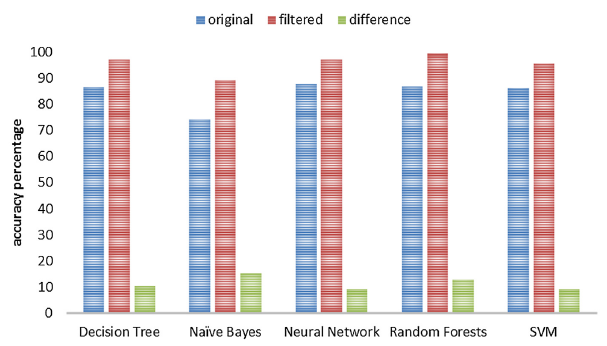
\includegraphics[width=0.8\textwidth]{imagens/mustafaresults.png}
    \caption{Resultados apresentados no estudo \cite{MOSTAFA201990}.}
    \label{fig:mustafa}
\end{figure}

Posto isto, a nível de performance o \textit{Naive Bayes} foi o que aumentou mais a sua performance tendo em conta a comparação entre conjunto de dados original e conjunto de dados com seleção de features, no entanto o algoritmo que apresentou melhores resultados foi o \textit{Random Forest}, com uma \textit{accuracy} de 99,492\%.

Sakar et al. \cite{SAKAR2019255} apresentaram um estudo metódico de processamento de sinais de voz para a deteção da doença de \textit{Parkinson}. Os autores extraíram recursos de sinais de voz de 252 paciente, sendo estes pacientes com ou pacientes sem \gls{DP} usando \gls{TQWT}. Os autores concluíram que o desempenho da utilização de \gls{TQWT} é superior a outras abordagens de processamento de sinais de voz de ponta que são utilizado na classificação da doença de \textit{Parkinson}. Neste estudo, \textit{subsets} de \textit{features} são utilizadas como \textit{inputs} de classificadores múltiplos, sendo as previsões destes classificadores utilizadas como \textit{input} do método \textit{Ensemble}.

Neste estudo, na etapa de Pré-processamento, procedeu-se a uma estandardização dos dados, sendo que posteriormente procedeu-se com a seleção das \textit{features} através de \gls{mRMR}, onde se obtiveram as features mais relevantes e permitiu a redução da dimensionalidade do problema. Uma vez obtidas as features finais, procedeu-se à utilização de diversos métodos de classificação, dos quais as previsões foram o input de métodos de \textit{Ensemble Voting} e \textit{Ensemble Stacking}.

Şule Yücelbaş \cite{yucelbaslogistic} devido à prevalência da Doença de \textit{Parkinson} ser superior nos indivíduos do sexo Masculino, propôs a utilização de um \textit{Simple Logistic Hybrid System Based on Greedy
Stepwise Search Algorithm (SLGS)}, que através da análise de features (redução para o número de \textit{features} mínimo possível) permite a identificação da Doença de \textit{Parkinson}, por género. As etapas do sistema proposto estão presenta na Figura \ref{fig:yucelbaslogistic}.

\begin{figure}[H]
    \centering
    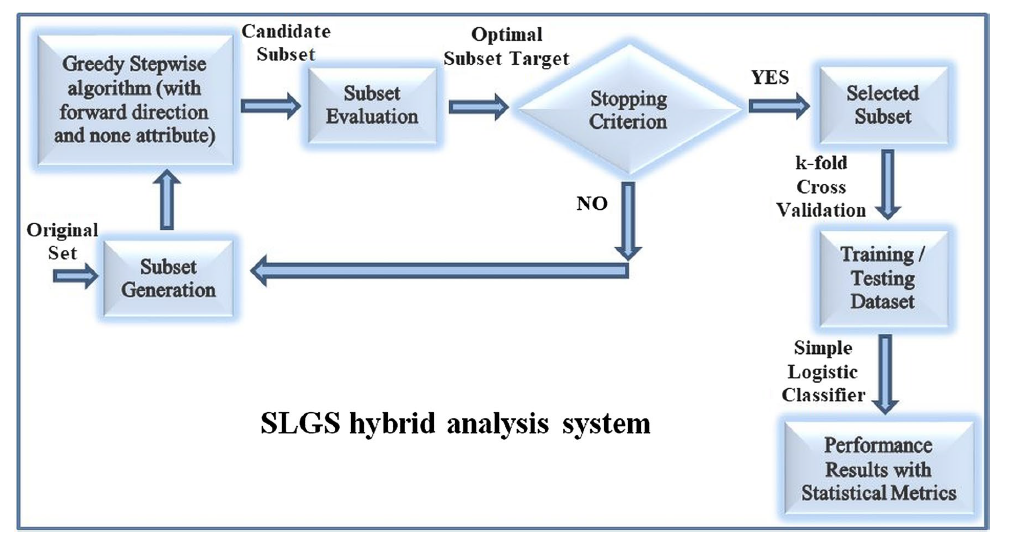
\includegraphics[width=0.8\textwidth]{imagens/yucelbaslogistic.png}
    \caption{Sistema proposto para a classificação de \textit{Parkinson}, por género \cite{yucelbaslogistic}.}
    \label{fig:yucelbaslogistic}
\end{figure}

No que concerne aos resultados apresentados, o sistema através da utilização de 11 features foi capaz de realizar a deteção no sexo Masculino com uma \textit{accuracy} de 88,71\%, enquanto que no sexo Feminino, com 9 features foi capaz de realizar a classificação com uma \textit{accuracy} de 87,15\%.

Tuncer et al. \cite{Tuncer2020} utilizaram o conjunto de dados com 753 características da voz, retirado do repositório público de \textit{UCI Machine Learning Database}. Como consideram que o \textit{dataset} é pequeno, decidiram-se pela utilização de métodos de \textit{Machine Learning} não convencionais, isto é \textit{MAMa tree} é utilizada no conjunto de dados proveniente, de forma a extrair as \textit{features}, sendo que os dados presentes nos diferentes nodos são combinados, sendo posteriormente utilizado um \gls{SVD} feature extraction para a seleção de \textit{features}. Na fase de seleção de \textit{features}, 122 \textit{features} são referidas, sendo das quais 50 são extraídas como as mais importantes, usando seleção de \textit{features} através de \textit{relief}. Posteriormente, 8 algoritmos de classificação (\gls{LD}), \gls{SVM} linear, \Gls{SVM} com \textit{kernel} de \gls{RBF}, e \textit{kernel} cúbico, \gls{LR}, \gls{NN} \textit{with city block distance and k = 1}, e \gls{BT}) são utilizados em 2 casos:
\begin{itemize}
    \item Caso 1: Pré-processamento, Extração de features e Classificação.
    \item Caso 2: Pré-processamento, Extração de features, Classificação e etapa de pós-processamento.
\end{itemize}

Ao nível de resultados, no caso 1, o resultado superior foi uma \textit{accuracy} de 92,46\%, enquanto que no caso 2 foi uma \textit{accuracy} de 96,83\%, ambos através da utilização do \gls{NN}.

Nissar, Rizvi, Masood, e Mir \cite{nissaretall} procederam à análise de um estudo no qual se utilizou um conjunto de dados retirado da UCI Machine Learning Database (UCI Machine Learning Repository, 2018). 

Este conjunto de dados é constituído por dados de pacientes normais e por dados de pacientes com doença de \textit{Parkison}. Apresenta 756 registos e 753 características, especialmente utilizadas para classificação
da doença de \textit{Parkinson} através da voz. No seguinte artigo, descreveram o trabalho propostos nas etapas de aquisição de dados, pré-processamento de dados através da normalização dos mesmos através de \textit{Min-Max Scalling},  seleção de \textit{features} mais relevantes através de dois métodos (\textit{Recursive feature selection} e \textit{minimum redundancy}), aplicação de Modelos de \textit{Machine Learning} e avaliação da performance do mesmo. Para a aplicação de Modelos utilizaram-se 9 algoritmos distintos: \gls{NB}, \gls{LR}, \gls{NN}, \Gls{MLP}, \gls{RF}, \Gls{SVM} (linear), \Gls{SVM} (rbf) e \gls{XGBoost} de 3 formas distintas:

\begin{itemize} 
\itemsep-0.5em 
    \item Seleção de características com a técnica \textit{Recursive feature selection} e \textit{minimum redundancy feature selection}, exceto o grupo de características \textit{TWQT}.
    \item Seleção de características com a técnica \textit{Recursive feature selection} e \textit{minimum redundancy feature selection}, exceto o grupo de características \textit{MCFF}. 
    \item Técnicas de seleção de características \textit{Recursive feature selection} e \textit{minimum redundancy feature selection} com todos os grupos de características.
\end{itemize}

Comparando todos os resultados das 3 formas distintas, verificou-se que o algoritmo que obteve melhores resultados foi o \gls{XGBoost}, com uma precisão de 95.39\%, quando utilizada a técnica de seleção
de características \textit{minimum redundancy feature selection}.

Ashour et al. \cite{9072452} propuseram uma \textit{framework} que fazia a seleção das \textit{features} em dois estágios, permitindo a identificação de pacientes com perda de voz em doentes com \textit{Parkinson}. Os autores afirmar que as 753 características aumentam bastante a dimensão do espaço das \textit{features} e que aumentam a possibilidade de existência de \textit{features} irrelevantes, sendo que processo de seleção de \textit{features} é a melhor maneira de reduzir esta dimensão. Os autores utilizaram métodos de \gls{PCA} e \gls{ECFS} como seleção de \textit{features}, permitindo tirar vantagens de ambos os métodos. Uma vez selecionadas as \textit{features}, utilizou-se como método de classificação o algoritmo de \gls{SVM} com o \textit{kernel} cúbico. A nível de resultados, verificou-se que existiu uma melhoria na \textit{accuracy} com e sem a realização da seleção de \textit{features} proposta, verificando-se um aumento de 88\% para 94\%.

Omar Barukab, Amir Ahmad, Tabrej Khan e Mujeeb Rahiman Thayyil Kunhumuhammed \cite{diagnostics12123000} recorreram a um conjunto de dados
disponibilizado por C. O. Sakar et al. (2019), conjunto de dados que apresenta  756 registos e 753 características, onde 65 dos pacientes são saudáveis (41 do sexo Feminino e 23 do sexo Masculino) e 188 pacientes (81 do sexo Feminino e 107 do sexo Masculino) apresentam doença de \textit{Parkinson}, ou seja, uma dataset desbalanceado. Neste artigo, os autores propõem a utilização de diferentes métodos de \textit{ensemble}, com ou sem a utilização de métodos de \textit{oversampling} ou \textit{undersampling}. Os resultados mostraram que
\textit{AdaBoost}, \gls{RF} e  \gls{DT} apresentam excelentes métricas, tais como precisão, \textit{recall}, \textit{F1-score}, \textit{area under the receiver operating characteristic curve} (AUROC). Utilizaram-se algoritmos de seleção de   features, tais como o Lasso e \textit{Information gain}, de forma a fazer a seleção das 10 melhores \textit{features}. Por fim, o AdaBoost com método de \textit{Information gain} na seleção de \textit{features} é o método de conjunto de melhor desempenho com uma pontuação F1 de 0,903.

Mohammadi et al.\cite{MOHAMMADI2021100079} recorreram a um conjunto de dados disponibilizado por C. O. Sakar et al. (2019), onde afirma que este conjunto tem um tamanho de amostra limitado e recursos desequilibrados. Neste processo fizeram o uso de \textit{autoencoders} para o processo de seleção de \textit{features}. O resultado mostrou que o uso de \textit{autoencoders} como extratores de features pode ser benéfico quando o total de amostras é menor que o número de recursos, especialmente quando a entrada está desequilibrada. 

Uma vez obtido o conjunto de dados, primeiramente realizaram a normalização de todas as \textit{features}, de forma a que estas apresentem todas a mesma escala. Uma vez normalizados os dados, desenvolveram 2 abordagens distintas para o mesmo problema: treino e avaliação com os dados simplesmente normalizados e treino e avaliação com os dados normalizados e com o processo de seleção de features através de \textit{autoencoders}.

Para a primeira maneira, utilizaram-se os modelos de \gls{SVM}, \Gls{XGBoost} e \Gls{MLP} com a utilização de \textit{cross-validation} com 5 \textit{folds} e \textit{tuning} de hiperparâmetros através do \textit{GridSearch}, de onde foram extraídas as métricas de \textit{Accuracy} e \textit{F1-Score}. Neste sentido, obtiveram-se os seguintes resultados na primeira abordagem:  \gls{SVM} com o \textit{kernel} \textit{poly} e o \textit{degree} a 23, obteve-se uma precisão de 94.07\% e um \textit{F1-Score} de 96,08\%, \gls{XGBoost}, obteve uma precisão de 92.19\% e um \textit{F1-Score} de 94.92\%, com os parâmetros: \textit{colsample\_bytree} = 0.35, \textit{n\_estimators} = 325, \textit{max\_depth} = 4, \textit{learning rate} = 0.1, \textit{alpha} = 1e-2, \textit{subsample} = 0.75 e \gls{MLP} obteve-se uma precisão de 90.61\% e um \textit{F1-Score} 93.72\%, com os parâmetros: camada intermédia = 160 e nodos = 25.

Na segunda maneira, utilizaram-se os mesmos modelos, apenas diferindo que após a normalização dos dados ocorreu um processo de seleção de \textit{features} através de \textit{autoencoders}. Por fim, utilizou-se Métodos de \textit{Ensemble} para o aumento do desempenho dos algoritmos. 

A nível de resultados, mostraram que os modelos de classificação tradicionais superam as técnicas de aprendizagem profunda, mostrando desta forma que os Modelos de \textit{Machine Learning} conseguem obter resultados bons em problemas de classificação, quando comparados com modelos de \textit{Deep Learning}. Nos resultados demonstraram que \textit{Ensemble Learning} apresenta um papel fundamental na melhoria da classificação, uma vez que conseguiram \textit{accuracy} entre 95 e 97\% através da utilização de algoritmo como \gls{SVM}, \Gls{XGBoost}, \gls{MLP} seguidos de \textit{autoencoders}.

Qasim et al. \cite{medicina57111217} recorreram a um conjunto de dados
disponibilizado por C. O. Sakar et al. (2019), onde afirma que este conjunto tem um tamanho de amostra limitada e recursos desequilibrado, representando o \textit{Bias} existente nos \textit{datasets} ligados a Medicina. Neste projeto utilizou-se o algoritmo de \gls{SMOTE} para contornar o desbalanceamento existente no \textit{dataset}. Neste contorno de desbalanceamento teve-se como produto final um \textit{dataset} com 564 registos nas duas classes de classificação. De seguida, procederam com a normalização do \textit{dataset} balanceado.

Younis Thanoun and Yaseen \cite{thanoun} propuseram a utilização de 2 técnicas de \textit{Ensemble} para fazer a deteção de doença de \textit{Parkinson} através de Machine Learning: Classificadores \textit{Stacking} e classificadores \textit{Voting}, após o balanceamento do conjunto de dados através de \gls{SMOTE}, tal como se verifica na Figura \ref{fig:thanoun}.

\begin{figure}[H]
    \centering
    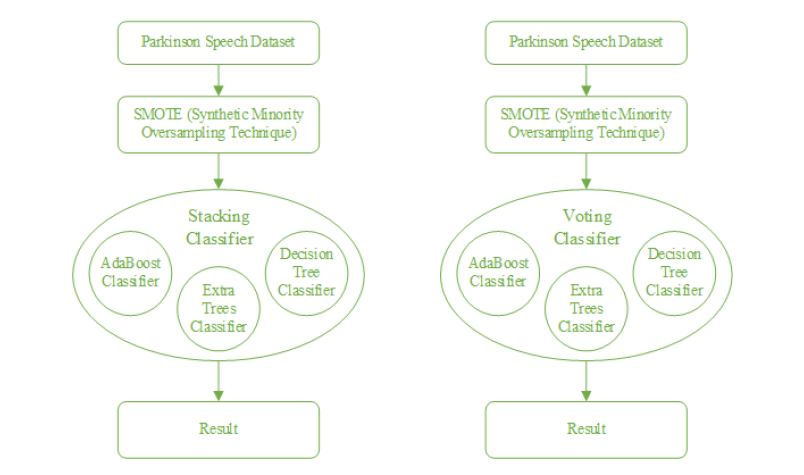
\includegraphics[width=0.7\textwidth]{imagens/thanoun.png}
    \caption{Metodologia apresentada no estudo de Younis Thanoun and Yaseen\cite{thanoun}.}
    \label{fig:thanoun}
\end{figure}

Através dos resultados, verificou-se que os Classificadores \textit{Stacking} apresentaram resultados superiores aos classificadores \textit{Voting}, sendo a \textit{accuracy} de 92,2\% e 83.57\%, respetivamente.

Prasad et al. \cite{Prasad2020}  recorreram a conjunto de dados com 753 \textit{features} da voz, e utilizaram uma framework de classificação em duas etapas, sendo a primeira etapa a utilização de múltiplas \gls{ANOVA} nas features vocais independentes separadamente (MFFCCs, WTs e TQWTs) para seleção de features, que são ligadas com as \textit{Baseline features}, e a segunda etapa a utilização de classificadores \gls{XGBoost}, tal como se verifica na Figura \ref{fig:prasad}. 

\begin{figure}[H]
    \centering
    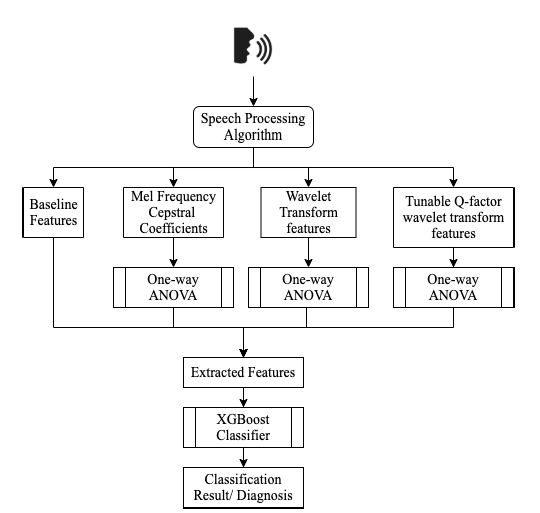
\includegraphics[width=0.6\textwidth]{imagens/prasad.png}
    \caption{Metodologia apresentada no estudo de Prasad et al. \cite{Prasad2020}.}
    \label{fig:prasad}
\end{figure}

No que concerne aos resultados do modelo, a framework proposta apresenta uma \textit{accuracy} de 94,71\% e um \textit{F-1 score} de 0,96.


Uma vez balanceado e normalizado o \textit{dataset} procedeu-se com a seleção das \textit{features}, de forma a evitar contradições existentes, bem como diminuir o tempo de processamento, através de algoritmos de \gls{RFE} e \gls{PCA}. Esta etapa foi bastante importante na redução da quantidade de \textit{features} existentes, uma vez que através do \gls{RFE} fez-se uma redução para exatamente 329 \textit{features}. Após o \gls{RFE}, fez-se novamente uma redução do \textit{dataset} através do \gls{PCA}, o que resultou num valor final de 18 diferentes \textit{features}.

A nível de algoritmos, utilizou-se os seguintes Modelos: \textit{Bagging}, \textit{K-nearest neighbour}, \textit{Multilayer perceptron} e \gls{SVM}. Posteriormente aplicaram métodos de \textit{fine-tuning} através de \textit{GridSearch} obtendo-se os parâmetros presentes na Tabela \ref{tab:optimizacaoqasim}. 

\begin{table}[H]
\small
\caption{Algoritmos utilizados, bem como os parâmetros \cite{medicina57111217}.}
\label{tab:optimizacaoqasim}
\centering
\resizebox{\textwidth}{!}{%
\begin{tabular}{c c}
\hline
\textbf{Algoritmo} & \textbf{Parâmetros do algoritmo} \\ 
\hline
\textit{Bagging} & \textit{Classifier} = \gls{NN}, \textit{Number of iterations} = 100,
\textit{max samples} = 0.9 \\ 
\textit{K-nearest neighbour}  &  \textit{Number of neighbors} = 1, \textit{Leaf size} = 40 \\ 
\textit{Multilayer perceptron}  &   \textit{Number of iterations} = 500, \textit{learning rate} = 0.01, \textit{Solver for optimum
weight} = \textit{adam}\\ 
\gls{SVM}  & \textit{Regularization parameter} = 1, \textit{kernel} = \textit{rbf}, \textit{Gamma} = 2\\ 
\end{tabular}
}
\end{table}

Por último, procederam à avaliação dos algoritmos de 4 formas distintas:

\begin{itemize} 
\itemsep-0.5em 
    \item Conjunto de dados desbalanceado.
    \item Conjunto de dados equilibrado e com a utilização do algoritmo de seleção de \textit{features} \gls{RFE}.
    \item Conjunto de dados equilibrado e com a utilização dos algoritmos de seleção de \textit{features} \gls{RFE} e \gls{PCA}.
    \item Conjunto de dados equilibrado, com a utilização dos algoritmos de seleção de \textit{features} \gls{RFE} e \gls{PCA} e com a utilização do \textit{GridSearch} para otimização.
\end{itemize}

Para a avaliação dos algoritmos foram utilizadas cinco Métricas: \textit{accuracy}, \textit{precision}, \textit{sensitivity}, \textit{specificity}, and \textit{G-Mean}. Por conseguinte, para o primeiro caso o algoritmo que obteve um melhor desempenho foi o \gls{NN} com uma precisão de 87.4\% e com as 753 características do conjunto de dados. No segundo caso o algoritmo que obteve um melhor desempenho foi o \Gls{MLP} com uma precisão de 93.3\% e com 329 características. No terceiro caso, o algoritmo que obteve um melhor desempenho foi também o \gls{MLP} com uma precisão de 95.1\% e com 18 características. Por fim, no quarto
caso foi adicionado o método de \textit{Fine-Tuning} (\textit{GridSearch}) com o objetivo de encontrar os valores ótimos para cada parâmetro dos algoritmos e o algoritmo que teve um melhor desempenho foi o \gls{SVM} com uma precisão de 98\%.

Abdurrahman et al. \cite{Abdurrahman} propuseram a utilização de \gls{XGBoost} para a tarefa de classificação da Doença de \textit{Parkinson}, uma vez que este algoritmo apresenta elevada escalabilidade, ou seja, apresentando uma velocidade de processamento superior e consumo de memória inferior aos algoritmos tradicionais de \textit{Machine Learning}. Ainda neste estudo, seguiu-se a metodologia de trabalho presenta na Figura \ref{fig:abdu}.

\begin{figure}[H]
    \centering
    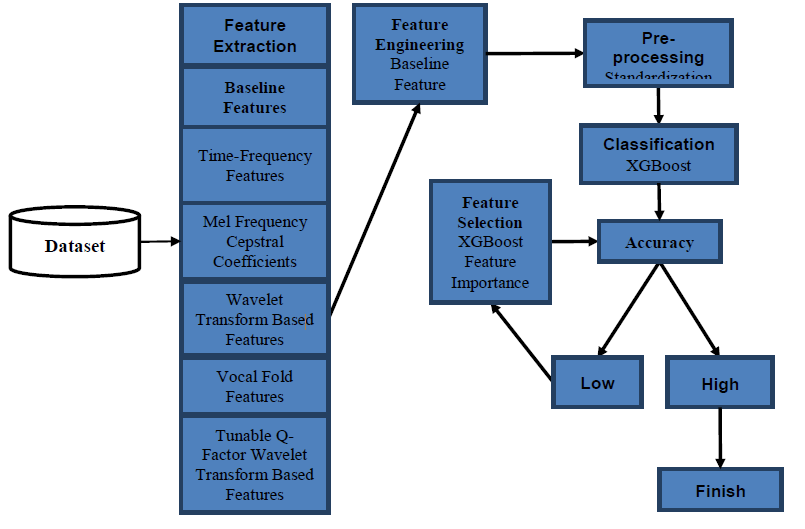
\includegraphics[width=0.7\textwidth]{imagens/abdu.png}
    \caption{Explicação do Processo seguido no estudo de Abdurrahman et al. \cite{Abdurrahman}.}
    \label{fig:abdu}
\end{figure}

Como se pode verificar na Figura \ref{fig:abdu}, partindo de um conjunto de dados com 754 Features, nomeadamente \textit{baseline features, intensity parameters, format frequencies, bandwidth parameters, vocal fold, MFCC, Wavelet Features, }e \textit{TQWT Features}, apenas se procedeu com a utilização das \textit{Baseline features} no estudo.

Na etapa de classificação, apenas se utilizou o algoritmo de \gls{XGBoost}, onde previamente foi realizada a distinção entre conjunto de dados de treino e conjunto de dados de teste, sendo que 33\% dos dados foram selecionados para o conjunto de teste, sendo a restante quantidade selecionada para os dados de treino. Numa primeira fase, o algoritmo de \gls{XGBoost} foi usada para classificação, envolvendo todas as \textit{Baseline Features}, onde se obteve uma \textit{accuracy} de 84.80\%. Posteriormente, utilizou-se a \textit{Feature Importance} do algorimo \gls{XGBoost} para se realizar uma redução no número de \textit{Features}, sendo realizados mais dois testes, um primeiro onde se removeu as \textit{features ddaShimmer} e \textit{locShimmer}, obtendo-se uma \textit{accuracy} de 85.60\%. Num segundo teste, removeu-se as \textit{features locDbShimmer, meanNoiseToHarmHarmonicity, ppq5Jitter,apq5Shimmer, ddpJitter, rapJiter, PPE}, obtendo-se uma \textit{accuracy} de 84.40\%. 

Biswajit Karan1 \cite{Karan2023} propôs a utilização de uma \textit{framework} de \textit{Machine Learning} baseada em duas etapas: seleção de \textit{features} com mais informação através de algoritmo de \gls{XGBoost}, seguida da utilização de algoritmos \textit{ensemble} na etapa de classificação, onde estes algoritmos combinação vários classificadores fracos (\gls{SVM}, \Gls{NN}, \Gls{RF}, \gls{XGBoost} e \gls{MLP}), de forma a criar um classificador mais forte. Nesta etapa, de forma resumida, as probabilidades dos classificadores mais fracos são utilizadas como novas features para diminuir o erro de previsão do classificador principal. Na etapa de treino dos modelos utilizou-se o \gls{LOSO} como técnica de validação cruzada. De forma a classificar a performance dos modelos utilizou-se as métricas de \textit{Accuracy}, sensibilidade, especificadE e \gls{AUC}.

A etapa de seleção de \textit{features} foi realizada com o \gls{XGBoost} variando o valor do \textit{threshold} entre 0.001 e 0.02, onde se obteve o valor ótimo com o \textit{threshold} de 0.009, onde se selecionam 21 \textit{features}, sendo 1 da categoria \textit{Baseline Features}, 4 da categoria de \textit{MFCCs}, 3 da categoria de \textit{DWT-based features} e 13 da categoria \textit{TQWT features}. Estas 21 features foram utilizadas como \textit{features} de entrada da \textit{stack} de métodos \textit{ensemble}. Na etapa de testes de classificadores \textit{ensemble} obteve-se o valor máximo de 95.07\% de accuracy quando se utilizou o \gls{SVM}, \gls{NN}, \gls{RF} e \gls{MLP} como métodos base e o método \gls{XGBoost} utilizado como método de melhoria de performance.

Kemal Polat  \cite{Polat2019} propôs um método híbrido para a deteção da doença de \textit{Parkinson} através da combinação do algoritmo de \gls{SMOTE}, de forma a lidar com o problema de conjunto de dados desbalanceado (192 dados são relativos a utentes sem a doença de \textit{Parkinson}, enquanto que 564 dados pertencem a utentes com a doença de \textit{Parkinson}) conjugado com a utilização de \gls{RF} como algoritmos de classificação. Na etapa de treino e de teste, utilizou-se uma divisão de 50\% de dados para treino e 50\% de dados para teste, com a utilização de \textit{10-fold Cross-Validation}. A nível de resultados, verificou-se que a utilização unitária do método de classificação de \gls{RF}, isto é, sem uma etapa de \gls{SMOTE} apresentou uma \textit{accuracy} de 87,037\%, enquanto que a utilização do método híbrido proposto resultou numa \textit{accuracy} bem superior com o valor de 94.89\%.




\begin{longtable}{|p{6cm}|p{4cm}|p{6cm}|}
\caption{Revisão de Literatura resumida.} \\ \hline
\multicolumn{3}{|c|}{\textbf{Estudos}} \\ \hline
\textbf{Principais Características} & \textbf{Algoritmos} & \textbf{Avaliação do Estudo} \\ \hline
\endfirsthead

\hline
\textbf{Principais Características} & \textbf{Algoritmos} & \textbf{Avaliação do Estudo} \\ \hline
\endhead

Şule Yücelbaş \cite{yucelbaslogistic}:

Conjunto de dados com 753 características da voz, onde se dividiu a classificação por género e procedeu com a seleção de \textit{features} através de \textit{Greedy Stepwise Search Algorithm}.

& \textit{Logistic Regression}

& No que concerne aos resultados apresentados, o sistema através da utilização de 11 features foi capaz de realizar a deteção no sexo Masculino com uma \textit{accuracy} de 88,71\%, enquanto que no sexo Feminino, com 9 features foi capaz de realizar a classificação com uma \textit{accuracy} de 87,15\%. \\ \hline

Tuncer et al. \cite{Tuncer2020}:

Conjunto de dados com 753 características da voz, onde se procedeu com a seleção de \textit{features} através de uma combinação entre \gls{MAMa} e \gls{SVD}.

& \textit{K-Nearest Neighbors with 10-fold Cross-Validation}

& 92,46\% e 96,83\% (com 50 \textit{features}) \\ \hline


Nissar, Rizvi, Masood, e Mir \cite{nissaretall}:
Conjunto de dados com 753 características da voz, onde se aplicou
pré-processamento através da normalização das features entre 0 e 1 e
através de duas diferentes técnicas de seleção de features (\textit{Minimum
redundancy maximum relevance feature selection} e \textit{ Recursive Feature
selection}.
O treino e teste do modelo foi realizado de 3 formas separadas:
-  Seleção de features com a técnica de \textit{Recursive Feature Selection} e
\textit{Minimum redundancy maximum relevance feature selection}, exceto
as \textit{features} de \textit{TWTQ}.
- Seleção de features com a técnica de \textit{Recursive Feature Selection} e
\textit{Minimum redundancy maximum relevance feature selection}, exceto
as features de \textit{MCFF}.
- Seleção de features com a técnica de \textit{Recursive Feature Selection} e
\textit{Minimum redundancy maximum relevance feature selection} com todas as features.
& \gls{NB}, \gls{LR}, \gls{NN}, \gls{MLP}, \gls{RF}, \gls{SVM} (linear), \gls{SVM}(\gls{RBF}) e \gls{XGBoost}.
& - Técnica seleção de características \textit{Recursive feature selection}: o modelo \Gls{XGBoost} tem uma precisão de 95.39\%.
- Técnica seleção de características \gls{mRMR}: o modelo \gls{LR} tem uma precisão de 86,84\%.
- Nas duas técnicas o modelo \gls{SVM} com o \textit{kernel} \gls{RBF} tem uma precisão de 88,15\%. \\ \hline

Younis Thanoun and Yaseen \cite{thanoun} propuseram a utilização de 2 técnicas de \textit{Ensemble} para fazer a deteção de doença de \textit{Parkinson} através de Machine Learning: Classificadores \textit{Stacking} e classificadores \textit{Voting}, após o balanceamento do conjunto de dados através de \gls{SMOTE}.

& Classificadores \textit{Stacking} e classificadores \textit{Voting}, com os algoritmos \textit{AdaBoost, Extra Trees e Decision Tree}.

& Classificadores \textit{Stacking} apresentaram resultados superiores aos classificadores \textit{Voting}, sendo a \textit{accuracy} de 92,2\% e 83.57\%, respetivamente. \\ \hline

Prasad et al. \cite{Prasad2020}  recorreram a conjunto de dados com 753 \textit{features} da voz, e utilizaram uma framework de classificação em duas etapas, sendo a primeira etapa a utilização de múltiplas \gls{ANOVA} nas features vocais independentes separadamente (MFFCCs, WTs e TQWTs) para seleção de features, que são ligadas com as \textit{Baseline features}, e a segunda etapa a utilização de classificadores \gls{XGBoost}, tal como se verifica na Figura \ref{fig:prasad}. 

& \gls{XGBoost}

& No que concerne aos resultados do modelo, a framework proposta apresenta uma \textit{accuracy} de 94.71\% e um \textit{F-1 score} de 0,96. \\ \hline

Ashour et al. \cite{9072452}:
\textit{Framework} que faz a seleção das \textit{features} em dois estágios, permitindo a identificação de pacientes com perda de voz em doentes com \textit{Parkinson}. Os autores afirmar que as 753 características aumentam bastante a dimensão do espaço das \textit{features} e que aumentam a possibilidade de existência de \textit{features} irrelevantes, sendo que processo de seleção de \textit{features} é a melhor maneira de reduzir esta dimensão. Os autores utilizaram métodos de \gls{PCA} e \gls{ECFS} como seleção de \textit{features}, permitindo tirar vantagens de ambos os métodos.

&\gls{SVM} com o \textit{kernel} cúbico. 

&nível de resultados, verificou-se que existiu uma melhoria na \textit{accuracy} com e sem a realização da seleção de \textit{features} proposta, verificando-se um aumento de 88\% para 94\%. \\ \hline

Mohammadi et al.\cite{MOHAMMADI2021100079}
- Conjunto de dados contém 753 registos.
- Pré-processamento dos dados: normalização dos dados
no intervalo [0,1] e técnica de seleção de características
\textit{Autoencoder}.
- Treino e teste dos modelos da seguinte forma:
1. Com todas as características do conjunto de
dados.
2. Apenas com as características selecionadas
pela técnica \textit{Autoencoder}.
- Implementação de \textit{cross validation} com k=5.
- Otimização dos parâmetros através da técnica
\textit{GridSearch}.

& \gls{SVM}, \gls{XGBoost} e \gls{MLP}.
& - Com todas as características do conjunto
de dados o modelo \gls{SVM} tem uma
precisão de 94.07\%.
- Técnica de seleção de
características \textit{Autoencoder}
o modelo \gls{SVM} tem uma precisão
de 91.93%
 \\ \hline

Qasim et al. \cite{medicina57111217}:
Conjunto de dados com 753 registos.
- Pré-processamento: técnica de \textit{SMOTE} para equilibrar o
conjunto de dados, normalização das características no
intervalo [0,1] e aplicação das técnicas de seleção de
características \textit{Recursive feature selection} (selecionou
329) e a \textit{principal component analysis} (18 componentes)
- Divisão do conjunto de dados, num conjunto de dados
de treino 80\% e um conjunto de dados de teste 20\%, com
a validação através da técnica \textit{cross validation}, com k=10.
- Treino e teste dos modelos da seguinte forma:
1. Conjunto de dados desequilibrado;
2. Conjunto de dados equilibrado e técnica de
seleção de características Recursive feature selection;
3. Conjunto de dados equilibrado e as duas
técnicas de seleção de características
\textit{Recursive feature selection} e \textit{Principal Component Analysis};
4. Conjunto de dados equilibrado e as duas
técnicas de seleção de características
\textit{Recursive feature selection} e \textit{Principal
Component Analysis} com os parâmetros
otimizados através da técnica \textit{GridSearch}
& \Gls{MLP}, \gls{SVM}, \gls{NN} e \textit{Bagging}.
& No primeiro caso o modelo \gls{NN} tem uma precisão de 87.4\%.
- No segundo caso o modelo \gls{MLP} tem
uma precisão de 93.3\%.
- No terceiro caso o modelo
\gls{MLP} tem uma precisão 95.1\%
- No quarto caso o modelo
\Gls{SVM} tem
uma precisão de 98\% \\ \hline

Abdurrahman et al. \cite{Abdurrahman}:
Conjunto de dados com 753 características da voz, onde se aplicou
pré-processamento da seleção de apenas as \textit{Baseline Features}
e posteriormente seleção através da \textit{Feature Importance} do Algoritmo de \gls{XGBoost}.
O treino e teste do modelo foi realizado de 3 formas separadas:
- Com todas as Baseline Features.
-  Remoção das features \textit{ddaShimmer} e \textit{locShimmer}.
-  Remoção das features \textit{locDbShimmer, meanNoiseToHarmHarmonicity, ppq5Jitter, apq5Shimmer, ddpJitter, rapJiter} e \textit{PPE}.
& \gls{XGBoost}.
& No primeiro caso obteve-se
uma \textit{accuracy} de 84.80\%.
- No segundo caso obteve-se uma \textit{accuracy} de 85.60\%.
- No terceiro caso obteve-se uma \textit{accuracy} de 84.40\% \\ \hline

Biswajit Karan1 \cite{Karan2023}:
Conjunto de dados com 753 características da voz, onde se aplicou
uma framework de \gls{ML} baseada em duas etapas:
seleção de features com mais informação através de
algoritmo de XGBoost, seguida da utilização de algoritmos
de stacking ensemble na etapa de classificação, onde estes algoritmos
combinação vários classificadores fracos (\Gls{SVM}, \gls{NN}, \gls{RF}, \gls{XGBoost} e \Gls{MLP}).
Na seleção de features, o \textit{threshold} máximo foi conseguido com 0.09
de onde se extrairam 21 \textit{features}.
& \Gls{SVM}, \gls{NN}, \gls{RF}, \gls{XGBoost} e \Gls{MLP}.
& Na etapa de testes de classificadores \textit{ensemble}
obteve-se o valor máximo de 95.07\% de \textit{accuracy}
quando se utilizou o \Gls{SVM}, \gls{NN}, \gls{RF} e \Gls{MLP}
como métodos base e o método \gls{XGBoost} utilizado como método
de melhoria de performance. \\ \hline

Kemal Polat  \cite{Polat2019} :
Propôs um método híbrido para a deteção da doença de \textit{Parkinson} através da combinação do algoritmo de \gls{SMOTE}, de forma a lidar com o problema de conjunto de dados desbalanceado (192 dados são relativos a utentes sem a doença de \textit{Parkinson}, enquanto que 564 dados pertencem a utentes com a doença de \textit{Parkinson}) conjugado com a utilização de \gls{RF} como algoritmos de classificação. Na etapa de treino e de teste, utilizou-se uma divisão de 50\% de dados para treino e 50\% de dados para teste, com a utilização de \textit{10-fold Cross-Validation}. 
& \gls{RF}
& A nível de resultados, verificou-se que a utilização unitária do método de classificação de \gls{RF}, isto é, sem uma etapa de \gls{SMOTE} apresentou uma \textit{accuracy} de 87,037\%, enquanto que a utilização do método híbrido proposto resultou numa \textit{accuracy} bem superior com o valor de 94.89\%. \\ \hline
\end{longtable}


\chapter{Data Mining e Machine Learning}

\section{Machine Learning}
Machine Learning é uma área da Inteligência Artificial que tem como intuito o uso de dados e algoritmo de computação que pretende a imitação do pensamento humano, aumentando a sua performance desta forma\cite{books/daglib/0033642}. Ainda assim, o objetivo passa pela criação e utilização de modelos, de forma a retirar conhecimento de um conjunto de dados\cite{Grus15}.

De forma a se proceder à obtenção de conhecimento, estes modelos utilizam conceito da Matemática, tais como Álgebra Linear, de Estatística e de Probabilidades\cite{Grus15}. Através destes modelos, temos um resultado, que incorpora a previsão ou classificação de um determinado domínio. 

Existem 4 diferentes tipos de Algoritmos de Machine Learning: \gls{SL}, \gls{UL}, Semi-supervised Learning e \Gls{RL}, tal como pode ser visualizado na Figura \ref{fig:tipoAprendizagem} \cite{10.1007/s42979-021-00592-x}. 

\begin{figure}[H]
    \centering
    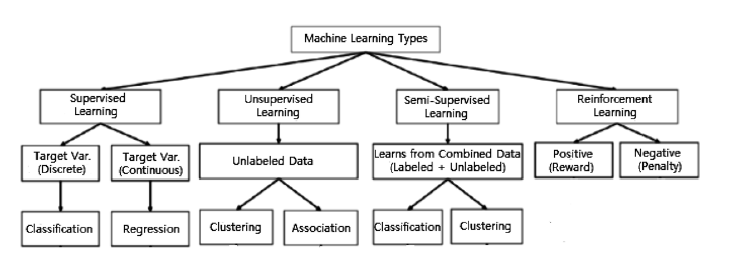
\includegraphics[width=1\textwidth]{imagens/TiposAprendizagens.png}
    \caption{Tipo de de Algoritmos de \textit{Machine Learning} \cite{10.1007/s42979-021-00592-x}.}
    \label{fig:tipoAprendizagem}
\end{figure}

Por outro lado, é importante de salientar que muitas vezes quando se fala em \textit{Machine Learning} apenas se referem ao procedimento de utilizar algoritmo de modelação para o problema em concreto, esquecendo-se de etapas essenciais de normalização e tratamento dos dados. Estas etapas são muito importantes, uma vez que a utilização de variáveis uniformizadas e escaladas é essencial para o melhor processo de treino dos algoritmos. Assim como a utilização de variáveis escaladas, é bastante importante a seleção das variáveis mais relevantes, isto é, aquelas que efetivamente têm importância na construção dos modelos, uma vez que permite diminuir a dimensionalidade e complexidade dos classificadores.


\subsection{\textit{Supervised Learning}}

A Aprendizagem Supervisionada é um dos tipos de algoritmo de \textit{Machine Learning}, sendo este um dos mais comuns e com mais casos de sucesso. Neste tipo de aprendizagem, o algoritmo é treinado de forma a que tente encontra uma relação entre as entradas e saída, ou seja entre as variáveis independentes e a variável dependente. Contudo não se pode aplicar este tipo de Aprendizagem em qualquer conjunto de dados, uma vez que é necessário que o conjunto de dados de saída este rotulado, seja este um rótulo categórico ou numérico \cite{inbook}. O modelo é criado a partir dos pares de variáveis independentes e dependentes, sendo posteriormente testado com um conjunto de dados nunca antes visto \cite{müller2016introduction}.    

Este tipo de Aprendizagem é amplamente utilizada em diversos tipos de problemas, tais como os problemas de Classificação, problemas de regressão, bem como de deteção de anomalias \cite{inbook}, sendo que nos problema de classificação o objetivo passa por fazer a previsão de um rótulo de uma lista pré-definida de possibilidades. Os problemas de classificação dividem-se ainda em problemas de classificação binária (divisão entre duas classes) e problemas de classificação multi-classe, onde a distinção ocorre entre mais de duas classes. Por outro lado, nos problemas de regressão, o objetivo passa por fazer a previsão de um número contínuo, que seja representado em termos matemáticos, tais como a previsão de idade de uma pessoa ou do seu salário anual \cite{müller2016introduction}.

\subsubsection{Generalização, \textit{Overfitting} e \textit{Underfitting}}

Tal como fora dito previamente, o objetivo de problemas de Aprendizagem supervisionada compreende a construção de modelos com o conjunto de dados de treino, sendo que posteriormente este modelo é testado num conjunto de dados de teste com as mesmas característica do conjunto de dados de treino, mas que não tenha sida visto antes \cite{müller2016introduction}. Neste processo, quando o conjunto de dados de teste apresenta previsões precisas, pode-se afirmar que existiu uma generalização para o conjunto de dados de teste a partir do conjunto de dados de treino, sendo que o objetivo passa por ter um modelo que faça esta Generalização com a maior precisão possível.

Esta medida da generalização apenas pode ser medida no conjunto de dados de teste, pois é neste conjunto que se visualiza o quão bem o modelo se adapta a novos dados, e para isto acontecer a melhor forma é através da elaboração de modelo simples (não demasiado simplista), dado que a criação de modelos complexos ou demasiado simplistas pode fazer com que os modelos caiam em fenómenos de \textit{overfitting} ou \textit{underfitting}, respetivamente.

O fenómeno de \textit{Overfitting} acontece quando o modelo apresenta resultados muito positivos no conjunto de dados de treino, contudo no conjunto de dados de treino estes resultados são inferiores. Este problema acontece quando o modelo se adapta demasiado ao conjunto de dados de treino, sendo este incapaz de fazer a previsão da mesma forma quando testado num conjunto de dados novo, ou seja, o modelo é muito específico para os dados de treino e não consegue realizar a generalização para os novos dados que possam surgir.

Por outro lado, também existe o problema de \textit{Underfitting}, que acontece quando o modelo é demasiado simples, não sendo capaz de fazer a captura de todos os aspetos e da variabilidade do conjunto de dados, onde o modelo se adapta mal, inclusive no conjunto de dados de treino. Desta forma, torna-se necessário encontrar o ponto perfeito intermediário entre estes dois possíveis fenómenos, que é onde se encontra a melhor performance ao nível de Generalização, tal como se pode visualizar na Figura \ref{fig:tradeoff}.


\begin{figure}[H]
    \centering
    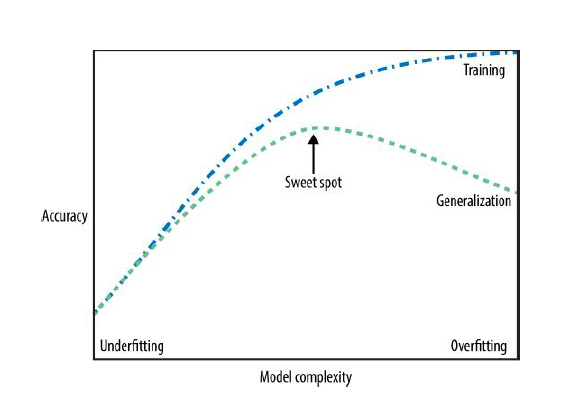
\includegraphics[width=0.9\textwidth]{imagens/tradeoffmodel.png}
    \caption{\textit{Trade-off} entre a Generalização do modelo, \textit{Overfitting} e \textit{Underfitting} \cite{müller2016introduction}.}
    \label{fig:tradeoff}
\end{figure}


\subsection{\textit{Unsupervised Learning}}

Ao contrário da Aprendizagem Supervisionada, a aprendizagem não Supervisionada não apresenta rótulos, ou seja, não apresenta uma variável dependente. Uma vez que estes dados não apresentam rótulo, ao contrário de de tentar fazer uma previsão ou uma classificação, neste tipo de aprendizagem visa-se encontrar estruturas ou padrões subjacentes aos dados, sendo o maior objetivo a descoberta de informações existentes nos próprios dados \cite{10.1007/s42979-021-00592-x}. Nesta aprendizagem, ao modelo apenas são apresentados os dados de \textit{input}, ao qual se espera que o modelo faça a extração de conhecimento, isto é, uma espécie de criação de rótulo ou categoria, de acordo com os dados provenientes.

Este tipo de Aprendizagem é amplamente utilizada em diversos tipos de problemas, sendo o \textit{Clustering} e o \gls{PCA} dois exemplos de algoritmos de Aprendizagem não-supervisionada \cite{10.1007/s42979-021-00592-x}, ou seja, em problemas de agrupamento de dados e problemas de transformação de dados. Um exemplo dos problemas de transformação de dados prende-se com redução da dimensão, em que existe um \textit{dataset} altamente dimensional, com bastantes \textit{features} como input. Nestes problemas, o \textit{output} é um \textit{dataset} muito mais conciso, representado por muito menos \textit{features} mas em que não se perca informação.

Na Figura \ref{fig:supuns} elabora-se uma representação da dualidade entre a Aprendizagem Supervisionada e a Aprendizagem não supervisionada, onde é possível a verificação da diferença ao nível da existência e não existência de rótulos nos dados, bem como uma diferenciação ao nível dos \textit{outputs} de ambos os algoritmos.

\begin{figure}[H]
    \centering
    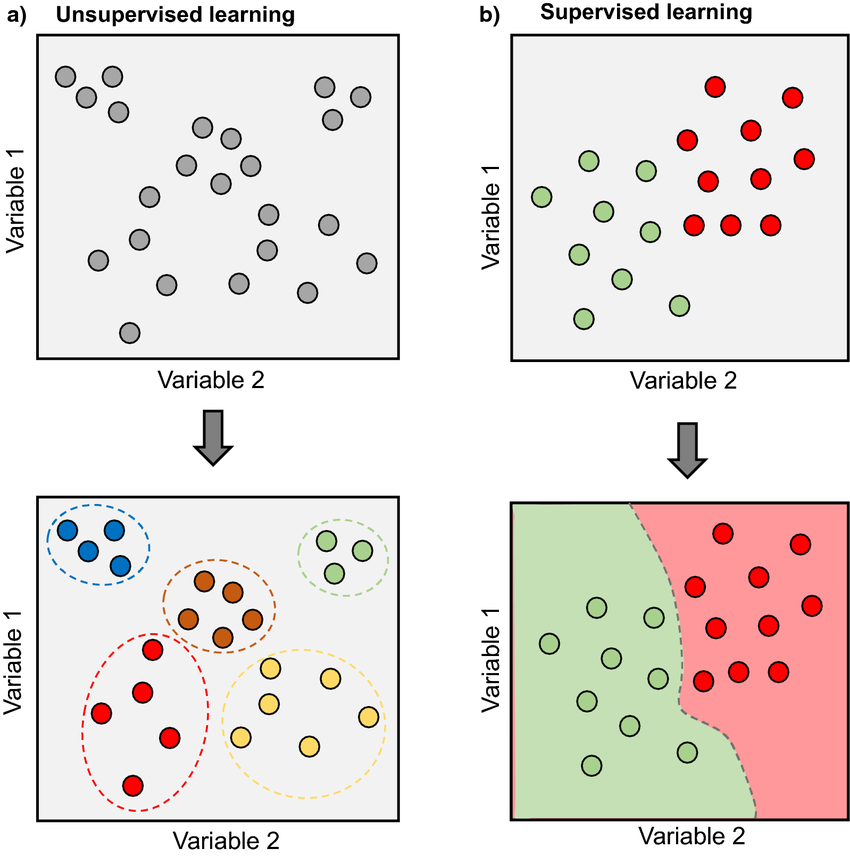
\includegraphics[width=0.7\textwidth]{imagens/Supervised-and-unsupervised-machine-learning-a-Schematic-representation-of-an.png}
    \caption{Diferenciação entre Aprendizagem Supervisionada e Aprendizagem Não Supervisionada \cite{unsupervisedimage}.}
    \label{fig:supuns}
\end{figure}

\subsection{\textit{Semi-Supervised Learning}}

A Aprendizagem Semi-Supervisionada, bem como o seu próprio nome indica, trata-se um paradigma de aprendizagem que combina elementos de Aprendizagem Supervisionada com elementos de Aprendizagem Não Supervisionada. Este tipo de Aprendizagem caracteriza-se pela utilização de um conjunto de dados misto, ou seja, uma mistura de exemplo com rótulos e dados sem rótulos, dados característicos de Aprendizagem Supervisionada e Não-Supervisionada, respetivamente \cite{10.1007/s42979-021-00592-x}.

\subsection{\textit{Reinforcement Learning}}

\textit{Reinforcement Learning}, ou Aprendizagem por Reforço, é um tipo de Aprendizagem diferentes dos Modelos de Aprendizagem Supervisionada ou Não Supervisionada, em que um agente aprende a tomar decisões e ações em conjunto com o ambiente que o rodeia, ou seja, o agente avalia automaticamente o comportamento  que deve ser com o contexto e ambiente em que se insere, sendo esta a principal diferença com o tipo de Aprendizagens previamente mencionadas, dado que a Aprendizagem por reforço tem por base a interação do agente com o ambiente, onde numa fase inicial não existem dados que ajudem na toma de decisões \cite{10.1007/s42979-021-00592-x}.

Neste tipo de Aprendizagem o Modelo aprende de forma autónomo, ou seja, a Aprendizagem é baseada em recompensas ou penalidades, onde o seu objetivo final é a maximização acumulativa da recompensa e a minimização do risco ao longo do tempo. Este tipo de algoritmo é muito importante em processos de automação e em sistema de robótica autónomos \cite{10.1007/s42979-021-00592-x}.

\subsection{Análise dos variados tipos de Aprendizagem de \textit{Machine Learning}}

\subsubsection*{Aprendizagem Supervisionada:}
Na Aprendizagem Supervisionada, os algoritmos são treinados usando um conjunto de dados que possui rótulos, ou seja, entradas acompanhadas de suas saídas desejadas. Essa abordagem é particularmente útil quando queremos realizar previsões ou classificações com base em exemplos históricos. É eficaz em situações em que desejamos fazer previsões usando dados previamente rotulados.

\textbf{Vantagens:}
\begin{itemize}
    \item Ideal para previsão e classificação com dados rotulados.
    \item Eficaz em cenários de previsões baseadas em dados históricos.
\end{itemize}

\textbf{Desvantagens:}
\begin{itemize}
    \item Dependência de dados rotulados.
    \item Limitado à qualidade e representatividade do conjunto de treinamento.
\end{itemize}

\subsubsection*{Aprendizagem Não Supervisionada:}
Na Aprendizagem Não Supervisionada, os algoritmos são treinados com dados que não possuem rótulos predefinidos. Sua utilidade está em descobrir padrões intrínsecos nos dados, sendo valiosa para a segmentação de dados, redução de dimensionalidade e detecção de anomalias. É comumente utilizada na análise exploratória de dados e geração de insights a partir de grandes conjuntos não estruturados.

\textbf{Vantagens:}
\begin{itemize}
    \item Descobre padrões em dados não rotulados.
    \item Útil para análise exploratória e geração de insights.
\end{itemize}

\textbf{Desvantagens:}
\begin{itemize}
    \item Requer análise mais aprofundada do conjunto de dados.
    \item Menos eficaz em tarefas que exigem conhecimento prévio dos dados.
\end{itemize}

\subsubsection*{Aprendizagem por Reforço:}
Na Aprendizagem por Reforço, os algoritmos aprendem a tomar decisões interagindo com um ambiente, recebendo recompensas ou penalizações com base em suas ações. Essa abordagem é adequada para otimizar processos sequenciais, como jogos, controle de robôs e tomada de decisões em tempo real, onde as ações impactam o ambiente e o agente precisa aprender com a experiência.

\textbf{Vantagens:}
\begin{itemize}
    \item Otimização de processos sequenciais.
    \item Adequada para ambientes interativos e tomada de decisões em tempo real.
\end{itemize}

\textbf{Desvantagens:}
\begin{itemize}
    \item Pode exigir um grande número de interações para aprender efetivamente.
    \item A complexidade do ambiente pode aumentar a dificuldade de aprendizado.
\end{itemize}
 
\section{Etapas de processo de \textit{Machine Learning}}

O processo de \textit{Machine Learning} envolve diversas etapas, que são geralmente organizadas em uma sequência lógica. As etapas a seguir descrevem o ciclo típico de desenvolvimento de um modelo de \textit{Machine Learning} utilizado no presente trabalho.

\subsection{Colheita, Compreensão e Identificação dos Dados}

A primeira etapa é a colheita  de dados relevantes para a área de Negócio envolvida no Problema, sendo que os dados podem ser obtidos de diversas fontes, tais como base de Dados, sensores, arquivos ou pedidos feitos via web. 

Uma vez adquiridos os dados, é necessário realizar a sua compreensão, bem como a sua identificação, através da descrição dos mesmos, exploração, bem como a verificação da sua qualidade.
\subsection{Preparação dos Dados}

Os conjuntos de dados nunca são perfeitos, e a maioria destes apresenta valores omissos, apresentam \textit{outliers}, bem como valores que não apresentem qualquer sentido para o contexto do negócio. Desta forma, os \textit{datasets} obtidos necessitam de serem lidos e formatados frequentemente, de forma a puderem ser utilizados para a obtenção de conhecimento.

Nesta etapa de Preparação ou pré-processamento dos dados utilizam-se como processos: remoção de valores ausentes ou substituição de valores ausentes, normalização ou estandardização dos dados, tratamento de \textit{outliers}, verificação de correlação entre atributos, de forma a promover a redução de atributos, e também muitas vezes a geração de novos atributos a partir dos dados já existentes.

\subsection{Divisão dos Dados}

Por norma, existe uma divisão dos dados antes da aplicação dos algoritmos. Desta forma, os dados normalmente se dividem em 2 ou 3 conjuntos, sendo treino e teste ou treino, validação e teste, respetivamente. Nesta prática, o conjunto de dados de treino é utilizado para o treinamento do modelo, o conjunto de dados de validação é utilizado para o ajuste de hiperparâmetros e avaliação do modelo, sendo que o conjunto de dados de teste é utilizado para a avaliação final do modelo. 

\subsection{Seleção do Algoritmo}

Nesta fase, tendo em conta o contexto do problema em estudo, bem como a organização dos conjuntos de dados em questão, procede-se com a seleção dos algoritmos adequados. Este processo não é um processo fácil, pois os Algoritmos tanto apresentam bons resultados para um problema, como apresentam resultados muito mais satisfatórias na previsão de outro problema.

\subsection{Treino do Algoritmo selecionado}

Nesta etapa, o modelo do Algoritmo é alimentado com o conjunto de Dados de treino, de forma a que possa estudar a relação entre as entradas e as saídas, ou seja, as respetivas classes. O modelo ajusta seus parâmetros para minimizar a diferença entre as previsões e a classe real.

\subsection{Avaliação do Algoritmo selecionado}

Uma vez terminada a fase de treino do algoritmo, torna-se necessária a Avaliação do Algoritmo selecionado. Esta fase utiliza o conjunto de dados de teste e avalia assim a precisão e \textit{accuracy} do modelo, tentando que se garanta a maior taxa de sucesso, evitando fenómenos de \textit{underfitting} ou \textit{overfitting}.

\subsection{Melhoria e ajuste de Parâmetros}

Após a fase de avaliação do Algoritmo, é necessário que se verificar se o algoritmo implementado pode ser melhorado, isto é, se este pode obter melhores métricas de avaliação. Tendo em conta este pressuposto, alteram-se os hiperparâmetros do modelo de forma a que sejam ajustados para a otimização máxima do desempenho do modelo. Uma vez alterado o conjunto dos hiperparâmetros, procede-se novamente ao treino e avaliação do Modelo.

\section{Técnicas de Preparação dos dados}

\subsubsection{Normalização}

A normalização, na área de \textit{Machine Learning} é uma das técnicas utilizadas na etapa de Pré-processamento dos dados, que tem por finalidade o ajuste da escala das \textit{features} numéricas, uma vez que diversas técnicas de \textit{Machine Learning} são sensíveis à escala dos dados, tendo assim impacto na performance dos modelos. Desta técnicas destacam-se algoritmos como a Regressão Linear, o \gls{NN} e o \gls{SVM}. Neste sentido, um atributo que apresente unidades mais pequenas terá uma menor importância, quando comparado com um atributo com unidades maiores, contudo isto será ultrapassado recorrendo a duas técnicas existentes de normalização de dados: \textit{Min-Max Scaling} ou \textit{Z-Score Normalization}.

A \textit{Min-Max Scaling} é uma técnica estatística que coloca os valores dos atributos num intervalo de valores específico, geralmente entre 0 e 1. Esta normalização assenta na seguinte equação:

\begin{align}
x_{\text{norm}} &= \frac{x - x_{\text{min}}}{x_{\text{max}} - x_{\text{min}}}\label{eq:minmax}
\end{align}

Por outro lado, \textit{Z-Score Normalization} é uma técnica de pré-processamento de dados que ajusta os valores dos atributos de forma a que estes tenham uma média de 0 e um desvio padrão de 1, tornando assim os atributos comparáveis e tornando a deteção de outliers mais fácil. Esta normalização assenta na seguinte equação:

\begin{align}
x_{\text{norm}} = \frac{x - \mu}{\sigma}\label{eq:zscore}
\end{align}

\subsubsection{Correlação de \textit{Pearson}}

De forma a avaliar a Independências entre as \textit{features} de \textit{input}, verificou-se a correlação entre as features através da utilização do coeficiente de Correlação de \textit{Pearson}, uma vez que permite reduzir a redundância.


A correlação de \textit{Pearson} trata-se de uma medida estatística que estuda a correlação linear existentes entre duas variáveis, sendo que os seus valores variam entre -1 e 1, que representam uma correlação negativa perfeita (quando uma variável aumenta a outra variável diminui) e uma correlação positiva perfeita (quando uma variável aumenta a outra variável também aumenta), respetivamente. No que diz respeito ao valor, o valor de 0 representa a ausência de relação linear entre as variáveis, onde não existe nenhum tendência entre as duas variáveis \cite{Akoglu2018}. A existência de Correlação positiva, correlação negativa e ausência de correlação encontra-se apresentada na Figura \ref{fig:pearson}, respetivamente.

\begin{figure}[H]
    \centering
    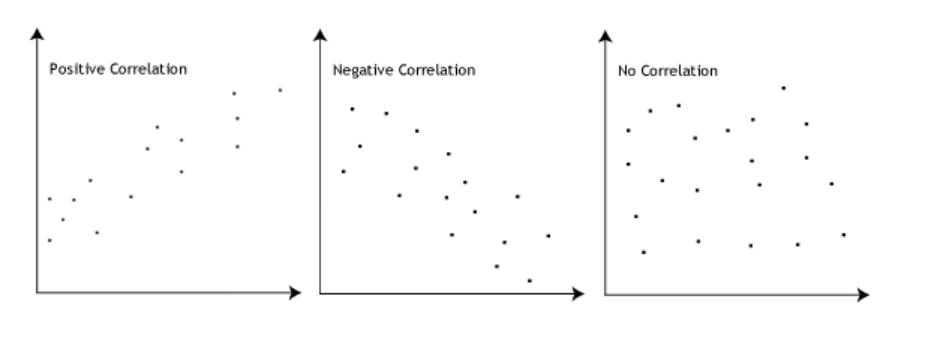
\includegraphics[width=1\textwidth]{imagens/pearsoncorrelation.png}
    \caption{Correlação de \textit{Pearson} \cite{pearson_website}.}
    \label{fig:pearson}
\end{figure}


\subsubsection{VIF}

É importante a análise de Correlação entre atributos, de forma a promover a redução do número de atributos como \emph{Input} dos Algoritmos de  \emph{Machine Learning}, bem como a promoção de redução de fenómenos de \emph{Overfitting}. 

Para análise de correlação entre os diferentes atributos, optou-se pela utilização do fator \gls{VIF}.

Este Algoritmo, é um indicador de multicolinearidade usado para a avaliação de correlação entre os diferentes atributos, onde multicolinearidade ocorre quando uma ou mais variáveis independentes têm uma forte correlação entre si. 

O valor de fator \emph{VIF} divide-se em 3 possíveis acontecimentos:
\begin{itemize} 
\itemsep-0.5em 
    \item Se \emph{VIF} é igual a 1, não existe correlação;
    \item Se  \emph{VIF} é maior que 1 e menor que 5, existe correlação intermédia; 
    \item Se \emph{VIF} é maior que 10, existe alta correlação;
\end{itemize}

\subsubsection{\gls{PCA}}

Atualmente, muitos dos conjuntos de dados existente apresentam quantidade de dados enormes, com um número considerado de \textit{features}, em que dificulta a análise do mesmo, sendo muitas destas \textit{features} redundantes, apresentando muitas das vezes informação duplicada. De forma a ser possível uma boa análise a estes conjuntos, torna-se necessário reduziar a sua dimensionalidade, aplicando algoritmo de seleção de \textit{Features}, tal como o \gls{PCA}.

O \gls{PCA} é uma técnica de aprendizagem não supervisionada consideravelmente utilizada para o propósito de seleção de \textit{Features}, reduzindo a dimensionalidade mas tem perca de informação pertinente.


\subsubsection{Balanceamento de \textit{Datasets}}

Muitos dos conjuntos de dados existentes encontram-se desbalanceados, representados por uma classe maioritária e uma ou mais classes minoritárias. No que diz respeito ao desbalanceamento em dados relativos à saúde, a classe maioritária usualmente é a ausência de uma doença.

Posto isto, é necessária a existência de um processo que permita o balanceamento dos conjuntos de dados, acabando assim com a existência de dados desequilibrados e que permita uma distribuição homogénea por classe. Este equilíbrio é importante, uma vez que os Modelos de \textit{Machine Learning} apresenta dificuldades em aprender a classe com menos representações. Este tipo de problema tem bastante impacto em problemas de classificação. Usualmente, existem duas possíveis formas de combater o problema de desbalanceamento dos Conjuntos de dados:

\begin{itemize} 
\itemsep-0.5em 
    \item {\textbf{Oversampling (Supersampling)}}: Criação de cópias adicionais de dados da classe minoritária até que o equilíbrio entre as classes seja alcançado.
    \item {\textbf{Undersampling (Subsampling)}}: Redução do número de dados da classe maioritária até que o equilíbrio entre as classes seja alcançado. A redução dos dados pode ser feita de forma aleatória ou através da utilização de determinados critérios. 
\end{itemize}

Contudo, esta duas técnicas também apresentam desvantagem, sendo que o \textit{Oversampling} aumenta o risco de \textit{overfitting}, ao mesmo tempo que aumenta o tempo de treino dos algoritmos. Por outro lado, o \textit{Undersampling} pode levar à diminuição da qualidade, uma vez que se podem retirar informações pertinentes da classe maioritária, apesar de aumentar a rapidez do algoritmo. Posto isto, atualmente existem algoritmos mais avançados que permitem este equilíbrio, tal como o \gls{SMOTE}, que faz a criação sintética de dados da classe minoritária, contudo não replicados dados existentes, o que reduz a probabilidade de \textit{overfitting}.

A técnica de \gls{SMOTE}, como se trata de uma técnica de geração de dados, é uma técnica de \textit{Oversampling}, contudo esta criação é baseada nas semelhança entre os dados da classe minoritária.



\subsubsection{\textit{Cross-Validation}}

Relembrando que o objetivo da divisão do conjunto de dados total, em conjunto de dados de treino e conjunto de dados de teste, e que o pretendido é que o modelo se adapte corretamente  a novos dados, surge o processo de \textit{Cross-Validation}.

O \textit{Cross-Validation} é um método estatístico de avaliação e de comparação de algoritmos de \textit{Machine Learning}, que é mais estável do que uma simples divisão em Conjunto de dados de treino e de teste, uma vez que permite caracterizar se o modelo é capaz de generalizar bem para diferentes conjuntos de dados. Enquanto a simples divisão em conjunto de dados de treino e de teste é feita de forma aleatória, enquanto que no \textit{Cross-Validation}, cada exemplo vai estar no conjunto de dados de treino e de teste uma vez, assegurando a generalização. Ao nível de desvantagens do uso de \textit{Cross-Validation}, destaca-se o aumento do custo computacional, uma vez que faz o treino de k modelos e não o treino de apenas 1 modelo.

Neste processo, o conjunto de dados é dividido continuamente e são utilizados diversos modelos. A forma mais comum de utilização de \textit{Cross-Validation} é denominada de \textit{K-fold Cross-validation}, onde k é um número especificamente, usualmente 5 ou 10, que representa o número de divisões. Por exemplo, quando se utiliza o processo de \textit{5-fold Cross-Validation}, o conjunto de dados é dividido em 5 sub-conjuntos de tamanho igual. Uma vez realizada esta divisão, são procedidos ao treino e testa, sendo o primeiro \textit{fold} utilizado como conjunto de teste e os restantes como conjunto de treino, ou seja, o modelo é construído com os \textit{folds} 2-5 e depois é avaliado recorrendo ao primeiro \textit{fold}. Posteriormente, utiliza-se o segundo \textit{fold} como conjunto de dados de testes, e o restantes \textit{folds} como conjunto de dados de treino. O processo é repetido iterativamente com os seguintes \textit{folds} como junto de teste. Por último, extrai-se o valor da \textit{accuracy} para cada um das divisões em conjunto de dados de treino e de teste \cite{müller2016introduction}. Este processo encontra-se ilustrado na Figura \ref{fig:cross}.

\begin{figure}[H]
    \centering
    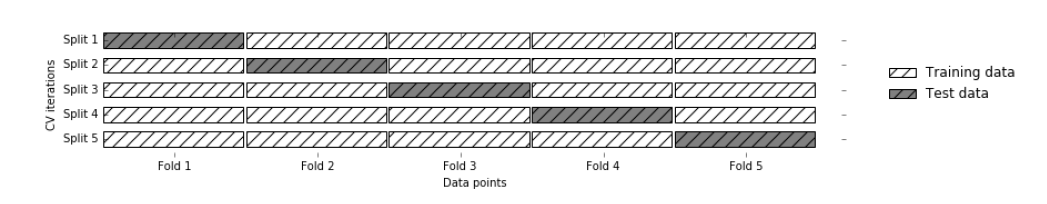
\includegraphics[width=1\textwidth]{imagens/cross-validation.png}
    \caption{Explicação do Processo de \textit{Cross-Validation} \cite{müller2016introduction}.}
    \label{fig:cross}
\end{figure}

Em problemas de classificação, a biblioteca de Scikit-learn, quando utiliza \textit{Cross-Validation}, faz por meio de \textit{Stratified k-fold cross-validation}, onde se assegura que são mantidas proporções semelhantes entre os elementos de cada uma das classes em cada um dos \textit{folds}. Este processo encontra-se ilustrado na Figura \ref{fig:stratifiedcross}.

\begin{figure}[H]
    \centering
    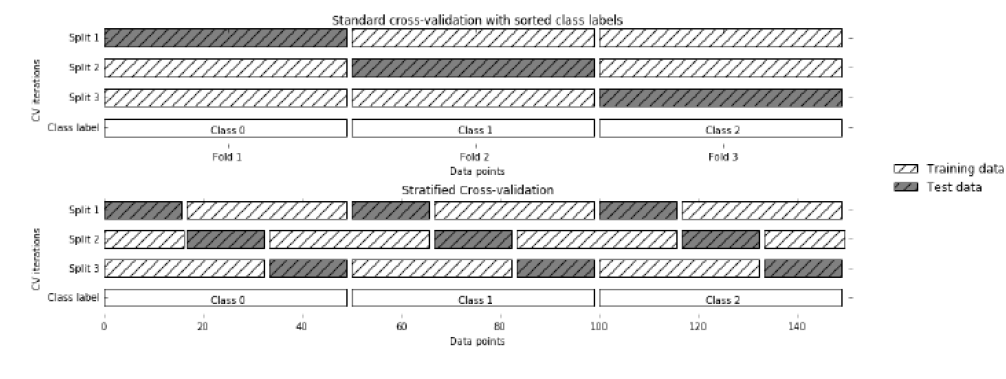
\includegraphics[width=1\textwidth]{imagens/stratifiedcrossvalidation.png}
    \caption{Explicação do Processo de \textit{Stratified k-fold Cross-Validation} \cite{müller2016introduction}.}
    \label{fig:stratifiedcross}
\end{figure}


\subsubsection{\textit{Tuning} de Hiperparâmetros}

O processo de \textit{Tuning} de Hiperparâmetros, ou seja, a otimização dos parâmetros de um Modelo de \textit{Machine Learning} não é uma tarefa que seja facilmente realizada de forma manual, contudo apresenta resultados significativos no desempenho do modelo nos dados de validação e de teste. Estes parâmetros controlam aspetos importantes dos modelos, sendo que diferentes modelos apresentam diferentes parâmetros, e caso estes parâmetros não sejam escolhidos corretamente pode-se cair em fenómenos de \textit{Overfitting} ou \textit{Underfitting}.

Dado a complexidade dos modelos, e a dificuldade em se conseguir obter o valor dos parâmetros ótimos de forma manual, existem métodos computacionais capazes de fazer este processo e em tempo mais reduzido. Como esta tarefa é bastante comum, já existem métodos standard no biblioteca de \textit{Scikit-learn} que a permitem. O método mais utilizado é o \textit{GridSearch}, em que de forma resumida se tenta todas as possibilidade do conjunto de parâmetros de interesse.

\subsubsection{Seleção de \textit{features}}

A Etapa de Seleção de \textit{features} apresenta bastante impacto na elaboração e na performance de Modelos preditivos de \gls{ML}, nomeadamente no ponto de vista de precisão, como do ponto de vista temporal. Revela-se uma etapa bastante importante, nomeadamente, em conjuntos de dados que apresentem elevada dimensionalidade, ou seja, em conjunto de dados em que a quantidade de features é bastante elevada, aumentando assim a complexidade do modelo. Posto isto, torna-se necessária esta etapa, nomeadamente devido aos seus benefícios:
\begin{itemize}
    \item Redução da Complexidade do problema.
    \item Aumento da Performance do modelo.
    \item Diminuição do risco de fenómenos de \textit{Overfitting}, através da diminuição de \textit{features} redundantes.
    \item Diminuição do tempo de treino do algoritmo.
\end{itemize}

Apesar desta etapa estar diretamente ligada com a eficácia dos Modelos, esta etapa é demasiadas vezes ignorada, devido à ausência de conhecimento acerca de métodos de seleção de \textit{features}, ou ao baixo tempo necessário para a implementação de projetos. Tendo em conta estes pressupostos, o objetivo nesta etapa passa pela implementação de métodos de seleção de \textit{features} robustos, reutilizáveis e praticamente automatizados, dos quais são exemplo os seguintes métodos:
\begin{itemize}
    \item Análise de \textit{features} categóricas e correlação entre \textit{features}.
    \item Importância das features através de Modelos como o \gls{RF} e o \Gls{XGBoost}.
    \item Coeficientes de Lasso.
    \item \gls{RFE}
\end{itemize}

De um ponto de vista visual, esta etapa ao longo de uma Pipeline de projetos de \gls{ML}, representa a etapa em que existe a diminuição de quantidade de \textit{features} existente, sem existir redução de quantidade de informação pertinente, ou seja, não afetando a precisão do modelo, apenas retirando as \textit{features} redundantes, tal como se visualiza na Figura \ref{fig:featureSelection}, onde a quantidade de \textit{features} é reduzida, devido à redundância entre as mesmas.

\begin{figure}[H]
    \centering
    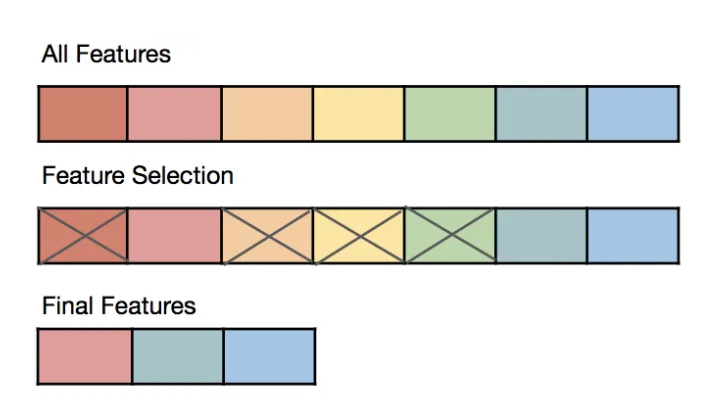
\includegraphics[width=1\textwidth]{imagens/FeatureSelection.png}
    \caption{Redução do Número de \textit{Features} \cite{automated-feature-selection}.}
    \label{fig:featureSelection}
\end{figure}

\section{Algoritmos de Aprendizagem Supervisionada}

\subsection{\textit{Linear Regression} e \textit{Logistic Regression}}

O algoritmo mais simples de Aprendizagem Supervisionada é a Regressão Linear, que representa uma reta com uma variável independente (x) e uma variável dependente (y), sendo que o objetivo desta reta é a obtenção do menor erro possível na previsão do valor da variável dependente (y = mx + b).

Num ponto de vista mais realista dos problemas existentes, esta regressão transforma-se numa Regressão multivariada, onde existem várias variáveis independentes (y = m1x1 + m2x2 + m3x3 + ... + mnxn), onde n representa o número de atributos, sendo que o objetivo é a descoberta dos melhores valores para m, de forma a reduzir a soma dos quadrados dos erros).

A Regressão Logística é uma técnica de \textit{Machine Learning} recomendada para situações em que a variável dependente é binária, ou seja, em problema de Aprendizagem Supervisionada de Classificação Binária, ou seja em problemas de resposta binária.

Nos problemas de Regressão Logística, estima-se a probabilidade de ocorrência de uma evento com base nas variáveis independentes do conjunto de dados. Como o resultado é uma probabilidade, a variável dependente encontra-se limitada entre 0 e 1, posto isto deve-se definir um \textit{threshold} para diferenciar entre classes, por exemplo se for superior a 50\% o algoritmo pertence à classe 1, enquanto se for inferior a 50\% representa a classe 0. A probabilidade é calculada de acordo com um função logística, onde o \textit{output} está entre 0 e 1, representada pela seguinte equação.


\begin{equation}
P(Y=1|X) = \frac{1}{1 + e^{-(\beta_0 + \beta_1X_1 + \beta_2X_2 + \ldots + \beta_nX_n)}}
\end{equation}

A equação previamente referida representa a probabilidade de um determinado evento acontecer, dividido pela probabilidade de não ocorrência do mesmo evento, através de uma função sigmoide. A nível de problemas de classificação utiliza-se a Regressão Logística, uma vez que na Regressão Linear univariada existem valores superiores a 1 e valores inferiores a 0, o que não é o pretendido. De forma a distinguir os objetivos de ambas as regressões, verifica-se esta dualidade na representação da Figura \ref{fig:linearvslogist}.

\begin{figure}[H]
    \centering
    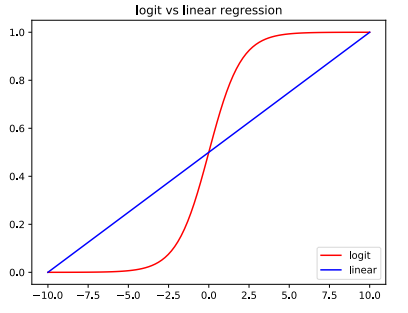
\includegraphics[width=0.6\textwidth]{imagens/linearvslogistic.png}
    \caption{Representação visual do Algoritmo de Regressão Linear e Regressão Logística.}
    \label{fig:linearvslogist}
\end{figure}


\subsection{\gls{NB}}

\textit{Naive Bayes} é um algoritmo baseado no Teorema de \textit{Bayes}. Este teorema descreve a probabilidade de um evento acontecer, com base no conhecimento prévio de condições que podem estar relacionadas para esse evento. O termo \textit{naive} (ingénuo) deve-se ao fato de o algoritmo não ter como base de partida uma certeza inicial, a partir do qual se constrói esse grau analisando as frequências presentes nos dados que temos disponíveis. Este algoritmo assenta na seguinte equação:

\begin{equation}
P(C_k | X) = \frac{P(C_k) \cdot P(X | C_k)}{P(X)}
\end{equation}

Onde:
\begin{align*}
& P(C_k | X) \text{ é a posterior probabilidade da classe } C_k \text{dadas as \textit{features} de entrada} X. \\
& P(C_k) \text{ é a probabilidade da classe } C_k. \\
& P(X | C_k) \text{ é a probabilidade de ter certas \textit{features} } X \text{ sabendo a classe } C_k. \\
& P(X) \text{ é a probabilidade de ter certas \textit{features} de entrada.}
\end{align*}


\subsection{\gls{DT}}

\textit{Decision Tree} é um algoritmo de Aprendizagem Supervisionada que tanto pode ser utilizado em problemas de regressão, como em problemas de Classificação. Neste algoritmo as árvores de decisão são geradas tendo por base o conjunto de dados de treino, sendo que resulta numa estrutura em forma de árvore para classificar os novos dados.

Cada árvore é composta por múltiplos níveis de \textit{nodes} que representam as \textit{features} do conjunto de dados e por \textit{branches}, que contém os possíveis valores que cada nó pode ter, sendo estes \textit{nodes}: \textit{Root node}, \textit{Decision nodes} (\textit{internal nodes}) e \textit{Leaf nodes} (\textit{Terminal nodes}).  

Para cada novo caso, o processo começa a partir do \textit{root node} e utilizando os valores de cada \textit{feature}, a árvore é percorrida até chegar ao \textit{leaf node}, onde é realizada a sua classificação. A figura \ref{fig:decisiontree} apresenta a representação visual de uma árvore de decisão \cite{Uddin2019ComparingDS}.

\begin{figure}[H]
    \centering
    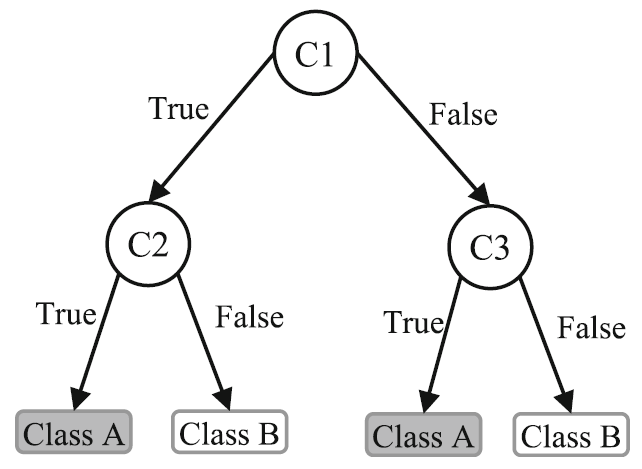
\includegraphics[width=0.6\textwidth]{imagens/decisiontree.png}
    \caption{Representação visual do Algoritmo de \gls{DT} \cite{Uddin2019ComparingDS}.}
    \label{fig:decisiontree}
\end{figure}

Este tipo de Algoritmo pode ser utilizado com diversos intuitos, contudo para demonstração do seu potencial, tendo em conta a área da saúde, escolheu-se a classificação do Risco de Prevenção de um ataque cardíaco, representado na Figura \ref{fig:heart}.

\begin{figure}[H]
    \centering
    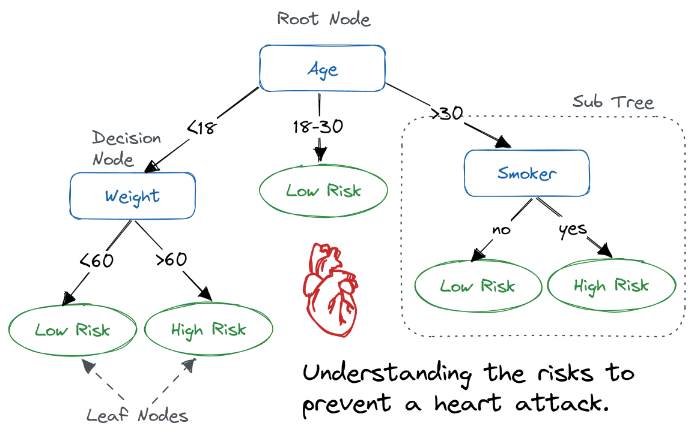
\includegraphics[width=0.8\textwidth]{imagens/decisionTreeRealExample.png}
    \caption{Representação visual do Algoritmo de \gls{DT} aplicado na vertente da saúde \cite{datacamp_decision_tree_tutorial}.}
    \label{fig:heart}
\end{figure}

Pela análise da árvore de decisão na Figura \ref{fig:heart}, verifica-se o \textit{root node} e os \textit{Decision Nodes} são as característica da pessoa, tais como a Idade, peso e se é fumadora, sendo que o \textit{leaf node} é o resultado final, ou seja, o baixo ou alto risco de previsão de um ataque cardíaco  \cite{datacamp_decision_tree_tutorial}. 


\subsection{\gls{RF}}

O Algoritmo \textit{Random Forest} é um algoritmo de Aprendizagem Supervisionada, principalmente utilizado em problemas de classificação e regressão. Trata-se de um algoritmo que combina o resultado de várias árvores de decisão, resultando numa floresta aleatória, em que se calcula a média/moda dos resultados das árvores de decisão (dependendo se o \textit{output} é numérico ou categórico), permitindo assim uma melhoria de precisão e redução de fenómenos de \textit{overfitting}. Nesta floresta aleatória, cada uma das árvores de decisão, possui a sua própria estrutura interna, contudo com o mesmo tipo de resultado final. A utilização deste algoritmo é diretamente proporcional com a quantidade de árvores de decisão.

Um exemplo de como este algoritmo funciona, pode ser visualizado na Figura \ref{fig:randomforest}.

\begin{figure}[H]
    \centering
    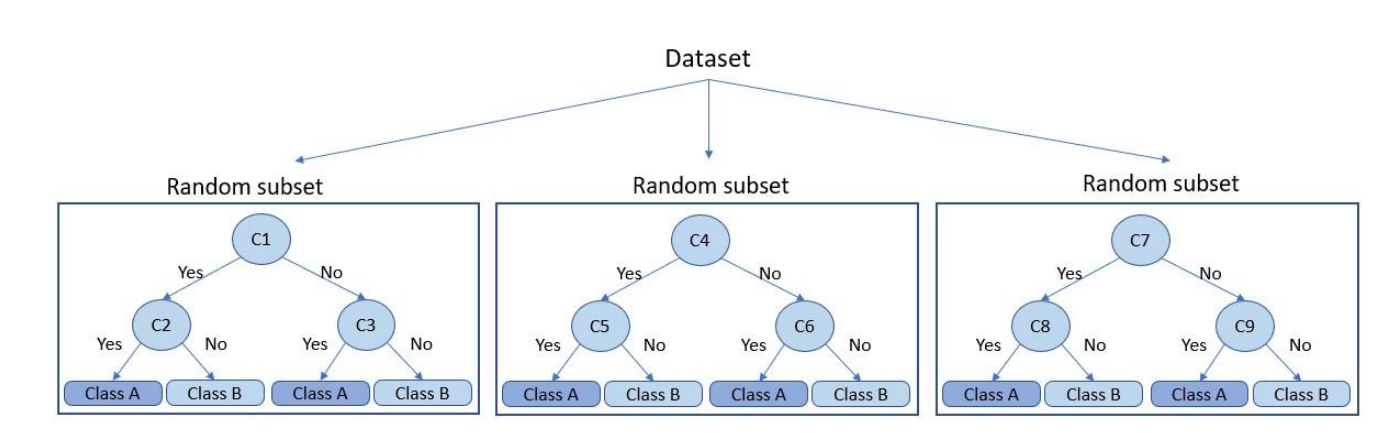
\includegraphics[width=0.9\textwidth]{imagens/randomforest.png}
    \caption{Representação visual do Algoritmo de \gls{RF} \cite{Uddin2019ComparingDS}.}
    \label{fig:randomforest}
\end{figure}


\subsection{\textit{K-Nearest Neighbors}}

O \textit{K-nearest neighbour} é um dos algoritmos mais simplista utilizados em problemas de regressão e classificação em Aprendizagem Supervisionada. Este algoritmo é baseado no princípio de proximidade, onde objetos semelhantes devem estar próximo de outros semelhantes. O K presente no nome do algoritmo representa o número de vizinhos próximos que são considerados no problema de classificação, onde a utilização de diferentes números de k, origina diferentes resultados no processo de classificação, tal como se verifica na Figura \ref{fig:knn}, onde por exemplo para k = 3, o nome objeto é classificado como preto, enquanto que no k = 5, o objeto é classificado como vermelho \cite{Uddin2019ComparingDS}.

\begin{figure}[H]
    \centering
    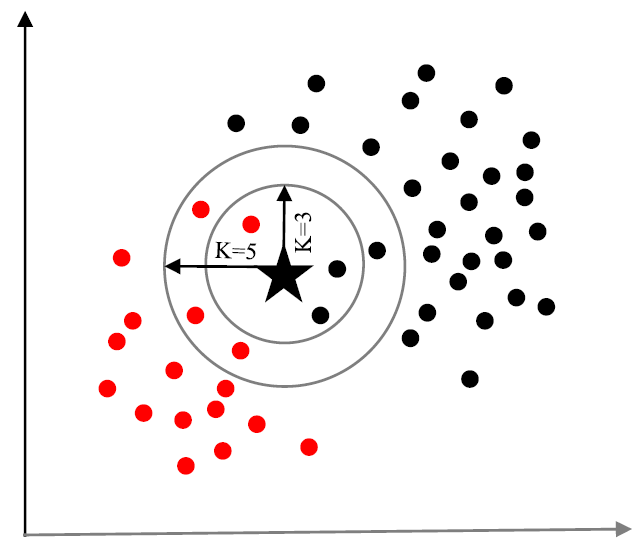
\includegraphics[width=0.6\textwidth]{imagens/KNN.png}
    \caption{Representação visual do Algoritmo de \gls{NN} \cite{Uddin2019ComparingDS}.}
    \label{fig:knn}
\end{figure}


\subsection{\gls{SVM}}

O \gls{SVM} é um algoritmo que tanto permite realizar a classificação de dados linear, como de dados não lineares e tanto pode ser utilização em classificação binária como em classificação multi-classe. Este algoritmo começa pela realização de uma mapeamento do conjunto de dados para um espaço de n dimensões, onde n é o número de \textit{features} no conjunto de dados. Posteriormente, o \gls{SVM} representa estes ponto num espaço bidimensional, e tentar encontrar um hiperplano ideal, que separe os dados em duas classes enquanto maximiza a distância marginal (distância entre o hiperplano de decisão e a instância que representa a classe) entre as duas classes, diminuindo assim os erro de classificação. Na Figura \ref{fig:svm} pode-se verificar um exemplo visual do algoritmo de \gls{SVM} \cite{Uddin2019ComparingDS}.

\begin{figure}[H]
    \centering
    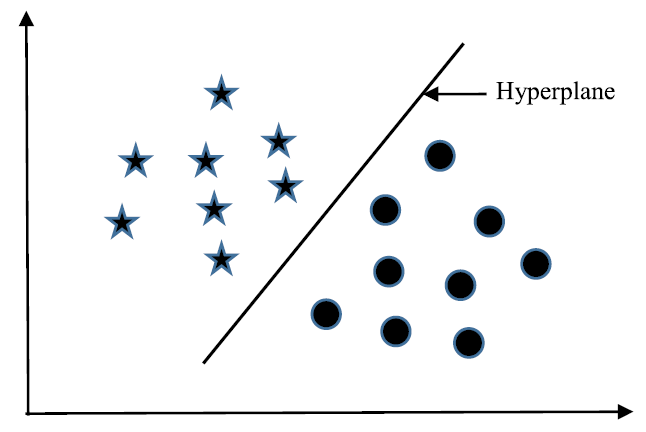
\includegraphics[width=0.6\textwidth]{imagens/svm.png}
    \caption{Representação visual do Algoritmo \gls{SVM} \cite{Uddin2019ComparingDS}.}
    \label{fig:svm}
\end{figure}


\subsection{\textit{Ensemble}}

\textit{Ensemble Learning} é uma técnica de \textit{Machine Learning} em que existe a combinação de múltiplos modelos de forma a melhorar a performance de modelos de aprendizagem supervisionada de Previsão ou de Classificação, ou mesmo reduzir a probabilidade de realizar uma previsão ou classificação errada. Neste contexto, esta técnica em vez de depender de apenas um modelo, utilizar diversos modelos para conseguir melhorar o algoritmo, tornando este mais preciso \cite{thanoun}. 

\subsubsection{\textit{XGBoost}}

\gls{XGBoost} é um algoritmo de Machine Learning baseado em árvores de decisão, bastante popular em problemas de Aprendizagem Supervisionada, tais como problemas de Regressão e de Classificação. Trata-se de uma algoritmo com a técnica de \textit{Gradient Boosting}, onde os modelos são construídos de forma sequencial, e são constantemente melhorados.


Além disto, o \gls{XGBoost} é um excelente algoritmo, uma vez que evita o fenómenos de \textit{Overfitting} devido ás suas técnicas de regularização.

\subsubsection{Técnica de \textit{Voting}}

O \textit{Voting Ensemble} é um método de \textit{Ensemble Learning}, que funciona de forma parecido com um sistema eleitoral, onde vários modelos de Machine Learning são treinados de forma individual, mas as suas previsões são combinadas através de votação \cite{thanoun}. Neste sentido, neste tipo de \textit{Ensemble}, diferenciam-se dois tipos de votação: \textit{Soft} e \textit{Hard Voting}. 
\begin{itemize}
    \item \textit{Hard Voting}:  O \textit{Hard Voting} é aplicado nas classes das previsões de cada modelo, em que as previsões de cada modelo são consideradas como votos e a classe que recebe mais de metade dos votos é selecionada como a classe da previsão final.
    \item \textit{Soft Voting}: Cada modelo fornece uma estimativa de probabilidade para cada classe e a média dessas probabilidades é calculada para determinar a previsão final.
\end{itemize}


\subsubsection{Técnica de \textit{Stacking}}

O \textit{Stacking}  é uma técnica de \textit{Ensemble Learning} onde as previsões de diversos modelos de Machine Learning são adicionadas a um conjunto de dados. O primeiro passo neste tipo de Técnica é a definição dos Modelos de \textit{Machine Learning} utilizados como Modelos Base, ou seja, os  modelos dos quais as previsões servem para a criação do conjunto de dados que será o input do Modelo Meta. Uma vez definidos estes modelos, faz-se o seu treino recorrendo ao conjunto de dados de treino, sendo que posteriormente realizam-se as previsões recorrendo ao conjunto de dados de teste, sendo estas previsões as \textit{features} de \textit{input} para o modelo Meta. Por fim, o Modelo Meta é treinado com recurso ao conjunto de dados com as previsões dos modelos Base e testado. Neste sentido, o objetivo deste tipo de técnica é melhorar o desempenho, de forma a que este seja superior ao que aos resultados dos modelos de forma individual \cite{thanoun}.


\section{Métricas de Avaliação}

Uma vez pensado o \textit{workflow} até ao processo de utilização do conjunto de dados de teste, segue-se a etapa de medição do desempenho do modelo, verificando-se se este efetua uma boa generalização do problema, ou seja, a qualidade das previsões obtidas. Posto isto, apresentam-se as principais métricas utilizadas em problemas de classificação, bem como as respetivas fórmulas.

Nos modelos de classificação, mais concretamente de Classificação binária (entre duas classes), o objetiva é a previsão de acordo com as duas classes possíveis, geralmente em casos de positivo ou negativo, presença ou ausência de um determinado evento. No âmbito da saúde, um exemplo é a presença ou ausência de uma determinada doença, possivelmente a doença de \textit{Parkinson}. Esta avaliação em problemas de classificação é realiza através da comparação entre a classe real e a classe obtida através dos modelos de previsão.

\subsection{Matriz de Confusão}

A qualidade de um modelo de classificação pode ser visualizada através de uma Matriz de Confusão, matriz esta que apresenta os seguinte tipos de dados:   

\begin{itemize} 
\itemsep-0.5em 
    \item \gls{VP}: Número de exemplo da classe positiva classificados corretamente.
    \item \gls{FP}: Número de exemplo da classe negativa classificados como sendo da classe positiva. 
    \item \gls{VN}: Número de exemplo da classe positiva classificados corretamente.
    \item \gls{FN}: Número de exemplo da classe positiva classificados como sendo da classe negativa.
\end{itemize}

Uma Matriz de Confusão de Classificação Binária é um \textit{array} de 2 por 2, onde as linhas representam as classes reais, enquanto que as colunas representas as classes previstas, onde cada entrada apresenta uma frequência de amostra, tal como se verifica na Figura \ref{fig:matrizbina}. Esta visualização é relevante, uma vez que de forma facilita se consegue visualizar quantos casos foram classificados de forma errada em cada uma das classes.

\begin{figure}[H]
    \centering
    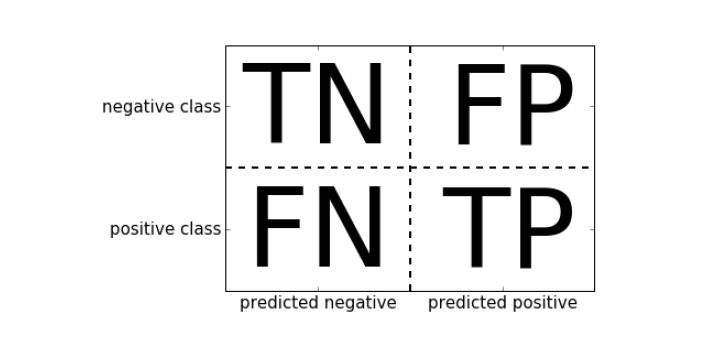
\includegraphics[width=1\textwidth]{imagens/matrizbina.png}
    \caption{Matriz de Classificação Binária \cite{müller2016introduction}.}
    \label{fig:matrizbina}
\end{figure}

Outro fator bastante importante da Matriz de Confusão, é que através desta representação e dos valores dos dados VP, FP, VN e FN, se conseguem calcular outras métricas de avaliação:  Taxa de Falso Positivo (Percentagem de acerto na classe negativa), Taxa de Verdadeiro Positivo (Percentagem de acerto na classe positiva), \textit{accuracy}, \textit{precision}, \textit{recall}, \textit{F1-Score}, sensibilidade (erro do tipo 2) e especificidade (erro do tipo 1).

\subsection{Sensibilidade}

A Sensibilidade corresponde à taxa de acerto na classe positiva. No contexto do problema, representa a possibilidade de previsão da doença de \textit{Parkinson}, e é calculada pela seguinte fórmula.

\begin{equation}
\text{Sensibilidade} = \frac{\text{Verdadeiros Positivos}}{\text{Verdadeiros Positivos} + \text{Falsos Negativos}}
\end{equation}

\subsection{Especificidade}

A Especificidade corresponde à taxa de acerto na classe negativa. No contexto do problema, representa a possibilidade de previsão da não existência da doença de \textit{Parkinson}, e é calculada pela seguinte fórmula.

\begin{equation}
\text{Sensibilidade} = \frac{\text{Verdadeiros Negativos}}{\text{Verdadeiros Negativos} + \text{Falsos Positivos}}
\end{equation}

\subsection{Accuracy}

A \textit{Accuracy} é calculada pela seguinte fórmula.

\begin{equation}
\text{Accuracy} = \frac{\text{Verdadeiros Positivos} + \text{Verdadeiros Negativos}}{\text{Total de Amostras}}
\end{equation}

\subsection{Precisão}

A precisão é a proporção de Verdadeiros Positivos em relação ao número
total de previsões positivas feitas pelo modelo. A \textit{Precisão} é calculada pela seguinte fórmula.

\begin{equation}
\text{Precisão} = \frac{\text{Verdadeiros Positivos}}{\text{Verdadeiros Positivos} + \text{Falsos Positivos}}
\end{equation}

\subsection{\textit{Recall}}

O \textit{Recall} é a proporção de verdadeiros positivos em relação
ao número total de exemplos positivos, sendo que é calculado pela seguinte fórmula.

\begin{equation}
\text{Precisão} = \frac{\text{Verdadeiros Positivos}}{\text{Verdadeiros Positivos} + \text{Falsos Negativos}}
\end{equation}

\subsection{\textit{F1-Score}}

O \textit{F1-Score}, uma média harmónica, que varia entre 0 e 1, calculada com base na precisão e no \textit{recall}. Esta métrica pode ser obtida com base na equação, é calculada pela seguinte fórmula.


\begin{equation}
\text{F1-Score} = 2 \cdot \frac{\text{Precisão} \cdot \text{Sensibilidade}}{\text{Precisão} + \text{Sensibilidade}}
\end{equation}

\subsection{\gls{ROC}}

A curva \gls{ROC} é um gráfico que permite proceder com a avaliação de um classificador binário, sendo este uma das métricas mais utilizadas para esta avaliação. 

Essa visualização leva em consideração a taxa de verdadeiros positivos e a taxa de falsos positivos, onde no eixo dos X está representada a Especificidade, enquanto que no eixo dos Y está representa a Sensibilidade. Neste gráfico podem-se representar diversos classificadores e verificar qual deles apresenta melhores resultados, sendo que quanto mais próximo o classificador estiver do topo do eixo dos Y melhor será o classificador. O desempenho total é gerado pela \gls{AUC}, que representa a área de forma dimensional debaixo da curva, onde um valor de aproximadamente 0,5 representa um classificador aleatório, enquanto que um valor de aproximadamente 1 representa um classificador ideal, que é capaz de diferenciar duas classes, tal como se pode verificar na Figura \ref{fig:roc}.


\begin{figure}[H]
    \centering
    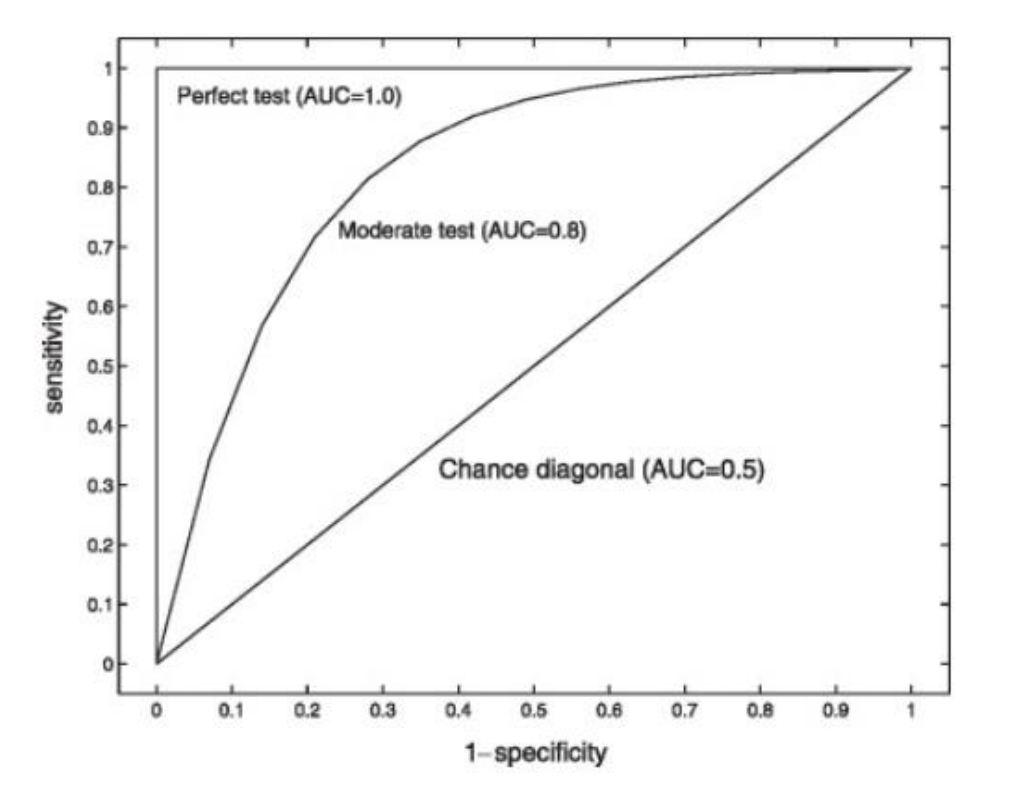
\includegraphics[width=0.7\textwidth]{imagens/roc.png}
    \caption{Representação gráfica da curva \gls{ROC}.}
    \label{fig:roc}
\end{figure}

\chapter{O Caso de estudo}
\section{Levantamento dos Dados}

O \textit{Dataset} utilizado foi obtido num repositório da Universidade de Califórnia \textit{Irvine} “\textit{UCI Machine Learning Repository}”, dataset este criado por C. Sakar, Gorkem Serbes, Aysegul Gunduz, Hatice Nizam e Betul Sakar.
Os dados utilizados neste estudo foram recolhidos de 188 pacientes, sendo 107 destes do sexo masculino e 81 do sexo feminino, com doença de \textit{Parkinson}, com idades entre os 33 e os 87 anos $(65 \pm 10.9)$, do Departamento de Neurologia da Faculdade de Medicina da Universidade de Istambul (İstanbul Medipol Üniversitesi, 2018). Ainda neste estudo, utilizou-se um grupo de controlo com cerca de 64 indivíduos saudáveis, sendo 23 do sexo masculino e 41 do sexo feminino, com idades compreendidas entre 41 e 82 anos $(61.1 \pm 8.9)$. No processo de levantamento dos dados, utilizou-se um microfone com uma frequência de 44,1 Hz, onde cada indivíduo pronunciou 3 vezes a vogal "a", sendo este processo de captura de dados acompanhado por Profissionais. Da recolha de dados resultou um dataset composto por 6 grupos de \textit{features} relacionadas com Processamento de Sinal denominadas por "\textit{Baseline Features}”, “\textit{Time Frequency Features}",
“\textit{Mel Frequency Cepstral Coefficients}”, “\textit{Wavelet Transform based Features}”, “\textit{Vocal Fold Features}” e
“\textit{Tunable Q-factor wavelet transform Features}”.

No que concerne as \textit{Baseline Features}, existem tipos \textit{features} relativas: \textit{Jitter Variants}, \textit{Shimmer Variants}, \textit{Fundamental Frequency Parameters}, \textit{Harmonicity Parameters}, \textit{Recurrence Period Density Entropy} (RPDE), \textit{Detrended Fluctuation Analysis} (DFA) e \textit{Pitch Period Entropy} (PPE).

\textit{Jitter Variants} apresenta um total de 5 \textit{features} e representa a variação fundamental da frequência a partir de um ciclo periódico para o próximo ciclo. Os valores desta variável mudam consoante a desordem da voz, isto significa que é responsável por uma qualidade de voz rouca.

\textit{Shimmer Variants} apresenta 6 \textit{features} e representa a variação de amplitudes de períodos consecutivos.

\textit{Fundamental Frequency Parameters} apresenta 5 \textit{features} e representa a frequência da vibração das cordas vocais.
\textit{Harmonicity Parameters} apresenta 2 \textit{features} e representa o ruído causado pelo parcial fecho das cordas vocais.
\textit{Recurrence Period Density Entropy} (RPDE) apresenta 1 \textit{feature} e representa a capacidade de as cordas vocais sustentarem oscilações constantes e quantifica os desvios F0.
\textit{Detrended Fluctuation Analysis} (DFA) apresenta 1 \textit{feature} e é utilizado para avaliar a similaridade do ruído produzido por um fluxo de ar nas cordas vocais.
\textit{Pitch Period Entropy} (PPE) apresenta 1 \textit{feature} 1 representa o controlo da frequência fundamental F0 utilizando uma escala logarítmica.

No que concerne as \textit{Time Frequency Features}, existem 3 tipos \textit{features} relativas: \textit{Intensity Parameters}, \textit{Formant Frequencies} e \textit{Bandwith}.

\textit{Intensity parameters} apresenta 3 \textit{features} e é uma característica relacionada com a potência do processamento de sinal da fala e é medida em Db. Estão presentes os valores mínimos, médios e máximos de intensidade.

\textit{Formant frequencies} apresenta 4 \textit{features} e representa as frequências amplificadas pelo trato vocal.
\textit{Bandwidth} apresenta 4 \textit{features} e representa a diferença entre a frequência superior e inferior numa banda contínua de frequências.

No que concerne a \textit{feature} de \textit{Mel-Frequency Cepstral Coefficients} (MFCCs), esta apresenta 84 \textit{features} e baseia-se na perceção auditiva humana e não consegue captar frequências superiores a 1 Khz.
O tom padrão é representado numa escala de frequências de MEL, com a finalidade de captar características importantes na fonética da fala.

No que concerne a \textit{feature} de \textit{Wavelet Transform-Based}, esta apresenta 182 \textit{features} e permite a análise de sinais oscilatório da transformada discreta de \textit{wavelet}.

A \gls{TQWT} é uma transformada de \textit{wavelet} flexível, onde os seus parâmetros são o \textit{Q-Factor}, a redundância e o número de níveis. O \textit{Q-Factor}, o Q, afeta o comportamento oscilatório da \textit{wavelet}, que representa o número de oscilações que a \textit{wavelet} exibe. 


No que concerne \textit{Vocal Fold Features}, esta apresenta 4 tipo de \textit{Features}: \textit{Glottis quotient} (GQ), \textit{Glottal to noise excitation} (GNE), \textit{Vocal fold excitation ratio} (VFER) e \textit{Empirical mode decomposition} (EMD).

\textit{Glottis quotient} (GQ) apresenta 3 \textit{features} e fornece informações sobre a duração da abertura e fecho da \textit{glottis}. Sendo representada como uma medida de periodicidade nos movimentos da \textit{glottis}.


\textit{Glottal to noise excitation} (GNE) apresenta 6 \textit{features} e quantifica a extensão do ruído causado pelo fecho incompleto das cordas vocais, no sinal da fala.

\textit{Vocal fold excitation ratio} (VFER) apresenta 7 \textit{features} e quantifica a quantidade de ruído produzido devido á vibração patológica das cordas vocais, recorrendo a conceitos de energia não-linear e entropia.


\textit{Empirical mode decomposition} (EMD) apresenta 6 \textit{features} e representa a decomposição do sinal da fala em componentes de sinal elementares recorrendo a funções de base adaptativa e os valores obtidos de energia/entropia obtidos a partir destes componentes são utilizados para quantificar o ruído.

O último grupo de \textit{features} são as \textit{Tunable Q-factor wavelet transform}, que apresenta 432 \textit{features} aliadas ao tipo \textit{TQWT Features}, que procede à decomposição do sinal \gls{EMG} em subfaixas e estas são utilizadas para a extração de características estatísticas.


\begin{table}[H]
\resizebox{\textwidth}{!}{%
\begin{tabular}{lll}
\hline
\multicolumn{3}{c}{\textbf{Features}}                                                                                                                                                                                                                                                                                                 \\ \hline
\textbf{Features}                          & \textbf{Descrição das Features}                                                                                                                                                                                                                                                    & \textbf{Número de Features} \\
\multicolumn{3}{c}{\textbf{Features Primárias}}                                                                                                                                                                                                                                                                                                               \\
Jitter Variants                            & \begin{tabular}[c]{@{}l@{}}Variação fundamental da frequência a partir de um ciclo periódico para o próximo ciclos. Os\\ valores desta variável mudam consoante a desordem da voz, isto significa que é responsável\\ por uma qualidade de voz rouca.\end{tabular}                 & 5                           \\
Shimmer                                    & Variação de amplitudes de períodos consecutivos.                                                                                                                                                                                                                                   & 6                           \\
Fundamental frequency parameters           & Frequência da vibração das cordas vocais.                                                                                                                                                                                                                                          & 6                           \\
Harmonicity parameters                     & Ruído causado pelo parcial fecho das cordas vocais.                                                                                                                                                                                                                                & 2                           \\
Recurrence Period Density Entropy          & Capacidade de as cordas vocais sustentarem oscilações constantes e quantifica os desvios F0.                                                                                                                                                                                       & 1                           \\
Detrended Fluctuation Analysis             & Avaliação da similaridade do ruído produzido por um fluxo de ar nas cordas vocais.                                                                                                                                                                                                 & 1                           \\
Pitch Period Entropy                       & Controlo da frequência fundamental F0 utilizando uma escala logarítmica.                                                                                                                                                                                                           & 1                           \\
Intensity Parameters                       & \begin{tabular}[c]{@{}l@{}}Característica relacionada a potência do processamento de sinal da fala e é medida em Db. Estão presentes\\ os valores mínimos, médios e máximos de intensidade.\end{tabular}                                                                           & 3                           \\
Formant Frequencies                        & Frequências amplificadas pelo trato vocal.                                                                                                                                                                                                                                         & 4                           \\
Bandwidth                                  & Diferença entre a frequência superior e inferior numa banda contínua de frequências.                                                                                                                                                                                               & 4                           \\
Glottis Quotient (GQ)                      & \begin{tabular}[c]{@{}l@{}}Informações sobre a duração da abertura e fecho da glottis. Sendo representada como uma medida de \\ periodicidade de movimentos da glottis.\end{tabular}                                                                                               & 3                           \\
Glottal to Noise Excitation (GNE)          & Quantifica a extensão do ruído causado pelo fecho incompleto das cordas vocais, no sinal da fala.                                                                                                                                                                                  & 6                           \\
Vocal Fold Excitation Ratio (VFER)         & características importantes na fonética da fala                                                                                                                                                                                                                                    & 7                           \\
Empirical Mode Decomposition (EMD)         & \begin{tabular}[c]{@{}l@{}}Quantifica a quantidade de ruído produzido devido á vibração patológica das cordas vocais, recorrendo a \\ conceitos de energia não-linear e entropia.\end{tabular}                                                                                     & 6                           \\
\multicolumn{3}{c}{\textbf{Features derivadas}}                                                                                                                                                                                                                                                                                                               \\
Mel-Frequency Cepstral Coefficients (MFCC) & \begin{tabular}[c]{@{}l@{}}Baseia-se na perceção auditiva humana e não consegue captar frequências superiores a 1 Khz.\\ O tom padrão é representado numa escala de frequêmcias de MEL, com a finalidade de captar características\\ importantes na fonética da fala.\end{tabular} & 84                          \\
Wavelet transform (WT)                     & Permite analisar sinais oscilatórios da transformada discreta de wavelet.                                                                                                                                                                                                          & 182                         \\
Tunable Q-Factor wavelet transform (TQWT)  & decomposição do sinal EMG em subfaixas e estas são utilizadas para a extração de característica estatísticas.                                                                                                                                                                      & 432                         \\ \hline
\end{tabular}%
}
\end{table}

%Explicação das features
\section{Análise dos Dados}

O Conjunto de dados utilizado é composto por 756 linhas, as quais representas as 3 vezes que cada indivíduo pronunciou a vogal "a", sendo assim representantes dos 252 indivíduos do estudo (188 pacientes com \textit{Parkinson} e 64 indivíduos do grupo de controlo). Verificou-se ainda que o conjunto de dados apresenta elementos do tipo \textit{int64} e do tipo \textit{float64}, não apresentando assim variáveis categóricas. Esta informação está presente na figura \ref{fig:datasetInfo}.

\begin{figure}[H]
    \centering
    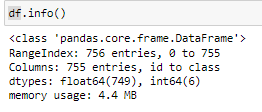
\includegraphics[width=0.5\textwidth]{imagens/datasetInfo.png}
    \caption{Informação geral acerca do Conjuntos de dados, incluindo tipo de variáveis.}
    \label{fig:datasetInfo}
\end{figure}

Uma parte sempre importante na análise do Conjunto de dados, é a verificação da existência da valores omissos. Na Figura \ref{fig:checkNulls} demonstra-se que não existe nenhum valor omisso no Conjunto de dados, em qualquer uma das suas \textit{features}. 

\begin{figure}[H]
    \centering
    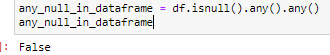
\includegraphics[width=0.5\textwidth]{imagens/checkNulls.png}
    \caption{Verificação de valores omissos no conjunto de dados.}
    \label{fig:checkNulls}
\end{figure}

Como se trata de um problema de classificação é importante a existência de um conjunto de dados balanceado. Tendo por base este pressuposto, analisou-se os atributos presentes na classe, sendo esta binária (0 ou 1), representado a inexistência ou existência de Doença de \textit{Parkinson}, respetivamente. Na Figura \ref{fig:checkClass}, verifica-se que a quantidade de registos da classe está desbalanceada, uma vez que esta apresenta cerca de 192 casos na \textit{label} 0, representante da não presença de \textit{Parkinson}, enquanto que apresenta 565 registos na \textit{label}, associada à doença de \textit{Parkinson}.

\begin{figure}[H]
    \centering
    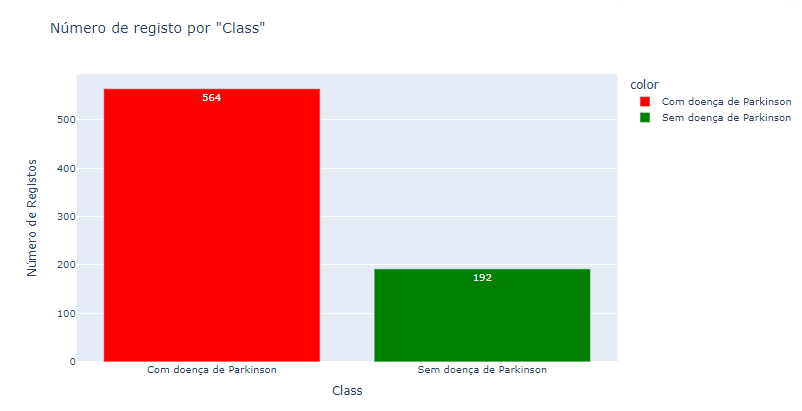
\includegraphics[width=1\textwidth]{imagens/classDistribution.png}
    \caption{Número de casos da não existência e da existência da doença de \textit{Parkinson}.}
    \label{fig:checkClass}
\end{figure}

Ainda na perspetiva de analisar o balanceamento do conjunto de dados, analisou-se a variável representativa do género dos pacientes, sendo esta binária (0 ou 1), representa indivíduos do sexo feminino e do sexo masculino, respetivamente. Na Figura \ref{fig:checkGender}, verifica-se que a quantidade de registos por género de encontra balanceado, verificando-se 366 indivíduos do sexo feminino e 490 indivíduos do sexo masculino.

\begin{figure}[H]
    \centering
    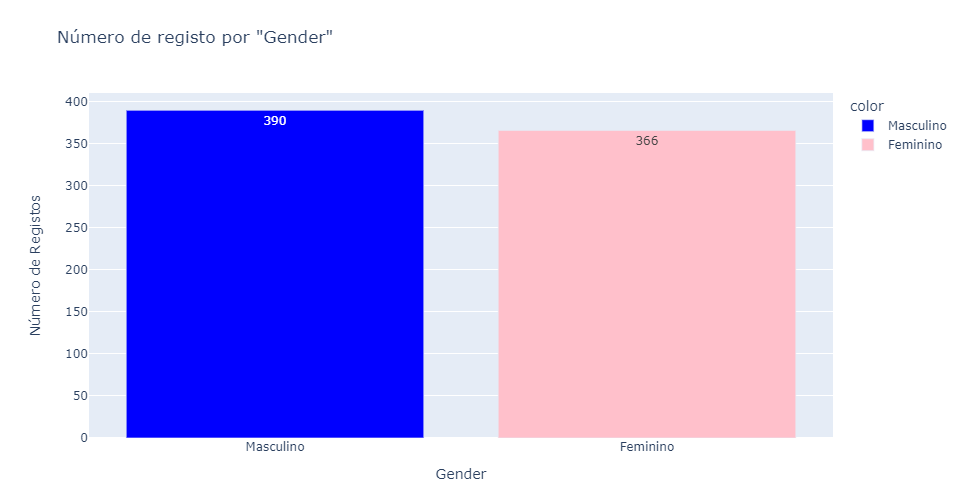
\includegraphics[width=1\textwidth]{imagens/GenderDistribution.png}
    \caption{Número de casos da indíviduos do sexo Feminino e do sexo Masculino.}
    \label{fig:checkGender}
\end{figure}

\section{Metodologias}

Ao nível do tratamento de Dados seguiram-se diversas abordagens, de forma a se puder estudar o problema de diversas formas. Inicialmente, verificou-se a não existência de valores omissos e a não existência de Variáveis categóricas, o que facilitou o processo de tratamento de dados, não sendo necessária a eliminação ou substituição dos valores omissos, bem como a realização de \textit{One-Hot Encoding} ou \textit{LabelEncoding} ao nível das variáveis categóricas.

Ainda neste sentido dividiu-se o problema em duas abordagens distintas: Utilização de todo o conjunto de dados e Divisão do conjunto de dados por género.

Apesar da divisão ou não existência de divisão de dados por género, a nível de Metodologia esta é semelhante no intuito geral, isto é, na etapa de pré-processamento dos conjuntos de dados, de divisão de conjunto de dados de treino e de teste, modelação através de diversas técnicas de \textit{Machine Learning}, otimização dos Hiperparâmetros e avaliação da performances dos diversos modelos com as Métricas, tal como se verifica na Figura \ref{fig:methodology}.

\begin{figure}[H]
    \centering
    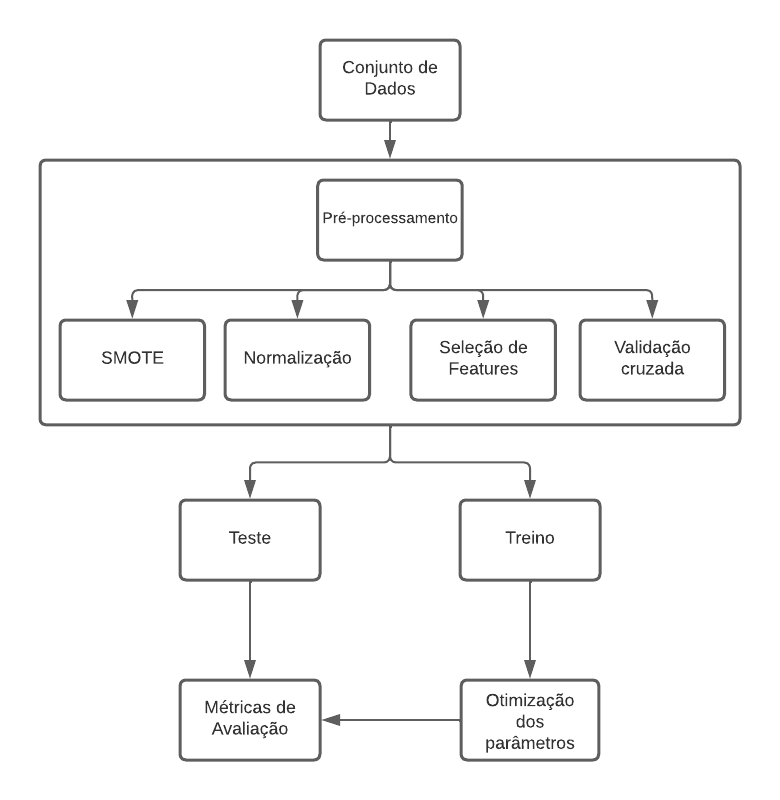
\includegraphics[width=0.8\textwidth]{imagens/metodologia.png}
    \caption{Metodologia aplicada.}
    \label{fig:methodology}
\end{figure}


\subsection{Conjunto de dados Completo}

Nesta abordagem utiliza-se o conjunto de dados completo como ponto inicial, sendo que mesmo dentro desta abordagens existem diversos teste que são realizados. 

Uma primeira abordagem, sendo uma espécie de \textit{baseline}, ou seja, sem grandes etapas de processamento de dados (apenas se procedeu com a eliminação da variável "id", uma vez que apenas é representativa da identificação do registo), foi através da utilização do conjunto de dados fornecido completo, ou seja, uma conjunto de dados desbalanceado, em que se realizou a etapa de Normalização através do \textit{MinMaxScaler}, não se realizaram algoritmos de seleção de features, sendo que se aplicaram 7 algoritmos distintos (\gls{SVM}, \Gls{RF}, \gls{NN}, \gls{NB}, \Gls{DT}, \Gls{XGBoost} e \gls{AdaBoost}), com Validação cruzada e otimização dos hiperparâmetros.

Uma vez que o Conjunto de dados Original apresente 752 \textit{features} e caso todas estas \textit{features} sejam utilizadas no processo de treino existe um aumento significativo no tempo de processamento, além de que pode resultar em problemas de \textit{features} duplicadas, \textit{features} efetivas, torna-se necessária a existência de diferentes técnicas de seleção de \textit{features}, que serão explicadas nas próximas abordagens.

Numa segunda abordagem, com o conjunto de dados desbalanceado, procedeu-se com a etapa de Normalização através do \textit{MinMaxScaler} e ao nível de seleção de \textit{features} utilizou-se a Correlação de \textit{Pearson}, removendo-se assim todas as \textit{features} com uma correlação superior a 0.8, resultando numa quantidade final de 262 \textit{features}.  Nesta abordagem testaram-se os mesmos 7 algoritmos com Validação Cruzada e Otimização dos Hiperparâmetros.

Numa terceira abordagem, ainda com o conjunto de dados desbalanceado, procedeu-se com a etapa de Normalização através do \textit{MinMaxScaler} e ao nível de seleção de \textit{features} utilizou-se a Correlação de \textit{Pearson} e o algoritmo de \gls{PCA}, removendo-se assim todas as \textit{features} com uma correlação superior a 0.8, resultando numa quantidade final de 262 \textit{features}, que através do \gls{PCA} reduziu-se para 111 \textit{features}.  Nesta abordagem testaram-se os mesmos 7 algoritmos com Validação Cruzada e Otimização dos Hiperparâmetros.

A quarta abordagem já apresenta um dataset balanceado através da utilização do algoritmo de \textit{SMOTE}, resultando num conjunto de dados com 1128 registos, sendo metade destes registos referentes a indivíduos sem a Doença de \textit{Parkinson} e outra metade referente a indivíduos com a Doença de \textit{Parkinson}. A importância deste balanceamento de dados é diretamente proporcional com a proporção de dados entre as duas diferentes \textit{labels} da classe está presenta na Tabela \ref{smotetable}.

\begin{table}[H]
\caption{Comparação entre Conjunto de dados Desbalanceado e Conjunto de dados balanceado}
\label{smotetable}
\centering
%% \tablesize{} %% You can specify the fontsize here, e.g., \tablesize{\footnotesize}. If commented out \small will be used.
\begin{tabular}{cccc}
\toprule
\textbf{\textit{Dataset}}	& \textbf{Número de casos de PD} &  \textbf{Número de casos sem PD} &\textbf{Total} \\
\midrule
Original & 564 & 192 & 756 \\
\gls{SMOTE} & 564 &	564 & 1128	\\
\bottomrule
\end{tabular}
\end{table}


A este conjunto de dados balanceado aplicou-se uma a etapa de Normalização através do \textit{MinMaxScaler}, não se realizaram algoritmos de seleção de features, sendo que se aplicaram 7 algoritmos distintos (\gls{SVM}, \Gls{RF}, \gls{NN}, \gls{NB}, \Gls{DT}, \Gls{XGBoost} e \gls{AdaBoost}), com Validação cruzada e otimização dos hiperparâmetros.

A quinta abordagem apresenta um dataset balanceado através da utilização do algoritmo de \textit{SMOTE}, resultando num conjunto de dados com 1128 registos, sendo metade destes registos referentes a indivíduos sem a Doença de \textit{Parkinson} e outra metade referente a indivíduos com a Doença de \textit{Parkinson}. A este conjunto de dados balanceado aplicou-se uma a etapa de Normalização através do \textit{MinMaxScaler} e uma redução das features através da eliminação das features com coeficiente de \textit{Pearson} superior a 0.8, sendo que se aplicaram 7 algoritmos distintos (\gls{SVM}, \Gls{RF}, \gls{NN}, \gls{NB}, \Gls{DT}, \Gls{XGBoost} e \gls{AdaBoost}), com Validação cruzada e otimização dos hiperparâmetros.

A sexta abordagem apresenta um dataset balanceado através da utilização do algoritmo de \textit{SMOTE}, resultando num conjunto de dados com 1128 registos, sendo metade destes registos referentes a indivíduos sem a Doença de \textit{Parkinson} e outra metade referente a indivíduos com a Doença de \textit{Parkinson}. A este conjunto de dados balanceado aplicou-se uma a etapa de Normalização através do \textit{MinMaxScaler} e uma redução das features através da eliminação das features com coeficiente de \textit{Pearson} superior a 0.8, resultando numa quantidade final de 262 \textit{features}, que através do \gls{PCA} reduziu-se para 111 \textit{features}. Por fim, aplicaram-se 7 algoritmos distintos (\gls{SVM}, \Gls{RF}, \gls{NN}, \gls{NB}, \Gls{DT}, \Gls{XGBoost} e \gls{AdaBoost}), com Validação cruzada e otimização dos hiperparâmetros.

A Sétima, oitava, nova, décima, décima-primeira e décima-segunda abordagem compreendem o estudo individual de cada um dos conjuntos de \textit{Features}, \textit{Baseline Features, Time Frequency Features, Vocal Fold Features, MFCCs features, Wavelet Features} e \textit{TQWT Features}, respetivamente. Inicialmente procedeu-se à divisão do Conjunto de dados entre as diferentes conjuntos de \textit{features}, sendo que este já se apresentava Balanceado com a utilização do \gls{SMOTE} e normalizado.

A décima-terceira abordagem diferenciou-se pela utilização da \textit{Feature Importance} do Algoritmo \gls{XGBoost} para a seleção de \textit{Features}, após o balanceamento e normalização do Conjunto de dados, de onde resultou um conjunto de dados final com 44 \textit{features}. Posteriormente, utilizou-se um \textit{Stacking Ensemble} como Classificador, com os algoritmos \gls{RF}, \Gls{GB}, \gls{SVM} e \gls{NN} como classificadores Base e dois diferentes algoritmos como classificador Meta (\gls{LR} e \gls{XGBoost}.

Na décima-quarta abordagem também se compreendeu a uma divisão do conjunto de dados nos diferentes conjuntos de \textit{Features}, \textit{Baseline Features, Time Frequency Features, Vocal Fold Features, MFCCs features, Wavelet Features} e \textit{TQWT Features}, respetivamente. Uma vez feita esta divisão, treinou-se individualmente cada um dos Conjuntos de \textit{Features} com o algoritmo \gls{RF} e as suas previsões serviram de \textit{input} para um algoritmo de \textit{Soft Voting Ensemble}.

Na décima-quinta abordagem, procedeu-se a um balanceamento do conjunto de dados e a uma normalização antes da seleção de \textit{Features} com o algoritmo de \gls{XGBoost}, o que resultou num conjunto de dados com 44 \textit{features}. Por fim, aplicaram-se 7 algoritmos distintos (\gls{SVM}, \Gls{RF}, \gls{NN}, \gls{NB}, \Gls{DT}, \Gls{XGBoost} e \gls{AdaBoost}), com Validação cruzada e otimização dos hiperparâmetros.

Na décima-sexta abordagem, procedeu-se a um balanceamento do conjunto de dados e a uma normalização antes da seleção de \textit{Features} com a utilização do \gls{VIF}, o que resultou num conjunto de dados com 125 \textit{features}. Posteriormente, utilizou-se um \textit{Stacking Ensemble} como Classificador, com os algoritmos \gls{NN}, \Gls{GB}, \gls{SVM} e \gls{XGBoost} como classificadores Base e o algoritmo de \gls{LR} como Classificador Meta.

Na décima-sétima abordagem, procedeu-se a um balanceamento do conjunto de dados e a uma normalização antes da seleção de \textit{Features} com a utilização do \gls{VIF}, o que resultou num conjunto de dados com 125 \textit{features}, ao qual foi aplicado posteriormente um \gls{PCA}, resultando num total de 60 \textit{features}. Posteriormente, utilizou-se um \textit{Stacking Ensemble} como Classificador, com os algoritmos \gls{NN}, \Gls{GB}, \gls{SVM} e \gls{XGBoost} como classificadores Base e o algoritmo de \gls{LR} como Classificador Meta.

Na décima-oitava abordagem, procedeu-se a um balanceamento do conjunto de dados e a uma normalização antes da seleção de \textit{Features} com a utilização do \gls{VIF}, o que resultou num conjunto de dados com 125 \textit{features}, das quais se selecionou 96 \textit{features} finais através da \textit{Feature Importance} do \gls{XGBoost}. Posteriormente, utilizou-se um \textit{Stacking Ensemble} como Classificador, com os algoritmos \gls{NN}, \Gls{GB}, \gls{SVM} e \gls{XGBoost} como classificadores Base e o algoritmo de \gls{LR} como Classificador Meta.

\subsection{Conjunto de dados dividido por género}

Numa outra abordagem, dividiu-se o conjunto de dados pelo seu género, procedendo-se ao seu treino e teste, de forma separada, sendo que a nível de etapas e Algoritmos utilizados o processo foi bastante semelhante ao processo com o conjunto de dados completo. A nível de objetivos pretendeu-se avaliar a possível influência ao nível de resultados quando estes estão agrupados pelo mesmo género.


\section{Análise dos Resultados}

\subsection{Conjunto de dados Completo}

Na Tabela \ref{tab:resultsAll} apresentam-se os resultados obtidos em estudo com diversas características de processamento e normalização dos dados, no caso em que se considera todo o conjunto de dados, isto é, não existindo uma diferenciação entre género. 

\begin{comment}
\begin{longtable}{|llllll|}
\caption{Análise de resultados com o conjunto de dados completo}
\label{tab:resultsAll}\\
\hline
\multicolumn{6}{|c|}{\textbf{Estudos}} \\ \hline
\endfirsthead
%
\endhead
%
\multicolumn{1}{|l|}{\textbf{Principais Características}} &
  \multicolumn{1}{l|}{\textbf{Algoritmos}} &
  \multicolumn{1}{l|}{\textbf{AUC}} &
  \multicolumn{1}{l|}{\textbf{F1}} &
  \multicolumn{1}{l|}{\textbf{ACC}} &
  \textbf{Tempo} \\ \hline
\multicolumn{1}{|l|}{} &
  \multicolumn{1}{l|}{SVM} &
  \multicolumn{1}{l|}{0.772} &
  \multicolumn{1}{l|}{0.926} &
  \multicolumn{1}{l|}{0.882} &
  10.082 \\ \cline{2-6} 
\multicolumn{1}{|l|}{} &
  \multicolumn{1}{l|}{Random Forest} &
  \multicolumn{1}{l|}{0.754} &
  \multicolumn{1}{l|}{0.908} &
  \multicolumn{1}{l|}{0.855} &
  161.787 \\ \cline{2-6} 
\multicolumn{1}{|l|}{} &
  \multicolumn{1}{l|}{KNN} &
  \multicolumn{1}{l|}{0.860} &
  \multicolumn{1}{l|}{0.930} &
  \multicolumn{1}{l|}{0.895} &
  2.313 \\ \cline{2-6} 
\multicolumn{1}{|l|}{} &
  \multicolumn{1}{l|}{Naive Bayes} &
  \multicolumn{1}{l|}{0.741} &
  \multicolumn{1}{l|}{0.862} &
  \multicolumn{1}{l|}{0.796} &
  0.595 \\ \cline{2-6} 
\multicolumn{1}{|l|}{} &
  \multicolumn{1}{l|}{Decision Tree} &
  \multicolumn{1}{l|}{0.706} &
  \multicolumn{1}{l|}{0.833} &
  \multicolumn{1}{l|}{0.757} &
  6.714 \\ \cline{2-6} 
\multicolumn{1}{|l|}{} &
  \multicolumn{1}{l|}{XGBoost} &
  \multicolumn{1}{l|}{0.816} &
  \multicolumn{1}{l|}{0.933} &
  \multicolumn{1}{l|}{0.895} &
  532.757 \\ \cline{2-6} 
\multicolumn{1}{|l|}{\multirow{-7}{*}{\begin{tabular}[c]{@{}l@{}}Conjunto de dados desbalanceado, \\ com MinMaxScaler com todas as \\ features, 5 fold Cross-Validation e \\ GridSearch\end{tabular}}} &
  \multicolumn{1}{l|}{AdaBoost} &
  \multicolumn{1}{l|}{0.838} &
  \multicolumn{1}{l|}{0.936} &
  \multicolumn{1}{l|}{0.901} &
  192.909 \\ \hline
\multicolumn{1}{|l|}{} &
  \multicolumn{1}{l|}{SVM} &
  \multicolumn{1}{l|}{0.741} &
  \multicolumn{1}{l|}{0.905} &
  \multicolumn{1}{l|}{0.849} &
  4.335 \\ \cline{2-6} 
\multicolumn{1}{|l|}{} &
  \multicolumn{1}{l|}{Random Forest} &
  \multicolumn{1}{l|}{0.732} &
  \multicolumn{1}{l|}{0.915} &
  \multicolumn{1}{l|}{0.862} &
  103.169 \\ \cline{2-6} 
\multicolumn{1}{|l|}{} &
  \multicolumn{1}{l|}{KNN} &
  \multicolumn{1}{l|}{0.890} &
  \multicolumn{1}{l|}{0.962} &
  \multicolumn{1}{l|}{0.941} &
  1.098 \\ \cline{2-6} 
\multicolumn{1}{|l|}{} &
  \multicolumn{1}{l|}{Naive Bayes} &
  \multicolumn{1}{l|}{0.732} &
  \multicolumn{1}{l|}{0.828} &
  \multicolumn{1}{l|}{0.757} &
  0.233 \\ \cline{2-6} 
\multicolumn{1}{|l|}{} &
  \multicolumn{1}{l|}{Decision Tree} &
  \multicolumn{1}{l|}{0.741} &
  \multicolumn{1}{l|}{0.850} &
  \multicolumn{1}{l|}{0.783} &
  1.778 \\ \cline{2-6} 
\multicolumn{1}{|l|}{} &
  \multicolumn{1}{l|}{XGBoost} &
  \multicolumn{1}{l|}{0.750} &
  \multicolumn{1}{l|}{0.914} &
  \multicolumn{1}{l|}{0.862} &
  133.619 \\ \cline{2-6} 
\multicolumn{1}{|l|}{\multirow{-7}{*}{\begin{tabular}[c]{@{}l@{}}Conjunto de dados desbalanceado, \\ com MinMaxScaler com remoção\\ de variáveis com correlação superior\\ a 0.8 (262 features),  5 fold \\ Cross-Validation e  GridSearch\end{tabular}}} &
  \multicolumn{1}{l|}{AdaBoost} &
  \multicolumn{1}{l|}{0.763} &
  \multicolumn{1}{l|}{0.908} &
  \multicolumn{1}{l|}{0.855} &
  39.323 \\ \hline
\multicolumn{1}{|l|}{} &
  \multicolumn{1}{l|}{SVM} &
  \multicolumn{1}{l|}{0.794} &
  \multicolumn{1}{l|}{0.929} &
  \multicolumn{1}{l|}{0.888} &
  1.385 \\ \cline{2-6} 
\multicolumn{1}{|l|}{} &
  \multicolumn{1}{l|}{Random Forest} &
  \multicolumn{1}{l|}{0.614} &
  \multicolumn{1}{l|}{0.883} &
  \multicolumn{1}{l|}{0.803} &
  39.256 \\ \cline{2-6} 
\multicolumn{1}{|l|}{} &
  \multicolumn{1}{l|}{KNN} &
  \multicolumn{1}{l|}{0.833} &
  \multicolumn{1}{l|}{0.941} &
  \multicolumn{1}{l|}{0.908} &
  0.519 \\ \cline{2-6} 
\multicolumn{1}{|l|}{} &
  \multicolumn{1}{l|}{Naive Bayes} &
  \multicolumn{1}{l|}{0.658} &
  \multicolumn{1}{l|}{0.823} &
  \multicolumn{1}{l|}{0.737} &
  0.154 \\ \cline{2-6} 
\multicolumn{1}{|l|}{} &
  \multicolumn{1}{l|}{Decision Tree} &
  \multicolumn{1}{l|}{0.724} &
  \multicolumn{1}{l|}{0.896} &
  \multicolumn{1}{l|}{0.836} &
  1.030 \\ \cline{2-6} 
\multicolumn{1}{|l|}{} &
  \multicolumn{1}{l|}{XGBoost} &
  \multicolumn{1}{l|}{0.750} &
  \multicolumn{1}{l|}{0.914} &
  \multicolumn{1}{l|}{0.862} &
  68.663 \\ \cline{2-6} 
\multicolumn{1}{|l|}{\multirow{-7}{*}{\begin{tabular}[c]{@{}l@{}}Conjunto de dados desbalanceado, \\ com MinMaxScaler com remoção\\ de variáveis com correlação superior\\ a 0.8 e PCA,  5 fold \\ Cross-Validation e  GridSearch\end{tabular}}} &
  \multicolumn{1}{l|}{AdaBoost} &
  \multicolumn{1}{l|}{0.724} &
  \multicolumn{1}{l|}{0.865} &
  \multicolumn{1}{l|}{0.796} &
  22.221 \\ \hline
\multicolumn{1}{|l|}{} &
  \multicolumn{1}{l|}{SVM} &
  \multicolumn{1}{l|}{0.948} &
  \multicolumn{1}{l|}{0.947} &
  \multicolumn{1}{l|}{0.947} &
  29.770 \\ \cline{2-6} 
\multicolumn{1}{|l|}{} &
  \multicolumn{1}{l|}{Random Forest} &
  \multicolumn{1}{l|}{0.931} &
  \multicolumn{1}{l|}{0.929} &
  \multicolumn{1}{l|}{0.929} &
  230.486 \\ \cline{2-6} 
\multicolumn{1}{|l|}{} &
  \multicolumn{1}{l|}{KNN} &
  \multicolumn{1}{l|}{0.936} &
  \multicolumn{1}{l|}{0.932} &
  \multicolumn{1}{l|}{0.934} &
  15.969 \\ \cline{2-6} 
\multicolumn{1}{|l|}{} &
  \multicolumn{1}{l|}{Naive Bayes} &
  \multicolumn{1}{l|}{0.792} &
  \multicolumn{1}{l|}{0.798} &
  \multicolumn{1}{l|}{0.792} &
  2.279 \\ \cline{2-6} 
\multicolumn{1}{|l|}{} &
  \multicolumn{1}{l|}{Decision Tree} &
  \multicolumn{1}{l|}{0.890} &
  \multicolumn{1}{l|}{0.890} &
  \multicolumn{1}{l|}{0.889} &
  16.509 \\ \cline{2-6} 
\multicolumn{1}{|l|}{} &
  \multicolumn{1}{l|}{XGBoost} &
  \multicolumn{1}{l|}{0.957} &
  \multicolumn{1}{l|}{0.956} &
  \multicolumn{1}{l|}{0.956} &
  671.184 \\ \cline{2-6} 
\multicolumn{1}{|l|}{\multirow{-7}{*}{\begin{tabular}[c]{@{}l@{}}Conjunto de dados balanceado com \\ SMOTE,  MinMaxScaler, 5 fold \\ Cross-Validation e  GridSearch\end{tabular}}} &
  \multicolumn{1}{l|}{AdaBoost} &
  \multicolumn{1}{l|}{0.921} &
  \multicolumn{1}{l|}{0.921} &
  \multicolumn{1}{l|}{0.920} &
  275.578 \\ \hline
\multicolumn{1}{|l|}{} &
  \multicolumn{1}{l|}{SVM} &
  \multicolumn{1}{l|}{0.926} &
  \multicolumn{1}{l|}{0.924} &
  \multicolumn{1}{l|}{0.925} &
  0.505 \\ \cline{2-6} 
\multicolumn{1}{|l|}{} &
  \multicolumn{1}{l|}{Random Forest} &
  \multicolumn{1}{l|}{0.930} &
  \multicolumn{1}{l|}{0.930} &
  \multicolumn{1}{l|}{0.929} &
  85.232 \\ \cline{2-6} 
\multicolumn{1}{|l|}{} &
  \multicolumn{1}{l|}{KNN} &
  \multicolumn{1}{l|}{0.953} &
  \multicolumn{1}{l|}{0.951} &
  \multicolumn{1}{l|}{0.951} &
  1.476 \\ \cline{2-6} 
\multicolumn{1}{|l|}{} &
  \multicolumn{1}{l|}{Naive Bayes} &
  \multicolumn{1}{l|}{0.813} &
  \multicolumn{1}{l|}{0.794} &
  \multicolumn{1}{l|}{0.810} &
  0.258 \\ \cline{2-6} 
\multicolumn{1}{|l|}{} &
  \multicolumn{1}{l|}{Decision Tree} &
  \multicolumn{1}{l|}{0.869} &
  \multicolumn{1}{l|}{0.866} &
  \multicolumn{1}{l|}{0.867} &
  2.689 \\ \cline{2-6} 
\multicolumn{1}{|l|}{} &
  \multicolumn{1}{l|}{XGBoost} &
  \multicolumn{1}{l|}{0.944} &
  \multicolumn{1}{l|}{0.943} &
  \multicolumn{1}{l|}{0.942} &
  152.633 \\ \cline{2-6} 
\multicolumn{1}{|l|}{\multirow{-7}{*}{\begin{tabular}[c]{@{}l@{}}Conjunto de dados balanceado com \\ SMOTE, remoção de variáveis com\\ correlação superior a 0.8 (263),\\  MinMaxScaler, 5 fold Cross-Validation \\ e  GridSearch\end{tabular}}} &
  \multicolumn{1}{l|}{AdaBoost} &
  \multicolumn{1}{l|}{0.930} &
  \multicolumn{1}{l|}{0.930} &
  \multicolumn{1}{l|}{0.929} &
  75.791 \\ \hline
\multicolumn{1}{|l|}{} &
  \multicolumn{1}{l|}{SVM} &
  \multicolumn{1}{l|}{0.952} &
  \multicolumn{1}{l|}{0.952} &
  \multicolumn{1}{l|}{0.951} &
  3.269 \\ \cline{2-6} 
\multicolumn{1}{|l|}{} &
  \multicolumn{1}{l|}{Random Forest} &
  \multicolumn{1}{l|}{0.890} &
  \multicolumn{1}{l|}{0.891} &
  \multicolumn{1}{l|}{0.889} &
  67.916 \\ \cline{2-6} 
\multicolumn{1}{|l|}{} &
  \multicolumn{1}{l|}{KNN} &
  \multicolumn{1}{l|}{0.910} &
  \multicolumn{1}{l|}{0.901} &
  \multicolumn{1}{l|}{0.907} &
  0.935 \\ \cline{2-6} 
\multicolumn{1}{|l|}{} &
  \multicolumn{1}{l|}{Naive Bayes} &
  \multicolumn{1}{l|}{0.792} &
  \multicolumn{1}{l|}{0.800} &
  \multicolumn{1}{l|}{0.792} &
  0.170 \\ \cline{2-6} 
\multicolumn{1}{|l|}{} &
  \multicolumn{1}{l|}{Decision Tree} &
  \multicolumn{1}{l|}{0.839} &
  \multicolumn{1}{l|}{0.829} &
  \multicolumn{1}{l|}{0.836} &
  1.487 \\ \cline{2-6} 
\multicolumn{1}{|l|}{} &
  \multicolumn{1}{l|}{XGBoost} &
  \multicolumn{1}{l|}{0.913} &
  \multicolumn{1}{l|}{0.910} &
  \multicolumn{1}{l|}{0.912} &
  78.830 \\ \cline{2-6} 
\multicolumn{1}{|l|}{\multirow{-7}{*}{\begin{tabular}[c]{@{}l@{}}Conjunto de dados balanceado com \\ SMOTE, remoção de variáveis com\\ correlação superior a 0.8 e PCA,\\  MinMaxScaler, 5 fold Cross-Validation \\ e  GridSearch\end{tabular}}} &
  \multicolumn{1}{l|}{AdaBoost} &
  \multicolumn{1}{l|}{0.872} &
  \multicolumn{1}{l|}{0.873} &
  \multicolumn{1}{l|}{0.872} &
  35.929 \\ \hline
\multicolumn{1}{|l|}{} &
  \multicolumn{1}{l|}{SVM} &
  \multicolumn{1}{l|}{0.816} &
  \multicolumn{1}{l|}{0.809} &
  \multicolumn{1}{l|}{0.814} &
  2.922 \\ \cline{2-6} 
\multicolumn{1}{|l|}{} &
  \multicolumn{1}{l|}{Random Forest} &
  \multicolumn{1}{l|}{0.837} &
  \multicolumn{1}{l|}{0.834} &
  \multicolumn{1}{l|}{0.836} &
  53.365 \\ \cline{2-6} 
\multicolumn{1}{|l|}{} &
  \multicolumn{1}{l|}{KNN} &
  \multicolumn{1}{l|}{0.791} &
  \multicolumn{1}{l|}{0.769} &
  \multicolumn{1}{l|}{0.788} &
  0.684 \\ \cline{2-6} 
\multicolumn{1}{|l|}{} &
  \multicolumn{1}{l|}{Naive Bayes} &
  \multicolumn{1}{l|}{0.630} &
  \multicolumn{1}{l|}{0.555} &
  \multicolumn{1}{l|}{0.624} &
  0.110 \\ \cline{2-6} 
\multicolumn{1}{|l|}{} &
  \multicolumn{1}{l|}{Decision Tree} &
  \multicolumn{1}{l|}{0.816} &
  \multicolumn{1}{l|}{0.807} &
  \multicolumn{1}{l|}{0.814} &
  0.447 \\ \cline{2-6} 
\multicolumn{1}{|l|}{} &
  \multicolumn{1}{l|}{XGBoost} &
  \multicolumn{1}{l|}{0.869} &
  \multicolumn{1}{l|}{0.865} &
  \multicolumn{1}{l|}{0.867} &
  23.198 \\ \cline{2-6} 
\multicolumn{1}{|l|}{\multirow{-7}{*}{\begin{tabular}[c]{@{}l@{}}Conjunto de dados balanceado com \\ SMOTE,  MinMaxScaler, \\ 5 fold Cross-Validation  e  GridSearch. \\ Utilização de apenas as baseline features\end{tabular}}} &
  \multicolumn{1}{l|}{AdaBoost} &
  \multicolumn{1}{l|}{0.841} &
  \multicolumn{1}{l|}{0.845} &
  \multicolumn{1}{l|}{0.841} &
  16.644 \\ \hline
\multicolumn{1}{|l|}{} &
  \multicolumn{1}{l|}{SVM} &
  \multicolumn{1}{l|}{0.808} &
  \multicolumn{1}{l|}{0.796} &
  \multicolumn{1}{l|}{0.805} &
  2.981 \\ \cline{2-6} 
\multicolumn{1}{|l|}{} &
  \multicolumn{1}{l|}{Random Forest} &
  \multicolumn{1}{l|}{0.871} &
  \multicolumn{1}{l|}{0.858} &
  \multicolumn{1}{l|}{0.867} &
  47.341 \\ \cline{2-6} 
\multicolumn{1}{|l|}{} &
  \multicolumn{1}{l|}{KNN} &
  \multicolumn{1}{l|}{0.827} &
  \multicolumn{1}{l|}{0.806} &
  \multicolumn{1}{l|}{0.823} &
  0.568 \\ \cline{2-6} 
\multicolumn{1}{|l|}{} &
  \multicolumn{1}{l|}{Naive Bayes} &
  \multicolumn{1}{l|}{0.742} &
  \multicolumn{1}{l|}{0.760} &
  \multicolumn{1}{l|}{0.743} &
  0.127 \\ \cline{2-6} 
\multicolumn{1}{|l|}{} &
  \multicolumn{1}{l|}{Decision Tree} &
  \multicolumn{1}{l|}{0.786} &
  \multicolumn{1}{l|}{0.772} &
  \multicolumn{1}{l|}{0.783} &
  0.319 \\ \cline{2-6} 
\multicolumn{1}{|l|}{} &
  \multicolumn{1}{l|}{XGBoost} &
  \multicolumn{1}{l|}{0.871} &
  \multicolumn{1}{l|}{0.858} &
  \multicolumn{1}{l|}{0.867} &
  15.379 \\ \cline{2-6} 
\multicolumn{1}{|l|}{\multirow{-7}{*}{\begin{tabular}[c]{@{}l@{}}Conjunto de dados balanceado com \\ SMOTE,  MinMaxScaler, \\ 5 fold Cross-Validation  e  GridSearch. \\ Utilização de apenas as Time\\ Frequency features\end{tabular}}} &
  \multicolumn{1}{l|}{AdaBoost} &
  \multicolumn{1}{l|}{0.773} &
  \multicolumn{1}{l|}{0.857} &
  \multicolumn{1}{l|}{0.770} &
  12.209 \\ \hline
\multicolumn{1}{|l|}{} &
  \multicolumn{1}{l|}{SVM} &
  \multicolumn{1}{l|}{0.776} &
  \multicolumn{1}{l|}{0.767} &
  \multicolumn{1}{l|}{0.774} &
  3.070 \\ \cline{2-6} 
\multicolumn{1}{|l|}{} &
  \multicolumn{1}{l|}{Random Forest} &
  \multicolumn{1}{l|}{0.895} &
  \multicolumn{1}{l|}{0.895} &
  \multicolumn{1}{l|}{0.894} &
  53.097 \\ \cline{2-6} 
\multicolumn{1}{|l|}{} &
  \multicolumn{1}{l|}{KNN} &
  \multicolumn{1}{l|}{0.832} &
  \multicolumn{1}{l|}{0.810} &
  \multicolumn{1}{l|}{0.827} &
  0.633 \\ \cline{2-6} 
\multicolumn{1}{|l|}{} &
  \multicolumn{1}{l|}{Naive Bayes} &
  \multicolumn{1}{l|}{0.665} &
  \multicolumn{1}{l|}{0.699} &
  \multicolumn{1}{l|}{0.668} &
  0.126 \\ \cline{2-6} 
\multicolumn{1}{|l|}{} &
  \multicolumn{1}{l|}{Decision Tree} &
  \multicolumn{1}{l|}{0.692} &
  \multicolumn{1}{l|}{0.685} &
  \multicolumn{1}{l|}{0.690} &
  0.478 \\ \cline{2-6} 
\multicolumn{1}{|l|}{} &
  \multicolumn{1}{l|}{XGBoost} &
  \multicolumn{1}{l|}{0.904} &
  \multicolumn{1}{l|}{0.902} &
  \multicolumn{1}{l|}{0.903} &
  25.688 \\ \cline{2-6} 
\multicolumn{1}{|l|}{\multirow{-7}{*}{\begin{tabular}[c]{@{}l@{}}Conjunto de dados balanceado com \\ SMOTE,  MinMaxScaler, \\ 5 fold Cross-Validation  e  GridSearch. \\ Utilização de apenas as Vocal\\ Fold features\end{tabular}}} &
  \multicolumn{1}{l|}{AdaBoost} &
  \multicolumn{1}{l|}{0.740} &
  \multicolumn{1}{l|}{0.740} &
  \multicolumn{1}{l|}{0.739} &
  18.485 \\ \hline
\multicolumn{1}{|l|}{} &
  \multicolumn{1}{l|}{SVM} &
  \multicolumn{1}{l|}{0.939} &
  \multicolumn{1}{l|}{0.938} &
  \multicolumn{1}{l|}{0.938} &
  3.546 \\ \cline{2-6} 
\multicolumn{1}{|l|}{} &
  \multicolumn{1}{l|}{Random Forest} &
  \multicolumn{1}{l|}{0.887} &
  \multicolumn{1}{l|}{0.883} &
  \multicolumn{1}{l|}{0.885} &
  81.300 \\ \cline{2-6} 
\multicolumn{1}{|l|}{} &
  \multicolumn{1}{l|}{KNN} &
  \multicolumn{1}{l|}{0.833} &
  \multicolumn{1}{l|}{0.802} &
  \multicolumn{1}{l|}{0.827} &
  0.965 \\ \cline{2-6} 
\multicolumn{1}{|l|}{} &
  \multicolumn{1}{l|}{Naive Bayes} &
  \multicolumn{1}{l|}{0.729} &
  \multicolumn{1}{l|}{0.659} &
  \multicolumn{1}{l|}{0.721} &
  0.165 \\ \cline{2-6} 
\multicolumn{1}{|l|}{} &
  \multicolumn{1}{l|}{Decision Tree} &
  \multicolumn{1}{l|}{0.852} &
  \multicolumn{1}{l|}{0.843} &
  \multicolumn{1}{l|}{0.850} &
  1.461 \\ \cline{2-6} 
\multicolumn{1}{|l|}{} &
  \multicolumn{1}{l|}{XGBoost} &
  \multicolumn{1}{l|}{0.887} &
  \multicolumn{1}{l|}{0.883} &
  \multicolumn{1}{l|}{0.885} &
  55.515 \\ \cline{2-6} 
\multicolumn{1}{|l|}{\multirow{-7}{*}{\begin{tabular}[c]{@{}l@{}}Conjunto de dados balanceado com \\ SMOTE,  MinMaxScaler, \\ 5 fold Cross-Validation  e  GridSearch. \\ Utilização de apenas as MFCCs\\ features\end{tabular}}} &
  \multicolumn{1}{l|}{AdaBoost} &
  \multicolumn{1}{l|}{0.891} &
  \multicolumn{1}{l|}{0.888} &
  \multicolumn{1}{l|}{0.889} &
  30.739 \\ \hline
\multicolumn{1}{|l|}{} &
  \multicolumn{1}{l|}{SVM} &
  \multicolumn{1}{l|}{0.659} &
  \multicolumn{1}{l|}{0.672} &
  \multicolumn{1}{l|}{0.659} &
  5.464 \\ \cline{2-6} 
\multicolumn{1}{|l|}{} &
  \multicolumn{1}{l|}{Random Forest} &
  \multicolumn{1}{l|}{0.845} &
  \multicolumn{1}{l|}{0.848} &
  \multicolumn{1}{l|}{0.845} &
  101.497 \\ \cline{2-6} 
\multicolumn{1}{|l|}{} &
  \multicolumn{1}{l|}{KNN} &
  \multicolumn{1}{l|}{0.789} &
  \multicolumn{1}{l|}{0.749} &
  \multicolumn{1}{l|}{0.783} &
  1.496 \\ \cline{2-6} 
\multicolumn{1}{|l|}{} &
  \multicolumn{1}{l|}{Naive Bayes} &
  \multicolumn{1}{l|}{0.651} &
  \multicolumn{1}{l|}{0.695} &
  \multicolumn{1}{l|}{0.655} &
  0.278 \\ \cline{2-6} 
\multicolumn{1}{|l|}{} &
  \multicolumn{1}{l|}{Decision Tree} &
  \multicolumn{1}{l|}{0.744} &
  \multicolumn{1}{l|}{0.748} &
  \multicolumn{1}{l|}{0.743} &
  2.956 \\ \cline{2-6} 
\multicolumn{1}{|l|}{} &
  \multicolumn{1}{l|}{XGBoost} &
  \multicolumn{1}{l|}{0.828} &
  \multicolumn{1}{l|}{0.830} &
  \multicolumn{1}{l|}{0.827} &
  132.535 \\ \cline{2-6} 
\multicolumn{1}{|l|}{\multirow{-7}{*}{\begin{tabular}[c]{@{}l@{}}Conjunto de dados balanceado com \\ SMOTE,  MinMaxScaler, \\ 5 fold Cross-Validation  e  GridSearch. \\ Utilização de apenas as Wavelet\\ features\end{tabular}}} &
  \multicolumn{1}{l|}{AdaBoost} &
  \multicolumn{1}{l|}{0.783} &
  \multicolumn{1}{l|}{0.788} &
  \multicolumn{1}{l|}{0.783} &
  74.969 \\ \hline
\multicolumn{1}{|l|}{} &
  \multicolumn{1}{l|}{SVM} &
  \multicolumn{1}{l|}{0.659} &
  \multicolumn{1}{l|}{0.672} &
  \multicolumn{1}{l|}{0.659} &
  5.464 \\ \cline{2-6} 
\multicolumn{1}{|l|}{} &
  \multicolumn{1}{l|}{Random Forest} &
  \multicolumn{1}{l|}{0.845} &
  \multicolumn{1}{l|}{0.848} &
  \multicolumn{1}{l|}{0.845} &
  101.597 \\ \cline{2-6} 
\multicolumn{1}{|l|}{} &
  \multicolumn{1}{l|}{KNN} &
  \multicolumn{1}{l|}{0.780} &
  \multicolumn{1}{l|}{0.749} &
  \multicolumn{1}{l|}{0.783} &
  1.496 \\ \cline{2-6} 
\multicolumn{1}{|l|}{} &
  \multicolumn{1}{l|}{Naive Bayes} &
  \multicolumn{1}{l|}{0.651} &
  \multicolumn{1}{l|}{0.695} &
  \multicolumn{1}{l|}{0.655} &
  0.278 \\ \cline{2-6} 
\multicolumn{1}{|l|}{} &
  \multicolumn{1}{l|}{Decision Tree} &
  \multicolumn{1}{l|}{0.744} &
  \multicolumn{1}{l|}{0.748} &
  \multicolumn{1}{l|}{0.743} &
  2.956 \\ \cline{2-6} 
\multicolumn{1}{|l|}{} &
  \multicolumn{1}{l|}{XGBoost} &
  \multicolumn{1}{l|}{0.828} &
  \multicolumn{1}{l|}{0.830} &
  \multicolumn{1}{l|}{0.827} &
  132.535 \\ \cline{2-6} 
\multicolumn{1}{|l|}{\multirow{-7}{*}{\begin{tabular}[c]{@{}l@{}}Conjunto de dados balanceado com \\ SMOTE,  MinMaxScaler, \\ 5 fold Cross-Validation  e  GridSearch. \\ Utilização de apenas as TQWT\\ features\end{tabular}}} &
  \multicolumn{1}{l|}{AdaBoost} &
  \multicolumn{1}{l|}{0.783} &
  \multicolumn{1}{l|}{0.788} &
  \multicolumn{1}{l|}{0.783} &
  74.969 \\ \hline
\multicolumn{1}{|l|}{} &
  \multicolumn{1}{l|}{\begin{tabular}[c]{@{}l@{}}Essemble Stacking:  \\ LR como\\ Classificador Meta\end{tabular}} &
  \multicolumn{1}{l|}{0.983} &
  \multicolumn{1}{l|}{0.983} &
  \multicolumn{1}{l|}{0.982} &
  70.497 \\ \cline{2-6} 
\multicolumn{1}{|l|}{\multirow{-5}{*}{\begin{tabular}[c]{@{}l@{}}Conjunto de dados balanceado com \\ SMOTE,  MinMaxScaler, feature\\ selection com XGBoost, 5 fold \\ Cross-Validation e  GridSearch. \\ RF, GB, SVM e KNN como\\ Classificadores Base\end{tabular}}} &
  \multicolumn{1}{l|}{\begin{tabular}[c]{@{}l@{}}Essemble Stacking:  \\ XGBoost como\\ Classificador Meta\end{tabular}} &
  \multicolumn{1}{l|}{0.987} &
  \multicolumn{1}{l|}{0.987} &
  \multicolumn{1}{l|}{0.987} &
  71.723 \\ \hline
\multicolumn{1}{|l|}{\begin{tabular}[c]{@{}l@{}}Conjunto de dados balanceado com \\ SMOTE e MinMaxScaler. RF aplicado\\ em cada conjunto de features e as \\ previsões são utilizadas no Voting\\ Ensemble\end{tabular}} &
  \multicolumn{1}{l|}{Voting Ensemble} &
  \multicolumn{1}{l|}{0.909} &
  \multicolumn{1}{l|}{0.906} &
  \multicolumn{1}{l|}{0.907} &
  0.854 \\ \hline
\multicolumn{1}{|l|}{} &
  \multicolumn{1}{l|}{SVM} &
  \multicolumn{1}{l|}{0.890} &
  \multicolumn{1}{l|}{0.890} &
  \multicolumn{1}{l|}{0.889} &
  3.431 \\ \cline{2-6} 
\multicolumn{1}{|l|}{} &
  \multicolumn{1}{l|}{Random Forest} &
  \multicolumn{1}{l|}{0.922} &
  \multicolumn{1}{l|}{0.919} &
  \multicolumn{1}{l|}{0.920} &
  60.663 \\ \cline{2-6} 
\multicolumn{1}{|l|}{} &
  \multicolumn{1}{l|}{KNN} &
  \multicolumn{1}{l|}{0.918} &
  \multicolumn{1}{l|}{0.912} &
  \multicolumn{1}{l|}{0.916} &
  0.799 \\ \cline{2-6} 
\multicolumn{1}{|l|}{} &
  \multicolumn{1}{l|}{Naive Bayes} &
  \multicolumn{1}{l|}{0.791} &
  \multicolumn{1}{l|}{0.800} &
  \multicolumn{1}{l|}{0.792} &
  0.139 \\ \cline{2-6} 
\multicolumn{1}{|l|}{} &
  \multicolumn{1}{l|}{Decision Tree} &
  \multicolumn{1}{l|}{0.865} &
  \multicolumn{1}{l|}{0.858} &
  \multicolumn{1}{l|}{0.863} &
  0.908 \\ \cline{2-6} 
\multicolumn{1}{|l|}{} &
  \multicolumn{1}{l|}{XGBoost} &
  \multicolumn{1}{l|}{0.935} &
  \multicolumn{1}{l|}{0.934} &
  \multicolumn{1}{l|}{0.934} &
  35.416 \\ \cline{2-6} 
\multicolumn{1}{|l|}{\multirow{-7}{*}{\begin{tabular}[c]{@{}l@{}}Conjunto de dados balanceado com \\ SMOTE,  MinMaxScaler, feature\\ selection com XGBoost, 5 fold \\ Cross-Validation e  GridSearch.\end{tabular}}} &
  \multicolumn{1}{l|}{AdaBoost} &
  \multicolumn{1}{l|}{0.881} &
  \multicolumn{1}{l|}{0.881} &
  \multicolumn{1}{l|}{0.881} &
  26.767 \\ \hline
  \multicolumn{1}{|l|}{\begin{tabular}[c]{@{}l@{}}Conjunto de dados balanceado com \\ \gls{SMOTE} e \textit{MinMaxScaler}, redução de \\\textit{Features} através da utilização do \\índice de \gls{VIF} para 125 \textit{features}, 5 \textit{fold} \\ \textit{Cross-Validation} e \textit{GridSearch}.\\ \Gls{NN}, \gls{GB}, \gls{SVM} e \gls{XGBoost} como\\ Classificadores Base\end{tabular}} &
  \multicolumn{1}{l|}{\begin{tabular}[c]{@{}l@{}}\textit{Ensemble Stacking}:  \\ \gls{LR} como\\ Classificador Meta\end{tabular}} &
  \multicolumn{1}{l|}{0.978} &
  \multicolumn{1}{l|}{0.979} &
  \multicolumn{1}{l|}{0.978} &
  203.329 \\ \hline
   \multicolumn{1}{|l|}{\begin{tabular}[c]{@{}l@{}}Conjunto de dados balanceado com \\ \gls{SMOTE} e \textit{MinMaxScaler}, redução de \\\textit{Features} através da utilização do \\índice de \gls{VIF} e \gls{PCA}, 5 \textit{fold} \\ \textit{Cross-Validation} e \textit{GridSearch}.\\ \Gls{NN}, \gls{GB}, \gls{SVM} e \gls{XGBoost} como\\ Classificadores Base\end{tabular}} &
  \multicolumn{1}{l|}{\begin{tabular}[c]{@{}l@{}}\textit{Ensemble Stacking}:  \\ \gls{LR} como\\ Classificador Meta\end{tabular}} &
  \multicolumn{1}{l|}{0.973} &
  \multicolumn{1}{l|}{0.974} &
  \multicolumn{1}{l|}{0.973} &
  92.953 \\ \hline
   \multicolumn{1}{|l|}{\begin{tabular}[c]{@{}l@{}}Conjunto de dados balanceado com \\ \gls{SMOTE} e \textit{MinMaxScaler}, redução de \\\textit{Features} através da utilização do \\índice de \gls{VIF} e \gls{XGBoost} \textit{Feature}\\\textit{Importance}  para 96 \textit{features}, 5 \textit{fold} \\ \textit{Cross-Validation} e \textit{GridSearch}.\\ \Gls{NN}, \gls{GB}, \gls{SVM} e \gls{XGBoost} como\\ Classificadores Base\end{tabular}} &
  \multicolumn{1}{l|}{\begin{tabular}[c]{@{}l@{}}\textit{Ensemble Stacking}:  \\ \gls{LR} como\\ Classificador Meta\end{tabular}} &
  \multicolumn{1}{l|}{0.983} &
  \multicolumn{1}{l|}{0.983} &
  \multicolumn{1}{l|}{0.982} &
  139.426 \\ \hline
\end{longtable}
\end{comment}
\subsection{Conjunto de dados dividido por género}


Na Tabela \ref{tab:tabledividedgender} apresentam-se os resultados obtidos em estudo com diversas características de processamento e normalização dos dados, no caso em que se considera o conjunto de dados divido por género

\begin{comment}
\begin{longtable}{|lllllll|}
\caption{Análise de resultados com o conjunto de dados completo}
\label{tab:tabledividedgender}\\
\hline
\multicolumn{7}{|c|}{\textbf{Estudos}} \\ \hline
\endfirsthead
%
\endhead
%
\multicolumn{1}{|l|}{\textbf{Principais Características}} &
  \multicolumn{1}{l|}{Sexo} &
  \multicolumn{1}{l|}{\textbf{Algoritmos}} &
  \multicolumn{1}{l|}{\textbf{AUC}} &
  \multicolumn{1}{l|}{\textbf{F1}} &
  \multicolumn{1}{l|}{\textbf{ACC}} &
  \textbf{Tempo} \\ \hline
\multicolumn{1}{|l|}{} &
  \multicolumn{1}{l|}{} &
  \multicolumn{1}{l|}{SVM} &
  \multicolumn{1}{l|}{0.760} &
  \multicolumn{1}{l|}{0.848} &
  \multicolumn{1}{l|}{0.797} &
  0.797 \\ \cline{3-7} 
\multicolumn{1}{|l|}{} &
  \multicolumn{1}{l|}{} &
  \multicolumn{1}{l|}{Random Forest} &
  \multicolumn{1}{l|}{0.835} &
  \multicolumn{1}{l|}{0.898} &
  \multicolumn{1}{l|}{0.865} &
  29.732 \\ \cline{3-7} 
\multicolumn{1}{|l|}{} &
  \multicolumn{1}{l|}{} &
  \multicolumn{1}{l|}{KNN} &
  \multicolumn{1}{l|}{0.903} &
  \multicolumn{1}{l|}{0.923} &
  \multicolumn{1}{l|}{0.905} &
  0.442 \\ \cline{3-7} 
\multicolumn{1}{|l|}{} &
  \multicolumn{1}{l|}{} &
  \multicolumn{1}{l|}{Naive Bayes} &
  \multicolumn{1}{l|}{0.766} &
  \multicolumn{1}{l|}{0.765} &
  \multicolumn{1}{l|}{0.743} &
  0.174 \\ \cline{3-7} 
\multicolumn{1}{|l|}{} &
  \multicolumn{1}{l|}{} &
  \multicolumn{1}{l|}{Decision Tree} &
  \multicolumn{1}{l|}{0.796} &
  \multicolumn{1}{l|}{0.866} &
  \multicolumn{1}{l|}{0.824} &
  0.678 \\ \cline{3-7} 
\multicolumn{1}{|l|}{} &
  \multicolumn{1}{l|}{} &
  \multicolumn{1}{l|}{XGBoost} &
  \multicolumn{1}{l|}{0.867} &
  \multicolumn{1}{l|}{0.903} &
  \multicolumn{1}{l|}{0.878} &
  86.713 \\ \cline{3-7} 
\multicolumn{1}{|l|}{\multirow{-7}{*}{\begin{tabular}[c]{@{}l@{}}Conjunto de dados desbalanceado, \\ dividido por gênero, \\ com MinMaxScaler com redução de \\ features com correlação superior a \\ 0.8, 5 fold Cross-Validation e \\ GridSearch\end{tabular}}} &
  \multicolumn{1}{l|}{\multirow{-7}{*}{F}} &
  \multicolumn{1}{l|}{AdaBoost} &
  \multicolumn{1}{l|}{0.845} &
  \multicolumn{1}{l|}{0.879} &
  \multicolumn{1}{l|}{0.851} &
  19.291 \\ \hline
\multicolumn{1}{|l|}{} &
  \multicolumn{1}{l|}{} &
  \multicolumn{1}{l|}{SVM} &
  \multicolumn{1}{l|}{0.803} &
  \multicolumn{1}{l|}{0.898} &
  \multicolumn{1}{l|}{0.846} &
  0.811 \\ \cline{3-7} 
\multicolumn{1}{|l|}{} &
  \multicolumn{1}{l|}{} &
  \multicolumn{1}{l|}{Random Forest} &
  \multicolumn{1}{l|}{0.611} &
  \multicolumn{1}{l|}{0.896} &
  \multicolumn{1}{l|}{0.821} &
  51.068 \\ \cline{3-7} 
\multicolumn{1}{|l|}{} &
  \multicolumn{1}{l|}{} &
  \multicolumn{1}{l|}{KNN} &
  \multicolumn{1}{l|}{0.800} &
  \multicolumn{1}{l|}{0.918} &
  \multicolumn{1}{l|}{0.872} &
  0.876 \\ \cline{3-7} 
\multicolumn{1}{|l|}{} &
  \multicolumn{1}{l|}{} &
  \multicolumn{1}{l|}{Naive Bayes} &
  \multicolumn{1}{l|}{0.678} &
  \multicolumn{1}{l|}{0.739} &
  \multicolumn{1}{l|}{0.654} &
  0.334 \\ \cline{3-7} 
\multicolumn{1}{|l|}{} &
  \multicolumn{1}{l|}{} &
  \multicolumn{1}{l|}{Decision Tree} &
  \multicolumn{1}{l|}{0.783} &
  \multicolumn{1}{l|}{0.900} &
  \multicolumn{1}{l|}{0.846} &
  1.442 \\ \cline{3-7} 
\multicolumn{1}{|l|}{} &
  \multicolumn{1}{l|}{} &
  \multicolumn{1}{l|}{XGBoost} &
  \multicolumn{1}{l|}{0.852} &
  \multicolumn{1}{l|}{0.952} &
  \multicolumn{1}{l|}{0.923} &
  107.075 \\ \cline{3-7} 
\multicolumn{1}{|l|}{\multirow{-7}{*}{\begin{tabular}[c]{@{}l@{}}Conjunto de dados desbalanceado, \\ dividido por gênero, \\ com MinMaxScaler com redução de \\ features com correlação superior a \\ 0.8, 5 fold Cross-Validation e \\ GridSearch\end{tabular}}} &
  \multicolumn{1}{l|}{\multirow{-7}{*}{M}} &
  \multicolumn{1}{l|}{AdaBoost} &
  \multicolumn{1}{l|}{0.761} &
  \multicolumn{1}{l|}{0.920} &
  \multicolumn{1}{l|}{0.872} &
  39.355 \\ \hline
\multicolumn{1}{|l|}{} &
  \multicolumn{1}{l|}{} &
  \multicolumn{1}{l|}{SVM} &
  \multicolumn{1}{l|}{0.900} &
  \multicolumn{1}{l|}{0.938} &
  \multicolumn{1}{l|}{0.919} &
  2.043 \\ \cline{3-7} 
\multicolumn{1}{|l|}{} &
  \multicolumn{1}{l|}{} &
  \multicolumn{1}{l|}{Random Forest} &
  \multicolumn{1}{l|}{0.750} &
  \multicolumn{1}{l|}{0.868} &
  \multicolumn{1}{l|}{0.811} &
  27.205 \\ \cline{3-7} 
\multicolumn{1}{|l|}{} &
  \multicolumn{1}{l|}{} &
  \multicolumn{1}{l|}{KNN} &
  \multicolumn{1}{l|}{0.896} &
  \multicolumn{1}{l|}{0.925} &
  \multicolumn{1}{l|}{0.905} &
  0.343 \\ \cline{3-7} 
\multicolumn{1}{|l|}{} &
  \multicolumn{1}{l|}{} &
  \multicolumn{1}{l|}{Naive Bayes} &
  \multicolumn{1}{l|}{0.823} &
  \multicolumn{1}{l|}{0.815} &
  \multicolumn{1}{l|}{0.797} &
  0.151 \\ \cline{3-7} 
\multicolumn{1}{|l|}{} &
  \multicolumn{1}{l|}{} &
  \multicolumn{1}{l|}{Decision Tree} &
  \multicolumn{1}{l|}{0.698} &
  \multicolumn{1}{l|}{0.750} &
  \multicolumn{1}{l|}{0.703} &
  0.360 \\ \cline{3-7} 
\multicolumn{1}{|l|}{} &
  \multicolumn{1}{l|}{} &
  \multicolumn{1}{l|}{XGBoost} &
  \multicolumn{1}{l|}{0.796} &
  \multicolumn{1}{l|}{0.866} &
  \multicolumn{1}{l|}{0.824} &
  46.485 \\ \cline{3-7} 
\multicolumn{1}{|l|}{\multirow{-7}{*}{\begin{tabular}[c]{@{}l@{}}Conjunto de dados desbalanceado, \\ dividido por gênero, \\ com MinMaxScaler com redução de \\ features com correlação superior a \\ 0.8, PCA, 5 fold Cross-Validation e \\ GridSearch\end{tabular}}} &
  \multicolumn{1}{l|}{\multirow{-7}{*}{F}} &
  \multicolumn{1}{l|}{AdaBoost} &
  \multicolumn{1}{l|}{0.741} &
  \multicolumn{1}{l|}{0.804} &
  \multicolumn{1}{l|}{0.757} &
  20.567 \\ \hline
\multicolumn{1}{|l|}{} &
  \multicolumn{1}{l|}{} &
  \multicolumn{1}{l|}{SVM} &
  \multicolumn{1}{l|}{0.892} &
  \multicolumn{1}{l|}{0.950} &
  \multicolumn{1}{l|}{0.923} &
  1.049 \\ \cline{3-7} 
\multicolumn{1}{|l|}{} &
  \multicolumn{1}{l|}{} &
  \multicolumn{1}{l|}{Random Forest} &
  \multicolumn{1}{l|}{0.555} &
  \multicolumn{1}{l|}{0.882} &
  \multicolumn{1}{l|}{0.795} &
  56.976 \\ \cline{3-7} 
\multicolumn{1}{|l|}{} &
  \multicolumn{1}{l|}{} &
  \multicolumn{1}{l|}{KNN} &
  \multicolumn{1}{l|}{0.744} &
  \multicolumn{1}{l|}{0.903} &
  \multicolumn{1}{l|}{0.846} &
  0.730 \\ \cline{3-7} 
\multicolumn{1}{|l|}{} &
  \multicolumn{1}{l|}{} &
  \multicolumn{1}{l|}{Naive Bayes} &
  \multicolumn{1}{l|}{0.650} &
  \multicolumn{1}{l|}{0.892} &
  \multicolumn{1}{l|}{0.820} &
  0.306 \\ \cline{3-7} 
\multicolumn{1}{|l|}{} &
  \multicolumn{1}{l|}{} &
  \multicolumn{1}{l|}{Decision Tree} &
  \multicolumn{1}{l|}{0.558} &
  \multicolumn{1}{l|}{0.790} &
  \multicolumn{1}{l|}{0.679} &
  0.821 \\ \cline{3-7} 
\multicolumn{1}{|l|}{} &
  \multicolumn{1}{l|}{} &
  \multicolumn{1}{l|}{XGBoost} &
  \multicolumn{1}{l|}{0.625} &
  \multicolumn{1}{l|}{0.866} &
  \multicolumn{1}{l|}{0.782} &
  68.971 \\ \cline{3-7} 
\multicolumn{1}{|l|}{\multirow{-7}{*}{\begin{tabular}[c]{@{}l@{}}Conjunto de dados desbalanceado, \\ dividido por gênero, \\ com MinMaxScaler com redução de \\ features com correlação superior a \\ 0.8, PCA, 5 fold Cross-Validation e \\ GridSearch\end{tabular}}} &
  \multicolumn{1}{l|}{\multirow{-7}{*}{M}} &
  \multicolumn{1}{l|}{AdaBoost} &
  \multicolumn{1}{l|}{0.717} &
  \multicolumn{1}{l|}{0.896} &
  \multicolumn{1}{l|}{0.833} &
  25.996 \\ \hline
\multicolumn{1}{|l|}{} &
  \multicolumn{1}{l|}{} &
  \multicolumn{1}{l|}{SVM} &
  \multicolumn{1}{l|}{0.878} &
  \multicolumn{1}{l|}{0.870} &
  \multicolumn{1}{l|}{0.878} &
  4.926 \\ \cline{3-7} 
\multicolumn{1}{|l|}{} &
  \multicolumn{1}{l|}{} &
  \multicolumn{1}{l|}{Random Forest} &
  \multicolumn{1}{l|}{0.931} &
  \multicolumn{1}{l|}{0.925} &
  \multicolumn{1}{l|}{0.929} &
  104.924 \\ \cline{3-7} 
\multicolumn{1}{|l|}{} &
  \multicolumn{1}{l|}{} &
  \multicolumn{1}{l|}{KNN} &
  \multicolumn{1}{l|}{0.961} &
  \multicolumn{1}{l|}{0.957} &
  \multicolumn{1}{l|}{0.959} &
  3.242 \\ \cline{3-7} 
\multicolumn{1}{|l|}{} &
  \multicolumn{1}{l|}{} &
  \multicolumn{1}{l|}{Naive Bayes} &
  \multicolumn{1}{l|}{0.790} &
  \multicolumn{1}{l|}{0.762} &
  \multicolumn{1}{l|}{0.796} &
  0.816 \\ \cline{3-7} 
\multicolumn{1}{|l|}{} &
  \multicolumn{1}{l|}{} &
  \multicolumn{1}{l|}{Decision Tree} &
  \multicolumn{1}{l|}{0.856} &
  \multicolumn{1}{l|}{0.844} &
  \multicolumn{1}{l|}{0.857} &
  5.410 \\ \cline{3-7} 
\multicolumn{1}{|l|}{} &
  \multicolumn{1}{l|}{} &
  \multicolumn{1}{l|}{XGBoost} &
  \multicolumn{1}{l|}{0.921} &
  \multicolumn{1}{l|}{0.915} &
  \multicolumn{1}{l|}{0.918} &
  491.822 \\ \cline{3-7} 
\multicolumn{1}{|l|}{\multirow{-7}{*}{\begin{tabular}[c]{@{}l@{}}Conjunto de dados balanceado com \\ SMOTE,  dividido por gênero, \\ com MinMaxScaler, 5\\ fold Cross-Validation e \\ GridSearch\end{tabular}}} &
  \multicolumn{1}{l|}{\multirow{-7}{*}{F}} &
  \multicolumn{1}{l|}{AdaBoost} &
  \multicolumn{1}{l|}{0.869} &
  \multicolumn{1}{l|}{0.860} &
  \multicolumn{1}{l|}{0.767} &
  145.878 \\ \hline
\multicolumn{1}{|l|}{} &
  \multicolumn{1}{l|}{} &
  \multicolumn{1}{l|}{SVM} &
  \multicolumn{1}{l|}{0.962} &
  \multicolumn{1}{l|}{0.960} &
  \multicolumn{1}{l|}{0.961} &
  3.818 \\ \cline{3-7} 
\multicolumn{1}{|l|}{} &
  \multicolumn{1}{l|}{} &
  \multicolumn{1}{l|}{Random Forest} &
  \multicolumn{1}{l|}{0.962} &
  \multicolumn{1}{l|}{0.960} &
  \multicolumn{1}{l|}{0.961} &
  77.242 \\ \cline{3-7} 
\multicolumn{1}{|l|}{} &
  \multicolumn{1}{l|}{} &
  \multicolumn{1}{l|}{KNN} &
  \multicolumn{1}{l|}{0.931} &
  \multicolumn{1}{l|}{0.926} &
  \multicolumn{1}{l|}{0.930} &
  1.805 \\ \cline{3-7} 
\multicolumn{1}{|l|}{} &
  \multicolumn{1}{l|}{} &
  \multicolumn{1}{l|}{Naive Bayes} &
  \multicolumn{1}{l|}{0.759} &
  \multicolumn{1}{l|}{0.783} &
  \multicolumn{1}{l|}{0.760} &
  0.551 \\ \cline{3-7} 
\multicolumn{1}{|l|}{} &
  \multicolumn{1}{l|}{} &
  \multicolumn{1}{l|}{Decision Tree} &
  \multicolumn{1}{l|}{0.852} &
  \multicolumn{1}{l|}{0.859} &
  \multicolumn{1}{l|}{0.853} &
  4.914 \\ \cline{3-7} 
\multicolumn{1}{|l|}{} &
  \multicolumn{1}{l|}{} &
  \multicolumn{1}{l|}{XGBoost} &
  \multicolumn{1}{l|}{0.954} &
  \multicolumn{1}{l|}{0.952} &
  \multicolumn{1}{l|}{0.953} &
  359.854 \\ \cline{3-7} 
\multicolumn{1}{|l|}{\multirow{-7}{*}{\begin{tabular}[c]{@{}l@{}}Conjunto de dados balanceado com \\ SMOTE,  dividido por gênero, \\ com MinMaxScaler, 5 fold Cross-\\ -Validation e GridSearch\end{tabular}}} &
  \multicolumn{1}{l|}{\multirow{-7}{*}{M}} &
  \multicolumn{1}{l|}{AdaBoost} &
  \multicolumn{1}{l|}{0.962} &
  \multicolumn{1}{l|}{0.960} &
  \multicolumn{1}{l|}{0.961} &
  143.641 \\ \hline
\multicolumn{1}{|l|}{} &
  \multicolumn{1}{l|}{} &
  \multicolumn{1}{l|}{SVM} &
  \multicolumn{1}{l|}{0.900} &
  \multicolumn{1}{l|}{0.891} &
  \multicolumn{1}{l|}{0.898} &
  2.405 \\ \cline{3-7} 
\multicolumn{1}{|l|}{} &
  \multicolumn{1}{l|}{} &
  \multicolumn{1}{l|}{Random Forest} &
  \multicolumn{1}{l|}{0.880} &
  \multicolumn{1}{l|}{0.872} &
  \multicolumn{1}{l|}{0.878} &
  73.609 \\ \cline{3-7} 
\multicolumn{1}{|l|}{} &
  \multicolumn{1}{l|}{} &
  \multicolumn{1}{l|}{KNN} &
  \multicolumn{1}{l|}{0.878} &
  \multicolumn{1}{l|}{0.861} &
  \multicolumn{1}{l|}{0.888} &
  1.147 \\ \cline{3-7} 
\multicolumn{1}{|l|}{} &
  \multicolumn{1}{l|}{} &
  \multicolumn{1}{l|}{Naive Bayes} &
  \multicolumn{1}{l|}{0.741} &
  \multicolumn{1}{l|}{0.713} &
  \multicolumn{1}{l|}{0.745} &
  0.380 \\ \cline{3-7} 
\multicolumn{1}{|l|}{} &
  \multicolumn{1}{l|}{} &
  \multicolumn{1}{l|}{Decision Tree} &
  \multicolumn{1}{l|}{0.818} &
  \multicolumn{1}{l|}{0.809} &
  \multicolumn{1}{l|}{0.816} &
  1.645 \\ \cline{3-7} 
\multicolumn{1}{|l|}{} &
  \multicolumn{1}{l|}{} &
  \multicolumn{1}{l|}{XGBoost} &
  \multicolumn{1}{l|}{0.899} &
  \multicolumn{1}{l|}{0.891} &
  \multicolumn{1}{l|}{0.898} &
  200.352 \\ \cline{3-7} 
\multicolumn{1}{|l|}{\multirow{-7}{*}{\begin{tabular}[c]{@{}l@{}}Conjunto de dados balanceado com \\ SMOTE,  dividido por gênero, \\ com MinMaxScaler, redução de \\ features com correlação \\ superior a 0.8,  5 fold \\ Cross-Validation e GridSearch\end{tabular}}} &
  \multicolumn{1}{l|}{\multirow{-7}{*}{F}} &
  \multicolumn{1}{l|}{AdaBoost} &
  \multicolumn{1}{l|}{0.867} &
  \multicolumn{1}{l|}{0.847} &
  \multicolumn{1}{l|}{0.867} &
  55.476 \\ \hline
\multicolumn{1}{|l|}{} &
  \multicolumn{1}{l|}{} &
  \multicolumn{1}{l|}{SVM} &
  \multicolumn{1}{l|}{0.946} &
  \multicolumn{1}{l|}{0.944} &
  \multicolumn{1}{l|}{0.946} &
  4.150 \\ \cline{3-7} 
\multicolumn{1}{|l|}{} &
  \multicolumn{1}{l|}{} &
  \multicolumn{1}{l|}{Random Forest} &
  \multicolumn{1}{l|}{0.961} &
  \multicolumn{1}{l|}{0.961} &
  \multicolumn{1}{l|}{0.961} &
  101.975 \\ \cline{3-7} 
\multicolumn{1}{|l|}{} &
  \multicolumn{1}{l|}{} &
  \multicolumn{1}{l|}{KNN} &
  \multicolumn{1}{l|}{0.953} &
  \multicolumn{1}{l|}{0.952} &
  \multicolumn{1}{l|}{0.953} &
  1.729 \\ \cline{3-7} 
\multicolumn{1}{|l|}{} &
  \multicolumn{1}{l|}{} &
  \multicolumn{1}{l|}{Naive Bayes} &
  \multicolumn{1}{l|}{0.768} &
  \multicolumn{1}{l|}{0.737} &
  \multicolumn{1}{l|}{0.767} &
  0.440 \\ \cline{3-7} 
\multicolumn{1}{|l|}{} &
  \multicolumn{1}{l|}{} &
  \multicolumn{1}{l|}{Decision Tree} &
  \multicolumn{1}{l|}{0.869} &
  \multicolumn{1}{l|}{0.864} &
  \multicolumn{1}{l|}{0.868} &
  2.690 \\ \cline{3-7} 
\multicolumn{1}{|l|}{} &
  \multicolumn{1}{l|}{} &
  \multicolumn{1}{l|}{XGBoost} &
  \multicolumn{1}{l|}{0.961} &
  \multicolumn{1}{l|}{0.961} &
  \multicolumn{1}{l|}{0.961} &
  208.071 \\ \cline{3-7} 
\multicolumn{1}{|l|}{\multirow{-7}{*}{\begin{tabular}[c]{@{}l@{}}Conjunto de dados balanceado com \\ SMOTE,  dividido por gênero, \\ com MinMaxScaler, redução de \\ features com correlação \\ superior a 0.8,  5 fold \\ Cross-Validation e GridSearch\end{tabular}}} &
  \multicolumn{1}{l|}{\multirow{-7}{*}{M}} &
  \multicolumn{1}{l|}{AdaBoost} &
  \multicolumn{1}{l|}{0.946} &
  \multicolumn{1}{l|}{0.946} &
  \multicolumn{1}{l|}{0.946} &
  58.888 \\ \hline
\multicolumn{1}{|l|}{} &
  \multicolumn{1}{l|}{} &
  \multicolumn{1}{l|}{SVM} &
  \multicolumn{1}{l|}{0.899} &
  \multicolumn{1}{l|}{0.891} &
  \multicolumn{1}{l|}{0.898} &
  2.168 \\ \cline{3-7} 
\multicolumn{1}{|l|}{} &
  \multicolumn{1}{l|}{} &
  \multicolumn{1}{l|}{Random Forest} &
  \multicolumn{1}{l|}{0.880} &
  \multicolumn{1}{l|}{0.872} &
  \multicolumn{1}{l|}{0.878} &
  73.901 \\ \cline{3-7} 
\multicolumn{1}{|l|}{} &
  \multicolumn{1}{l|}{} &
  \multicolumn{1}{l|}{KNN} &
  \multicolumn{1}{l|}{0.878} &
  \multicolumn{1}{l|}{0.861} &
  \multicolumn{1}{l|}{0.888} &
  1.253 \\ \cline{3-7} 
\multicolumn{1}{|l|}{} &
  \multicolumn{1}{l|}{} &
  \multicolumn{1}{l|}{Naive Bayes} &
  \multicolumn{1}{l|}{0.741} &
  \multicolumn{1}{l|}{0.713} &
  \multicolumn{1}{l|}{0.745} &
  0.400 \\ \cline{3-7} 
\multicolumn{1}{|l|}{} &
  \multicolumn{1}{l|}{} &
  \multicolumn{1}{l|}{Decision Tree} &
  \multicolumn{1}{l|}{0.818} &
  \multicolumn{1}{l|}{0.809} &
  \multicolumn{1}{l|}{0.816} &
  1.629 \\ \cline{3-7} 
\multicolumn{1}{|l|}{} &
  \multicolumn{1}{l|}{} &
  \multicolumn{1}{l|}{XGBoost} &
  \multicolumn{1}{l|}{0.890} &
  \multicolumn{1}{l|}{0.891} &
  \multicolumn{1}{l|}{0.898} &
  255.769 \\ \cline{3-7} 
\multicolumn{1}{|l|}{\multirow{-7}{*}{\begin{tabular}[c]{@{}l@{}}Conjunto de dados balanceado com \\ SMOTE,  dividido por gênero, \\ com MinMaxScaler, redução de \\ features com correlação \\ superior a 0.8,  PCA, 5 fold \\ Cross-Validation e GridSearch\end{tabular}}} &
  \multicolumn{1}{l|}{\multirow{-7}{*}{F}} &
  \multicolumn{1}{l|}{AdaBoost} &
  \multicolumn{1}{l|}{0.867} &
  \multicolumn{1}{l|}{0.857} &
  \multicolumn{1}{l|}{0.867} &
  54.520 \\ \hline
\multicolumn{1}{|l|}{} &
  \multicolumn{1}{l|}{} &
  \multicolumn{1}{l|}{SVM} &
  \multicolumn{1}{l|}{0.946} &
  \multicolumn{1}{l|}{0.944} &
  \multicolumn{1}{l|}{0.946} &
  3.777 \\ \cline{3-7} 
\multicolumn{1}{|l|}{} &
  \multicolumn{1}{l|}{} &
  \multicolumn{1}{l|}{Random Forest} &
  \multicolumn{1}{l|}{0.961} &
  \multicolumn{1}{l|}{0.961} &
  \multicolumn{1}{l|}{0.961} &
  102.780 \\ \cline{3-7} 
\multicolumn{1}{|l|}{} &
  \multicolumn{1}{l|}{} &
  \multicolumn{1}{l|}{KNN} &
  \multicolumn{1}{l|}{0.954} &
  \multicolumn{1}{l|}{0.952} &
  \multicolumn{1}{l|}{0.953} &
  1.663 \\ \cline{3-7} 
\multicolumn{1}{|l|}{} &
  \multicolumn{1}{l|}{} &
  \multicolumn{1}{l|}{Naive Bayes} &
  \multicolumn{1}{l|}{0.768} &
  \multicolumn{1}{l|}{0.737} &
  \multicolumn{1}{l|}{0.767} &
  0.471 \\ \cline{3-7} 
\multicolumn{1}{|l|}{} &
  \multicolumn{1}{l|}{} &
  \multicolumn{1}{l|}{Decision Tree} &
  \multicolumn{1}{l|}{0.866} &
  \multicolumn{1}{l|}{0.864} &
  \multicolumn{1}{l|}{0.868} &
  2.701 \\ \cline{3-7} 
\multicolumn{1}{|l|}{} &
  \multicolumn{1}{l|}{} &
  \multicolumn{1}{l|}{XGBoost} &
  \multicolumn{1}{l|}{0.961} &
  \multicolumn{1}{l|}{0.961} &
  \multicolumn{1}{l|}{0.961} &
  187.435 \\ \cline{3-7} 
\multicolumn{1}{|l|}{\multirow{-7}{*}{\begin{tabular}[c]{@{}l@{}}Conjunto de dados balanceado com \\ SMOTE,  dividido por gênero, \\ com MinMaxScaler, redução de \\ features com correlação \\ superior a 0.8,  PCA, 5 fold \\ Cross-Validation e GridSearch\end{tabular}}} &
  \multicolumn{1}{l|}{\multirow{-7}{*}{M}} &
  \multicolumn{1}{l|}{AdaBoost} &
  \multicolumn{1}{l|}{0.946} &
  \multicolumn{1}{l|}{0.946} &
  \multicolumn{1}{l|}{0.946} &
  36.650 \\ \hline
\end{longtable}
\end{comment}


\chapter{Interface Gráfica}

Na última fase do projeto, desenvolveu-se uma aplicação \emph{Web}, uma \gls{GUI} com o intuito de demonstrar a utilização dos diversos algoritmos em prática. Esta interface foi construída através de \textit{Flask}, \textit{HTML} e \textit{CSS}, tendo como principal objetivo a utilização de modelos de \gls{ML} treinados, ou seja, facilitando a utilização destes modelos, permitindo fazer uma previsão de resultados baseados num conjunto de dados de entrada, sem a necessidade de escrita de Código.

Com o intuito da possível previsão, tendo por base os modelos de \gls{ML} treinados, construi-se a aplicação, de forma a que seja possível em duas formas distintas: através da Gravação de Voz ou através da Importação de dados via CSV.

\textbf{Gravação de Voz:}

\begin{itemize}
    \item Os usuários podem gravar sua voz usando um dispositivo de entrada de áudio, como microfone embutido no computador ou um dispositivo externo.
    \item A gravação de voz é então processada e enviada para o servidor \textit{Flask} para análise.
    \item O servidor utiliza o modelo de Machine Learning previamente treinado para fazer previsões com base na entrada de voz.
    \item Os resultados da previsão são exibidos na interface do usuário, juntamente com qualquer \textit{feedback} adicional relevante.
\end{itemize}

\textbf{Importação de CSV:
}
\begin{itemize}
    \item Os usuários podem fazer upload de um arquivo CSV contendo os dados de entrada para previsão.
    \item O servidor Flask processa o arquivo CSV e utiliza o modelo de Machine Learning para fazer previsões com base nos dados fornecidos.
    \item Os resultados da previsão são exibidos na interface do usuário, permitindo que os usuários visualizem e interpretem facilmente os resultados.
\end{itemize}





\chapter{Conclusão e Trabalho Futuro}

\section{Conclusão}

A deteção prévia da doença de Parkinson assume uma importância crucial no
contexto de tratamento da segunda doença neurodegenerativa mais frequente, uma vez que esta possibilita uma intervenção mais prévia e a elaboração de métodos de tratamento personalizado, sendo assim, por sua vez mais eficazes. Esta maior eficácia deve-se à possibilidade de elaboração de terapias individuais, que visem retarda a progressão dos sintomas da doença, possibilitando desta forma uma melhor qualidade de vida aos utentes, o mais perto possível da condição normal.

Neste sentido, torna-se essencial o investimento em métodos que possibilitem a deteção precoce da doença de Parkinson, uma vez que permite uma intervenção médica de forma mais personalizada e eficaz. Nesta vertente, a utilização de algoritmo de Machine Learning tem sido recorrente estudada em diversos conjuntos de dados de utentes, entre os quais se destacam dados da marcha, caligrafia, imagens médicas e registos da voz, sendo que no presente trabalho se utilizaram registos da voz, sendo estes dados característicos da área da saúde, sendo um conjunto de dados desbalanceado, onde não existe uma quantidade bastante elaborada de registos, apresentando ainda um conjunto de dados onde a classe da existência da doença como sendo a classe maioritária e uma quantidade de \textit{features} bastante elevada.

Tendo em conta que o conjunto de dados apresenta as características previamente referidas, foi necessária a elaboração de uma método que permitisse a realização de um excelente tratamento de dados, através do balanceamento, normalização e redução da dimensionalidade do conjunto de dados, onde se utilizaram algoritmo como o \textit{SMOTE}, Normalização, \textit{PCA} e diversos algoritmos de seleção de \textit{Features}.

Para verificar como a deteção prévia pode ser afetada pelo género, estudou-se o problema em duas vertentes, sendo que na primeira vertente estudou-se com o conjunto de dados completo, e numa segunda vertente analisou-se através de uma divisão do conjunto de dados por género. Ainda dentro desta divisão, fez-se um estudo exaustivo a diferentes pré-processamentos e a diferente algoritmos, bem como com a utilização de algoritmo de Ensemble, dos quais tiram partido de diversos algoritmos mais fracos, para desenvolvimento de um modelo final mais completo e eficiente.

A nível de resultados, verificou-se que as etapas de balanceamento de dados, bem como a normalização dos dados e a seleção de \textit{features} promoveu uma melhor eficiência ao nível dos algoritmos, bem como permitiu uma redução no tempo para a execução dos algoritmos. Neste estudo destacam-se os resultados de 3 métodos:

\begin{itemize}
    \item Ensemble Stacking com \textit{LR} como Classificador Meta: Conjunto de dados balanceado com SMOTE e \textit{MinMaxScaler}, redução de \textit{Features} através da utilização do índice de \textit{VIF} para 125 \textit{features}, 5 \textit{fold Cross-Validation} e \textit{GridSearch}. \textit{NN}, \textit{GB}, \textit{SVM} e \textit{XGBoost} como Classificadores Base
    \item  Ensemble Stacking com \textit{LR} como Classificador Meta: Conjunto de dados balanceado com SMOTE e \textit{MinMaxScaler}, redução de \textit{Features} através da utilização do índice de \textit{VIF} e \textit{PCA}, 5 \textit{fold Cross-Validation} e \textit{GridSearch}. \textit{NN}, \textit{GB}, \textit{SVM} e \textit{XGBoost} como Classificadores Base
    \item  Ensemble Stacking com \textit{LR} como Classificador Meta: Conjunto de dados balanceado com SMOTE e \textit{MinMaxScaler}, redução de \textit{Features} através da utilização do índice de \textit{VIF} e \textit{XGBoost Feature importance} para 96 \textit{features}, 5 \textit{fold Cross-Validation} e \textit{GridSearch}. \textit{NN}, \textit{GB}, \textit{SVM} e \textit{XGBoost} como Classificadores Base
\end{itemize}

Os 3 métodos obtiveram resultados bastante satisfatórios, apresentando \textit{AUC}, \textit{F1} e \textit{ACC} perto dos 98\%, sendo que o último método apresentou os resultados superiores, sendo 98.3\%, 98.3\% e 98.2\%, respetivamente. 

Contudo, tal como se verificou previamente, o conjunto de dados é um conjunto de dados característico da área da saúde, apresentando limitações, tais como o conjunto de dados apenas apresentar 754 registos, e também apresentar um conjunto de dados desbalanceado. Por outro lado, o conjunto de dados é complexo, sendo necessário o conhecimento de eletrónica para o seu entendimento, nomeadamente ao nível do processamento de sinal, para conhecimento da transformada utilizada. 



\section{Trabalho Futuro}
%Referir as conclusões (resumindo o trabalho e resultados)
%Referir trabalho futuro



\newpage
\addcontentsline{toc}{section}{Referências}
\bibliographystyle{unsrt}
\bibliography{refs}


%\appendix
%Cada capítulo seguinte será um anexo
%\chapter{Primeiro anexo}
%Conteúdos do primeiro anexo...

%\chapter{Segundo anexo}
%Conteúdo do segundo anexo...

\end{document}
